\documentclass[a4paper,oneside,english,reqno]{amsbook}
\usepackage[T1]{fontenc}
\synctex=-1
% \usepackage{xcolor}
\usepackage{babel}
\usepackage{textcomp}
\usepackage{mathrsfs}
% \usepackage{url}
\usepackage{amstext}
\usepackage{amsthm}
\usepackage{amssymb}
\usepackage{stmaryrd}
\usepackage{agt}
% \usepackage{rotating}
\usepackage{subcaption}

\makeindex
% \usepackage[all]{xy}
% \usepackage[unicode=true,
%  bookmarks=true,bookmarksnumbered=true,bookmarksopen=false,
%  breaklinks=false,pdfborder={0 0 0},backref=false,colorlinks=true]
%  {hyperref}
\hypersetup{pdftitle={Algebraic General Topology. Volume 1 addons},
 pdfauthor={Victor Porton},
 pdfsubject={general topology},
 pdfkeywords={algebraic general topology,quasi-uniform spaces,generalizations of proximity spaces,generalizations of nearness spaces,generalizations of uniform spaces}}

\usepackage{xr,refcount}
\externaldocument[book-]{volume-1}
\newcommand{\bookref}[1]{\ref*{book-#1}}

% Continue numbering of book.pdf
\setcounter{thm}{\getrefnumber{book-finalthm}}
\addtocounter{thm}{-1}
\AtBeginDocument{\setcounter{figure}{\getrefnumber{book-LASTFIGURE}}} % TODO

\global\long\def\Low{\operatorname{Low}}
\global\long\def\Back{\operatorname{Back}}

\begin{document}

\title{Algebraic General Topology. Volume 1 addons}

\author{Victor Porton}

\email{\href{mailto:porton@narod.ru}{porton@narod.ru}}


\urladdr{\href{http://www.mathematics21.org}{http://www.mathematics21.org}}


\date{\today}


\begin{abstract}
This file contains future addons for the free e-book ``Algebraic General
Topology. Volume 1'', which are yet not enough ripe to be included into the
book.
\end{abstract}


\keywords{algebraic general topology, quasi-uniform spaces, generalizations
of proximity spaces, generalizations of nearness spaces, generalizations
of uniform spaces}


\subjclass[2000]{54J05, 54A05, 54D99, 54E05, 54E15, 54E17, 54E99}

\maketitle

\tableofcontents{}

\chapter{About this document}

This file contains future addons for the free e-book ``Algebraic General
Topology. Volume 1'', which are yet not enough ripe to be included into the
book.

Theorem (including propositions, conjectures, etc.) numbers in this document start from the last theorem number
in the book plus one. Theorems references inside this document are hyperlinked, but references
to theorems in the book are not hyperlinked (because PDF viewer Okular 0.20.2 does not support
Backward button after clicking a cross-document reference, and thus I want to avoid clicking such links).

\chapter{Applications of algebraic general topology}

\section{``Hybrid'' objects}

Algebraic general topology allows to construct ``hybrid'' objects of ``continuous'' (as topological spaces)
and discrete (as graphs).

Consider for example $D\sqcup T$ where $D$ is a digraph and $T$ is a topological space.

The $n$-th power $(D\sqcup T)^n$ yields an expression with $2^n$ terms.
So treating $D\sqcup T$ as one object (what becomes possible using algebraic general topology)
rather than the join of two objects may have an exponential benefit for simplicity of formulas.

\section{A way to construct directed topological spaces}

\subsection{Some notation}

I use~$\mathcal{E}$ and $\iota$ notations from {\tt volume-2.pdf}. \fxwarning{Reorder document fragments to describe it before use.}

I remind that $f|_X = f\circ \id_X$ for binary relations, funcoids, and reloid.

$f\parallel_X = f\circ(\mathcal{E}^X)^{-1}$.

$f\square X = \id_X\circ f\circ\id_X^{-1}$.

As proved in {\tt volume-2.pdf}, the following are bijections and moreover isomorphisms (for $R$ being either funcoids or reloids or binary relations):
\begin{enumerate}
\item $\setcond{(f|_X,f\parallel_X)}{f\in R}$;
\item $\setcond{(f\square X,\iota_X f)}{f\in R}$.
\end{enumerate}

As easily follows from these isomorphisms and theorem~\bookref{rect-cont}:

\begin{prop}
For funcoids, reloids, and binary relations:
\begin{enumerate}
\item $f\in\continuous(\mu,\nu)\Rightarrow f\parallel_{A}\in\continuous(\iota_A\mu,\nu)$;
\item $f\in\continuous'(\mu,\nu)\Rightarrow f\parallel_{A}\in\continuous'(\iota_A\mu,\nu)$;
\item $f\in\continuous''(\mu,\nu)\Rightarrow f\parallel_{A}\in\continuous''(\iota_A\mu,\nu)$. 
\end{enumerate}
\end{prop}

\subsection{Directed line and directed intervals}

Let $\mathfrak{A}$ be a poset. We will denote $\overline{\mathfrak{A}}=\mathfrak{A}\cup\{-\infty,+\infty\}$ the poset
with two added elements $-\infty$ and $+\infty$, such that $+\infty$ is strictly greater than every element of~$\mathfrak{A}$
and $-\infty$ is strictly less.

\fxnote{Generalize from~$\mathbb{R}$ to a wider class of posets.}

\begin{defn}
For an element~$a$ of a poset~$\mathfrak{A}$
\begin{enumerate}
\item $J_{\geq}(a) = \setcond{x\in\mathfrak{A}}{x\geq a}$;
\item $J_{>}(a) = \setcond{x\in\mathfrak{A}}{x>a}$;
\item $J_{\leq}(a) = \setcond{x\in\mathfrak{A}}{x\leq a}$;
\item $J_{<}(a) = \setcond{x\in\mathfrak{A}}{x<a}$;
\item $J_{\ne}(a) = \setcond{x\in\mathfrak{A}}{x\ne a}$.
\end{enumerate}
\end{defn}

\begin{defn}
Let $a$ be an element of a poset~$\mathfrak{A}$.
\begin{enumerate}
\item $\Delta(a) = \bigsqcap^{\mathscr{F}} \setcond{]x;y[}{x,y\in\overline{\mathfrak{A}}, x<a\land y>a}$;
\item $\Delta_{\geq}(a) = \bigsqcap^{\mathscr{F}} \setcond{[a;y[}{y\in\overline{\mathfrak{A}}, y>a}$;
\item $\Delta_{>}(a) = \bigsqcap^{\mathscr{F}} \setcond{]a;y[}{y\in\overline{\mathfrak{A}}, x<a\land y>a}$;
\item $\Delta_{\leq}(a) = \bigsqcap^{\mathscr{F}} \setcond{]x;a]}{x\in\overline{\mathfrak{A}}, x<a}$;
\item $\Delta_{<}(a) = \bigsqcap^{\mathscr{F}} \setcond{]x;a[}{x\in\overline{\mathfrak{A}}, x<a}$;
\item $\Delta_{\ne}(a) = \Delta(a) \setminus \{a\}$.
\end{enumerate}
\end{defn}

\begin{obvious}
~
\begin{enumerate}
\item $\Delta_{\geq}(a) = \Delta(a)\sqcap^{\mathscr{F}} @J_{\geq}(a)$;
\item $\Delta_{>}(a) = \Delta(a)\sqcap^{\mathscr{F}} @J_{>}(a)$;
\item $\Delta_{\leq}(a) = \Delta(a)\sqcap^{\mathscr{F}} @J_{\leq}(a)$;
\item $\Delta_{<}(a) = \Delta(a)\sqcap^{\mathscr{F}} @J_{<}(a)$;
\item $\Delta_{\ne}(a) = \Delta(a)\sqcap^{\mathscr{F}} @J_{\ne}(a)$.
\end{enumerate}
\end{obvious}

\begin{defn}
~
Given a partial order~$\mathfrak{A}$ and~$x\in\mathfrak{A}$, the following defines complete funcoids:
\begin{enumerate}
\item $\rsupfun{|\mathfrak{A}|}\{x\} = \Delta(x)$;
\item $\rsupfun{|\mathfrak{A}|_{\geq}}\{x\} = \Delta_{\geq}(x)$;
\item $\rsupfun{|\mathfrak{A}|_{>}}\{x\} = \Delta_{>}(x)$;
\item $\rsupfun{|\mathfrak{A}|_{\leq}}\{x\} = \Delta_{\leq}(x)$;
\item $\rsupfun{|\mathfrak{A}|_{<}}\{x\} = \Delta_{<}(x)$;
\item $\rsupfun{|\mathfrak{A}|_{\ne}}\{x\} = \Delta_{\ne}(x)$.
\end{enumerate}
\end{defn}

\begin{prop}
The complete funcoid corresponding to the order topology\footnote{See Wikipedia for a definition of ``Order topology''.}
is equal to $|\mathfrak{A}|$.
\end{prop}

\begin{proof}
Because every open set is a finite union of open intervals, the complete funcoid~$f$ corresponding to the order topology
is described by the formula: $\rsupfun{f}\{x\} = \bigsqcap^{\mathscr{F}}\setcond{]a;b[}{a,b\in\overline{\mathfrak{A}}, a<x\land b>x} =
\Delta(x) = \rsupfun{|\mathfrak{A}|}\{x\}$. Thus $f=|\mathfrak{A}|$.
\end{proof}

\begin{xca}
Show that $|\mathfrak{A}|_{\geq}$ (in general) is not the same as ``right order topology''\footnote{See Wikipedia}.
\end{xca}

\begin{prop}
~
\begin{enumerate}
\item $\rsupfun{|\mathfrak{A}|_{\geq}^{-1}}@X = @\setcond{a\in\mathfrak{A}}{\forall y\in\overline{\mathfrak{A}}:(y>a \Rightarrow X\cap[a;y[\ne\emptyset)}$;
\item $\rsupfun{|\mathfrak{A}|_{>}^{-1}}@X = @\setcond{a\in\mathfrak{A}}{\forall y\in\overline{\mathfrak{A}}:(y>a \Rightarrow X\cap]a;y[\ne\emptyset)}$;
\item $\rsupfun{|\mathfrak{A}|_{\leq}^{-1}}@X = @\setcond{a\in\mathfrak{A}}{\forall x\in\overline{\mathfrak{A}}:(x<a \Rightarrow X\cap]x;a]\ne\emptyset)}$;
\item $\rsupfun{|\mathfrak{A}|_{<}^{-1}}@X = @\setcond{a\in\mathfrak{A}}{\forall x\in\overline{\mathfrak{A}}:(x<a \Rightarrow X\cap]x;a[\ne\emptyset)}$.
\end{enumerate}
\end{prop}

\begin{proof}
$a\in\rsupfun{|\mathfrak{A}|_{\geq}^{-1}}@X \Leftrightarrow
@\{a\} \nasymp \rsupfun{|\mathfrak{A}|_{\geq}^{-1}}@X \Leftrightarrow
\rsupfun{|\mathfrak{A}|_{\geq}}@\{a\} \nasymp @X \Leftrightarrow
\Delta_{\geq}(a) \nasymp @X \Leftrightarrow
\forall y\in\overline{\mathfrak{A}}:(y>a \Rightarrow X\cap[a;y[\ne\emptyset)$.

$a\in\rsupfun{|\mathfrak{A}|_{>}^{-1}}@X \Leftrightarrow
@\{a\} \nasymp \rsupfun{|\mathfrak{A}|_{>}^{-1}}@X \Leftrightarrow
\rsupfun{|\mathfrak{A}|_{>}}@\{a\} \nasymp @X \Leftrightarrow
\Delta_{>}(a) \nasymp @X \Leftrightarrow
\forall y\in\overline{\mathfrak{A}}:(y>a \Rightarrow X\cap]a;y[\ne\emptyset)$.

The rest follows from duality.
\end{proof}

\begin{rem}
On trivial ultrafilters these obviously agree:
\begin{enumerate}
\item $\rsupfun{|\mathbb{R}|_{\geq}}\{x\} = \rsupfun{|\mathbb{R}| \sqcap \geq}\{x\}$;
\item $\rsupfun{|\mathbb{R}|_{>}}\{x\} = \rsupfun{|\mathbb{R}| \sqcap >}\{x\}$;
\item $\rsupfun{|\mathbb{R}|_{\leq}}\{x\} = \rsupfun{|\mathbb{R}| \sqcap \leq}\{x\}$;
\item $\rsupfun{|\mathbb{R}|_{<}}\{x\} = \rsupfun{|\mathbb{R}| \sqcap <}\{x\}$.
\end{enumerate}
\end{rem}

\begin{cor}
~
\begin{enumerate}
\item $|\mathbb{R}|_{\geq} = \Compl(|\mathbb{R}| \sqcap \geq)$;
\item $|\mathbb{R}|_{>} = \Compl(|\mathbb{R}| \sqcap >)$;
\item $|\mathbb{R}|_{\leq} = \Compl(|\mathbb{R}| \sqcap \leq)$;
\item $|\mathbb{R}|_{<} = \Compl(|\mathbb{R}| \sqcap <)$.
\end{enumerate}
\end{cor}

\begin{obvious}
~ \fxnote{also what is the values of $\setminus$ operation}
\begin{enumerate}
\item $|\mathbb{R}|_{\geq} = |\mathbb{R}|_{>} \sqcup 1$;
\item $|\mathbb{R}|_{\leq} = |\mathbb{R}|_{<} \sqcup 1$.
\end{enumerate}
\end{obvious}

\section{Some inequalities}

\fxwarning{Define the ultrafilter ``at the left'' and ``at the right'' of a real number.
Also define ``convergent ultrafilter''.}

Denote $\Delta_{+ \infty} = \bigsqcap_{x \in \mathbb{R}}] x ; + \infty [$ and
$\Delta_{- \infty} = \bigsqcap_{x \in \mathbb{R}}] - \infty ; x [$.

The following proposition calculates $\langle \geq \rangle x$ and $\langle > \rangle x$ for all
kinds of ultrafilters on $\mathbb{R}$:

\begin{prop}
~
\begin{enumerate}
\item\label{g-uf-v-triv} $\supfun{\geq} \{ \alpha \} = [\alpha ; + \infty [$ and
  $\supfun{>} \{ \alpha \} = ]\alpha ; + \infty [$.
\item\label{g-uf-v-right} $\supfun{\geq} x = \supfun{>} x = ] \alpha ; + \infty [$
  for ultrafilter $x$ at the right of a number $\alpha$.
\item\label{g-uf-v-left} $\supfun{\geq} x = \supfun{>} x = \Delta_{<} (\alpha) \sqcup [\alpha ; + \infty [=
  \Delta_{\leq} (\alpha) \sqcup] \alpha ; + \infty [$ for ultrafilter $x$ at the left of a number $\alpha$.
\item\label{g-uf-v-posinf} $\supfun{\geq} x = \supfun{>} x = \Delta_{+ \infty}$ for
  ultrafilter $x$ at positive infinity.
\item\label{g-uf-v-neginf} $\supfun{\geq} x = \supfun{>} x = \mathbb{R}$ for
  ultrafilter $x$ at negative infinity.
\end{enumerate}
\end{prop}

\begin{proof}
~
\begin{widedisorder}
\item[\ref{g-uf-v-triv}] Obvious.
\item[\ref{g-uf-v-right}]
  \begin{gather*}
  \supfun{\geq} x = \bigsqcap^{\mathscr{F}}_{X \in \up x} \supfun{\geq} (X \sqcap] \alpha ; + \infty [) =
  \bigsqcap^{\mathscr{F}}_{X \in \up x}] \alpha ; + \infty [=] \alpha ; + \infty [; \\
  \supfun{>} x = \bigsqcap^{\mathscr{F}}_{X \in \up x} \supfun{>} (X \sqcap] \alpha ; + \infty [) =
  \bigsqcap^{\mathscr{F}}_{X \in \up x}] \alpha ; + \infty [=] \alpha ; + \infty [.
  \end{gather*}
\item[\ref{g-uf-v-left}] $\Delta_{<} (\alpha) \sqcup [\alpha ; + \infty [=
  \Delta_{\leq} (\alpha) \sqcup] \alpha ; + \infty [$ is obvious.
  \[ \supfun{>} x = \bigsqcap^{\mathscr{F}}_{X \in \up x} \supfun{>} X \sqsupseteq \bigsqcap^{\mathscr{F}}_{X \in \up x} (\Delta_{<}
  (\alpha) \sqcup] \alpha ; + \infty [) = \Delta_{<} (\alpha) \sqcup] \alpha ; +
  \infty [ \]
  but $\supfun{\geq} x \sqsubseteq \Delta_{<} (\alpha) \sqcup
  [\alpha ; + \infty [$ is obvious. It remains to take into account that
  $\supfun{>} x \sqsubseteq \supfun{\geq} x$.
\item[\ref{g-uf-v-posinf}] $\supfun{\geq} x = \bigsqcap^{\mathscr{F}}_{X \in \up x} \supfun{\geq} X =
  \bigsqcap^{\mathscr{F}}_{X \in \up x, \inf X \in X}
  \supfun{\geq} (X \sqcap] \alpha ; + \infty [) =
  \bigsqcap^{\mathscr{F}}_{X \in \up x} [\inf X ; + \infty [=
  \bigsqcap^{\mathscr{F}}_{x > \alpha} [x ; + \infty [= \Delta_{+ \infty}$;
  $\supfun{>} x = \bigsqcap^{\mathscr{F}}_{X \in \up x} \supfun{>} X =
  \bigsqcap^{\mathscr{F}}_{X \in \up x, \inf X \in X}
  \supfun{>} (X \sqcap] \alpha ; + \infty [) =
  \bigsqcap^{\mathscr{F}}_{X \in \up x} ]\inf X ; + \infty [=
  \bigsqcap^{\mathscr{F}}_{x > \alpha} [x ; + \infty [= \Delta_{+ \infty}$.
\item[\ref{g-uf-v-neginf}] $\supfun{\geq} x \sqsupseteq \supfun{>} x =
  \bigsqcap^{\mathscr{F}}_{X \in \up x} \supfun{>} X$ but $\supfun{>} X =] - \infty ; + \infty [$ for $X \in \up x$
  because $X$ has arbitrarily small elements.
\end{widedisorder}
\end{proof}

\begin{lem}
$\langle \lvert \mathbb{R} \rvert \rangle x \sqsubseteq \supfun{>} x = \supfun{\geq} x$ for every nontrivial ultrafilter $x$.
\end{lem}

\begin{proof}
$\supfun{>} x = \supfun{\geq} x$ follows from the previous proposition.

$\supfun{\lvert \mathbb{R} \rvert } x = \bigsqcap_{X \in \up x} \supfun{\lvert \mathbb{R} \rvert } X =
\bigsqcap_{X \in \up x} \bigsqcup_{y \in X} \Delta (y)$.

Consider cases:

\begin{description}
  \item[$x$ is an ultrafilter at the right of some number $\alpha$] \hfill \\ $\langle
  | \mathbb{R} | \rangle x = \bigsqcap_{X \in \up x} \bigsqcup_{y \in
  X \sqcap] \alpha ; + \infty [} \Delta (y) \sqsubseteq] \alpha ; + \infty
  [= \langle \geq \rangle x$ because $\bigsqcup_{y \in X \sqcap] \alpha ; +
  \infty [} \Delta (y) \sqsubseteq] \alpha ; + \infty [$.
  
  \item[$x$
  is an ultrafilter at the left of some number $\alpha$] \hfill \\ $\langle |
  \mathbb{R} | \rangle x \sqsubseteq \Delta (\alpha)$ is obvious. But
  $\langle \geq \rangle x \sqsupseteq \Delta (\alpha)$.
  
  \item[$x$ is an ultrafilter at positive infinity] \hfill \\ $\langle | \mathbb{R} |
  \rangle x \sqsubseteq \Delta_{+ \infty}$ is obvious. But $\langle \geq
  \rangle x = \Delta_{+ \infty}$.
  
  \item[$x$ is an ultrafilter at negative infinity] \hfill \\ Because $\langle \geq
  \rangle x =\mathbb{R}$.
\end{description}
\end{proof}

\begin{cor}
$\supfun{ | \mathbb{R} | \sqcap \geq } x = \supfun{ | \mathbb{R} |
} x$ for every nontrivial ultrafilter $x$.
\end{cor}

\begin{proof}
$\supfun{ | \mathbb{R} | \sqcap \geq } x = \supfun{ | \mathbb{R} | } \sqcap \supfun{\geq} x =
\supfun{ | \mathbb{R} | } x$.
\end{proof}

So $\supfun{ | \mathbb{R} | \sqcap \geq }$ and $\supfun{ | \mathbb{R} | }$ agree on all ultrafilters except trivial ones.

\begin{prop}
$| \mathbb{R} |_{>} \sqcap > = | \mathbb{R} |_{>} \sqcap \geq = | \mathbb{R} |_{>}$.
\end{prop}

\begin{proof}
$| \mathbb{R} |_{>} \sqsubseteq \mathord{>}$ because $\rsupfun{| \mathbb{R} |_{>}} x \sqsubseteq \rsupfun{>} x$ and
$| \mathbb{R} |_{>}$ is a complete funcoid.
\end{proof}

\begin{lem}
$\supfun{ | \mathbb{R} |_{>} } x \sqsubset \supfun{ | \mathbb{R} |_{\geq} } x$ for a nontrivial ultrafilter~$x$.
\end{lem}

\begin{proof}
It enough to prove $\supfun{ | \mathbb{R} |_{>} } x \ne \supfun{| \mathbb{R} |_{\geq} } x$.

Take $x$ be an ultrafilter with limit point~$0$ on $\im z$ where $z$ is the sequence $n\mapsto \frac{1}{n}$.

\[ \supfun{ | \mathbb{R} |_{>} } x \sqsubseteq \rsupfun{ | \mathbb{R} |_{>} } \im z =
\bigsqcup_{n\in\im z} \Delta_{>}\left(\frac{1}{n}\right) \sqsubseteq
\bigsqcup_{n\in\im z} \left]\frac{1}{n};\frac{1}{n-1}-\frac{1}{n}\right[ \asymp \im z. \]
Thus $\supfun{ | \mathbb{R} |_{>} } x \asymp \im z$. But
$\supfun{ | \mathbb{R} |_{\geq} } x \sqsubseteq \supfun{=} x \nasymp \im z$.
\end{proof}

\begin{cor}
$| \mathbb{R} |_{>} \sqsubset | \mathbb{R} |_{\geq}$.
\end{cor}

\begin{prop}
$| \mathbb{R} |_{>} \sqsubset | \mathbb{R} |_{\geq} \sqcap >$.
\end{prop}

\begin{proof}
It's enough to prove $| \mathbb{R} |_{>} \neq | \mathbb{R} |_{\geq} \sqcap >$.

Really, $\supfun{ | \mathbb{R} |_{\geq} \sqcap > } x = \supfun{ | \mathbb{R}
|_{\geq} } x \neq \supfun{ | \mathbb{R} |_{>} } x$ (lemma).
\end{proof}

\begin{prop}
~
\begin{enumerate}
\item\label{comp-ord-ge} $| \mathbb{R} |_{\geq} \circ | \mathbb{R} |_{\geq} = | \mathbb{R} |_{\geq}$;
\item\label{comp-ord-gt} $| \mathbb{R} |_{>} \circ | \mathbb{R} |_{>} = | \mathbb{R} |_{>}$;
\item $| \mathbb{R} |_{\geq} \circ | \mathbb{R} |_{>} = | \mathbb{R} |_{>}$;
\item $| \mathbb{R} |_{>} \circ | \mathbb{R} |_{\geq} = | \mathbb{R} |_{>}$.
\end{enumerate}  
\end{prop}

\begin{proof}
??
\end{proof}

\begin{conjecture}
~
\begin{enumerate}
\item $(|\mathbb{R}| \sqcap {\geq}) \circ (|\mathbb{R}| \sqcap {\geq}) = |\mathbb{R}| \sqcap {\geq}$.
\item $(|\mathbb{R}| \sqcap {>}) \circ (|\mathbb{R}| \sqcap {>}) = |\mathbb{R}| \sqcap {>}$.
\end{enumerate}
\end{conjecture}

\section{Continuity}

I will say that a property holds on a filter~$\mathcal{A}$ iff there is $A\in\up\mathcal{A}$ on which the property holds.

\fxnote{$f\in\continuous(A,B)\land f\in\continuous(\iota_A|\mathbb{R}|_{\geq},\iota_B|\mathbb{R}|_{\geq}) \Leftrightarrow
(f,f)\in\continuous((A,\iota_A|\mathbb{R}|_{\geq}),(B,\iota_B|\mathbb{R}|_{\geq}))$}

\begin{lem}
Let function~$f:A\rightarrow B$ where
$A,B\in\subsets\mathbb{R}$ and $\iota_A|\mathbb{R}|$~is connected.
\begin{enumerate}
\item $f$ is monotone and $f\in\continuous(\iota_A|\mathbb{R}|,\iota_B|\mathbb{R}|)$ iff
$f\in\continuous(\iota_A|\mathbb{R}|,\iota_B|\mathbb{R}|)\cap\continuous(\iota_{A}|\mathbb{R}|_{\geq},\iota_{B}|\mathbb{R}|_{\geq})$ iff
$f\in\continuous(\iota_A|\mathbb{R}|,\iota_B|\mathbb{R}|)\cap\continuous(\iota_{A}|\mathbb{R}|_{>},\iota_{B}|\mathbb{R}|_{\geq})$ iff
$f\in\continuous(\iota_{A}|\mathbb{R}|_{\geq},\iota_{B}|\mathbb{R}|_{\geq})\cap
\continuous(\iota_{A}|\mathbb{R}|_{\leq},\iota_{B}|\mathbb{R}|_{\leq})$.
\item $f$ is strictly monotone and $f\in\continuous(\iota_A|\mathbb{R}|,\iota_B|\mathbb{R}|)$ iff
$f\in\continuous(\iota_A|\mathbb{R}|,\iota_B|\mathbb{R}|)\cap\continuous(\iota_{A}|\mathbb{R}|_{>},\iota_{B}|\mathbb{R}|_{>})$ iff
$f\in\continuous(\iota_{A}|\mathbb{R}|_{>},\iota_{B}|\mathbb{R}|_{>})\cap
\continuous(\iota_{A}|\mathbb{R}|_{<},\iota_{B}|\mathbb{R}|_{<})$.
\end{enumerate}
\fxnote{Generalize for arbitrary posets.}
\fxnote{Generalize for $f$ being a funcoid.}
\fxnote{Can add more conditions with~$<$.}
\end{lem}

\begin{proof}
Because $f$ is continuous, we have $\rsupfun{f\circ\iota_{A}|\mathbb{R}|}\{x\} \sqsubseteq \rsupfun{\iota_{B}|\mathbb{R}|\circ f}\{x\}$
that is $\rsupfun{f}(A\sqcap\Delta(x)) \sqsubseteq B\sqcap\Delta(f(x))$ for every~$x\in A$.

If $f$ is monotone, we have $\rsupfun{f} \Delta_{\geq}(x) \sqsubseteq [f(x);\infty[$.
Thus $\rsupfun{f} (A\sqcap\Delta_{\geq}(x)) \sqsubseteq B\sqcap\Delta_{\geq}(f(x))$, that is
$\rsupfun{f\circ \iota_{A}|\mathbb{R}|_{\geq}}\{x\} \sqsubseteq \rsupfun{\iota_{B}|\mathbb{R}|_{\geq}\circ f}\{x\}$, thus
$f\in\continuous(\iota_{A}|\mathbb{R}|_{\geq},\iota_{B}|\mathbb{R}|_{\geq})$.

If $f$ is strictly monotone, we have $\rsupfun{f} \Delta_{>}(x) \sqsubseteq ]f(x);\infty[$.
Thus $\rsupfun{f} \Delta_{>}(x) \sqsubseteq \Delta_{>}(f(x))$, that is
$\rsupfun{f\circ \iota_{A}|\mathbb{R}|_{>}}\{x\} \sqsubseteq \rsupfun{\iota_{B}|\mathbb{R}|_{>}\circ f}\{x\}$, thus
$f\in\continuous(\iota_{A}|\mathbb{R}|_{>},\iota_{B}|\mathbb{R}|_{>})$.

Let now $f\in\continuous(\iota_{A}|\mathbb{R}|_{\geq},\iota_{B}|\mathbb{R}|_{\geq})$.

Take any~$a\in {A}$ and let $c=\sup\setcond{b\in {B}}{b\geq a, \forall x\in[a;b[: f(x)\geq f(a)}$ (makes sense because $A$~is connected).
It's enough to prove that $c$ is the right endpoint (finite or infinite) of~${A}$.

Indeed by continuity $f(a)\leq f(c)$ and if $c$ is not already the right endpoint of~${A}$, then
there is $b'>c$ such that $\forall x\in[c;b'[: f(x)\geq f(c)$ (makes sense because $A$~is connected).
So we have $\forall x\in[a;b'[: f(x)\geq f(c)$ what contradicts to the above.

So $f$ is monotone on the entire~${A}$.

$f\in\continuous(\iota_{A}|\mathbb{R}|_{\geq},\iota_{B}|\mathbb{R}|_{\geq}) \Rightarrow f\in\continuous(\iota_{A}|\mathbb{R}|_{>},\iota_{B}|\mathbb{R}|_{\geq})$ is obvious. Reversely
$f\in\continuous(\iota_{A}|\mathbb{R}|_{>},\iota_{B}|\mathbb{R}|_{\geq}) \Leftrightarrow
f\circ \iota_{A}|\mathbb{R}|_{>} \sqsubseteq \iota_{B}|\mathbb{R}|_{\geq}\circ f \Leftrightarrow
\forall x\in A: \supfun{f}\rsupfun{\iota_{A}|\mathbb{R}|_{>}}\{x\} \sqsubseteq \rsupfun{\iota_{B}|\mathbb{R}|_{\geq}}\rsupfun{f}\{x\} \Leftrightarrow
\forall x\in A: \supfun{f}(A\sqcap\Delta_{>}(x)) \sqsubseteq B\sqcap\Delta_{\geq}f(x) \Leftrightarrow
\forall x\in A: \supfun{f}(A\sqcap\Delta_{>}(x)) \sqcup \{f(x)\} \sqsubseteq B\sqcap\Delta_{\geq}f(x) \Leftrightarrow
\forall x\in A: \supfun{f}((A\sqcap\Delta_{>}(x)) \sqcup \{x\}) \sqsubseteq B\sqcap\Delta_{\geq}f(x) \Leftrightarrow
\forall x\in A: \supfun{f}(A\sqcap\Delta_{\geq}(x)) \sqsubseteq B\sqcap\Delta_{\geq}f(x) \Leftrightarrow
\forall x\in A: \supfun{f}\rsupfun{\iota_{A}|\mathbb{R}|_{\geq}}\{x\} \sqsubseteq \rsupfun{\iota_{B}|\mathbb{R}|_{\geq}}\rsupfun{f}\{x\} \Leftrightarrow
f\circ \iota_{A}|\mathbb{R}|_{\geq} \sqsubseteq \iota_{B}|\mathbb{R}|_{\geq}\circ f \Leftrightarrow
f\in\continuous(\iota_{A}|\mathbb{R}|_{\geq},\iota_{B}|\mathbb{R}|_{\geq})$.

Let $f\in\continuous(\iota_{A}|\mathbb{R}|_{>},\iota_{B}|\mathbb{R}|_{>})$. Then $f\in\continuous(\iota_{A}|\mathbb{R}|_{>},\iota_{B}|\mathbb{R}|_{\geq})$ and thus it is monotone.
We need to prove that $f$ is strictly monotone.
Suppose the contrary. Then there is a nonempty interval $[p;q]\subseteq {A}$ such that $f$ is constant on this interval.
But this is impossible because $f\in\continuous(\iota_{A}|\mathbb{R}|_{>},\iota_{B}|\mathbb{R}|_{>})$.

Prove that $f\in\continuous(\iota_{A}|\mathbb{R}|_{\geq},\iota_{B}|\mathbb{R}|_{\geq})\cap
\continuous(\iota_{A}|\mathbb{R}|_{\leq},\iota_{B}|\mathbb{R}|_{\leq})$ implies
$f\in\continuous({A},{B})$. Really, it implies
$\supfun{f}(A\sqcap\Delta_{\leq}(x))\sqsubseteq B\sqcap\Delta_{\leq}(fx)$ and $\supfun{f}(A\sqcap\Delta_{\geq}(x))\sqsubseteq B\sqcap\Delta_{\geq}(fx)$
thus $\supfun{f}(A\sqcap\Delta(x)) = \supfun{f}(A\sqcap(\Delta_{\leq}(x)\sqcup\{x\}\sqcup\Delta_{\geq}(x))) \sqsubseteq
B\sqcap(\Delta_{\leq}f(x)\sqcup\{f(x)\}\sqcup\Delta_{\geq}f(x)) =
B\sqcap\Delta(f(x))$.

Prove that $f\in\continuous(\iota_{A}|\mathbb{R}|_{>},\iota_{B}|\mathbb{R}|_{>})\cap
\continuous(\iota_{A}|\mathbb{R}|_{<},\iota_{B}|\mathbb{R}|_{<})$
$f\in\continuous({A},{B})$. Really, it implies
$\supfun{f}(A\sqcap\Delta_{<}(x))\sqsubseteq B\sqcap\Delta_{<}(fx)$ and $\supfun{f}(A\sqcap\Delta_{>}(x))\sqsubseteq B\sqcap\Delta_{>}(fx)$
thus $\supfun{f}(A\sqcap\Delta(x)) = \supfun{f}(A\sqcap(\Delta_{<}(x)\sqcup\{x\}\sqcup\Delta_{>}(x))) \sqsubseteq
B\sqcap(\Delta_{<}f(x)\sqcup\{f(x)\}\sqcup\Delta_{>}f(x)) = B\sqcap\Delta(f(x))$.
\end{proof}

\begin{thm}
\fxwarning{Counterexample: \url{https://math.stackexchange.com/a/3702872/4876}}
Let function~$f:A\rightarrow B$ where $A,B\in\subsets\mathbb{R}$.
\begin{enumerate}
\item $f$ is locally monotone and $f\in\continuous(\iota_A|\mathbb{R}|,\iota_B|\mathbb{R}|)$ iff
$f\in\continuous(\iota_A|\mathbb{R}|,\iota_B|\mathbb{R}|)\cap\continuous(\iota_A|\mathbb{R}|_{\geq},\iota_B|\mathbb{R}|_{\geq})$ iff
$f\in\continuous(\iota_A|\mathbb{R}|,\iota_B|\mathbb{R}|)\cap\continuous(\iota_A|\mathbb{R}|_{>},\iota_B|\mathbb{R}|_{\geq})$ iff
$f\in\continuous(\iota_A|\mathbb{R}|_{\geq},\iota_B|\mathbb{R}|_{\geq})\cap
\continuous(\iota_A|\mathbb{R}|_{\leq},\iota_B|\mathbb{R}|_{\leq})$.
\item $f$ is locally strictly monotone and $f\in\continuous(\iota_A|\mathbb{R}|,\iota_B|\mathbb{R}|)$ iff
$f\in\continuous(\iota_A|\mathbb{R}|,\iota_B|\mathbb{R}|)\cap\continuous(\iota_A|\mathbb{R}|_{>},\iota_B|\mathbb{R}|_{>})$ iff
$f\in\continuous(\iota_A|\mathbb{R}|_{>},\iota_B|\mathbb{R}|_{>})\cap
\continuous(\iota_A|\mathbb{R}|_{<},\iota_B|\mathbb{R}|_{<})$.
\end{enumerate}
\end{thm}

\begin{proof}
By the lemma it is (strictly) monotone on each connected component.
\fxerror{It is not enough if for example $A=\mathbb{Q}$.}
\end{proof}

See also related math.SE questions:
\begin{enumerate}
\item \url{http://math.stackexchange.com/q/1473668/4876}
\item \url{http://math.stackexchange.com/a/1872906/4876}
\item \url{http://math.stackexchange.com/q/1875975/4876}
\end{enumerate}

\subsection{Directed topological spaces}

Directed topological spaces are defined at\\
\url{http://ncatlab.org/nlab/show/directed+topological+space}

\begin{defn}
A \emph{directed topological space} (or \emph{d-space} for short) is a pair $(X,d)$ of a topological space~$X$ and
a set $d\subseteq\continuous([0;1],X)$ (called \emph{directed paths} or \emph{d-paths}) of paths in~$X$ such that
\begin{enumerate}
\item (constant paths) every constant map $[0;1]\to X$ is directed;
\item (reparameterization) $d$ is closed under composition with increasing continuous maps $[0;1]\to [0;1]$;
\item (concatenation) $d$ is closed under path-concatenation: if the d-paths $a$, $b$ are consecutive in $X$ ($a(1)=b(0)$), then their ordinary concatenation $a+b$ is also a d-path
\begin{gather*}
(a+b)(t) = a(2t),\,\text{if}\, 0\le t\le \frac{1}{2}, \\
(a+b)(t) = b(2t-1),\,\text{if}\, \frac{1}{2}\le t\le 1.
\end{gather*}
\end{enumerate}
\end{defn}

I propose a new way to construct a directed topological space. My way is more geometric/topological as it does not involve dealing with particular paths.

\begin{defn}
Let $ T$ be the complete endofuncoid corresponding to a topological space
and $\nu\sqsubseteq T$ be its ``subfuncoid''. The $\mathrm{d}$-space $\operatorname{(dir)}(T,\nu)$ induced by the pair $(T,\nu)$
consists of~$ T$ and paths $f\in\continuous([0;1], T) \cap \continuous(|[0;1]|_{\geq}, \nu)$
such that $f(0)=f(1)$.
\end{defn}

\begin{prop}
It is really a $\mathrm{d}$-space.
\end{prop}

\begin{proof}
Every $\mathrm{d}$-path is continuous.

Constant path are $\mathrm{d}$-paths because $\nu$ is reflexive.

Every reparameterization is a $\mathrm{d}$-path because they are $\continuous(|[0;1]|_{\geq}, \nu)$ and we can apply the theorem about
composition of continuous functions.

Every concatenation is a $\mathrm{d}$-path. Denote
$f_0 = \mylambda{t}{[0;\frac{1}{2}]}{a(2t)}$ and $f_1 = \mylambda{t}{[\frac{1}{2};1]}{b(2t-1)}$.
Obviously $f_0,f_1 \in \continuous([0;1],\mu) \cap \continuous(|[0;1]|_{\geq}, \nu)$.
Then we conclude that $a+b = f_1\sqcup f_1$ is in $f_0,f_1 \in \continuous([0;1],\mu) \cap \continuous(|[0;1]|_{\geq}, \nu)$
using the fact that the operation $\circ$ is distributive over $\sqcup$.
\end{proof}

Below we show that not every $\mathrm{d}$-space is induced by a pair of an endofuncoid and its subfuncoid.
But are $\mathrm{d}$-spaces not represented this way good anything except counterexamples?

Let now we have a $\mathrm{d}$-space $(X,d)$. Define funcoid~$\nu$ corresponding to the $\mathrm{d}$-space by the formula
$\nu = \bigsqcup_{a\in d}(a\circ |\mathbb{R}|_{\geq}\circ a^{-1})$.

\begin{example}
The two directed topological spaces, constructed from a fixed topological space and two different reflexive funcoids,
are the same.
\end{example}

\begin{proof}
Consider the indiscrete topology~$T$ on $\mathbb{R}$ and the funcoids~$1^{\mathsf{FCD}(\mathbb{R},\mathbb{R})}$
and $1^{\mathsf{FCD}(\mathbb{R},\mathbb{R})}\sqcup(\{0\}\times^{\mathsf{FCD}} \Delta_{\geq})$.
The only $\mathrm{d}$-paths in both these settings are constant functions.
\end{proof}

\begin{example}
A $\mathrm{d}$-space is not determined by the induced funcoid.
\end{example}

\begin{proof}
The following a $\mathrm{d}$-space induces the same funcoid as the $\mathrm{d}$-space of all paths on the plane.

Consider a plane $\mathbb{R}^2$ with the usual topology. Let $\mathrm{d}$-paths be paths lying inside a polygonal chain (in the plane).
\end{proof}

\begin{conjecture}
A $\mathrm{d}$-path~$a$ is determined by the funcoids (where $x$ spans $[0;1]$)
\[ (\mylambda{t}{\mathbb{R}}{a(x+t)})|_{\Delta(0)}. \]
\end{conjecture}

\section{A way to construct directed topological spaces}

I propose a new way to construct a directed topological space. My way is more geometric/topological as it does not involve dealing with particular paths.

\begin{conjecture}
Every directed topological space can be constructed in the below described way.
\end{conjecture}

Consider topological space $T$ and its subfuncoid $F$ (that is $F$ is a funcoid which is less that $T$ in the order of funcoids).
Note that in our consideration $F$ is an endofuncoid (its source and destination are the same).

Then a directed path from point $A$ to point $B$ is defined as a continuous function $f$ from $[0;1]$ to $F$ such that $f(0)=A$ and $f(1)=B$.
\fxwarning{Specify whether the interval $[0;1]$ is treated as a proximity, pretopology, or preclosure.}

Because $F$ is less that $T$, we have that every directed path is a path.

\begin{conjecture}
The two directed topological spaces, constructed from a fixed topological space and two different funcoids,
are different.
\end{conjecture}

For a counter-example of (which of the two?) the conjecture consider funcoid $T\sqcap(\mathbb{Q}\times^{\mathsf{FCD}}\mathbb{Q})$
where $T$ is the usual topology on real line.We need to consider stability of existence and uniqueness of a path under transformations of our funcoid and
under transformations of the vector field. Can this be a step to solve Navier-Stokes existence and smoothness problems?

\section{Integral curves}

We will consider paths in a normed vector space~$V$.

\begin{defn}
Let $D$ be a connected subset of~$\mathbb{R}$. A \emph{path} is a function $D\rightarrow V$.
\end{defn}

Let $d$ be a vector field in a normed vector space~$V$.

\begin{defn}
\emph{Integral curve} of a vector field~$d$ is a differentiable function $f:D\rightarrow V$ such that $f'(t)=d(f(t))$ for every $t\in D$.
\end{defn}

\begin{defn}
The definition of \emph{right side integral curve} is the above definition with right derivative of~$f$ instead of derivative~$f'$.
\emph{Left side integral curve} is defined similarly.
\end{defn}

\subsection{Path reparameterization}

$C^1$~is a function which has continuous derivative on every point of the domain.

By $D^1$ I will denote a $C^1$ function whose derivative is either nonzero at every point or is zero everywhere.

\begin{defn}
A \emph{reparameterization} of a $C^1$ path is a bijective $C^1$ function $\phi:D\rightarrow D$ such that
$\phi'(t)>0$. A curve $f_2$ is called a reparametrized curve $f_1$ if there is a reparameterization~$\phi$ such that
$f_2=f_1\circ\phi$.
\end{defn}

It is well known that this defines an equivalence relation of functions.

\begin{prop}
Reparameterization of $D^1$ function is $D^1$.
\end{prop}

\begin{proof}
If the function has zero derivative, it is obvious.

Let $f_1$ has everywhere nonzero derivative. Then $f_2'(t) = f_1'(\phi(t))\phi'(t)$ what is trivially nonzero.
\end{proof}

\begin{defn}
Vectors~$p$ and~$q$ have the \emph{same direction} ($p\upuparrows q$) iff there exists a strictly positive real~$c$ such that $p=cq$.
\end{defn}

\begin{obvious}
Being same direction is an equivalence relation.
\end{obvious}

\begin{obvious}
The only vector with the same direction as the zero vector is zero vector.
\end{obvious}

\begin{thm}
A $D^1$ function~$y$ is some reparameterization of a $D^1$ integral curve~$x$ of a continuous vector field~$d$ iff
$y'(t)\upuparrows d(y(t))$ that is vectors~$y'(t)$ and $d(y(t))$ have the same direction (for every $t$).
\end{thm}

\begin{proof}
If $y$ is a reparameterization of~$x$, then $y(t)=x(\phi(t))$. Thus $y'(t)=x'(\phi(t))\phi'(t)=d(x(\phi(t)))\phi'(t)=d(y(t))\phi'(t)$.
So $y'(t)\upuparrows d(y(t))$ because $\phi'(t)>0$.

Let now $x'(t)\upuparrows d(x(t))$ that is that is there is a strictly positive function $c(t)$ such that
$x'(t) = c(t) d(x(t))$.

If $x'(t)$ is zero everywhere, then $d(x(t))=0$ and thus $x'(t)=d(x(t))$ that is $x$ is an Integral curve.
Note that $y$ is a reparameterization of itself.

We can assume that $x'(t)\ne 0$ everywhere. Then $F(x(t))\ne 0$. We have
that $c(t) = \frac{||x'(t)||}{||d(x(t))||}$ is a continuous function. \fxnote{Does it work for non-normed spaces?}

Let $y(u(t)) = x(t)$, where \[ u(t)=\int_0^t c(s)ds, \]
which is defined and finite because $c$ is continuous and monotone (thus having inverse defined on its image)
because $c$ is positive.

Then
\begin{align*}
y'(u(t)) u'(t) &= x'(t) \\
&= c(t) d(x(t)) \text{, so}\\
y'(u(t)) c(t) &= c(t) d(y(u(t))) \\
y'(u(t))  &=  d(y(u(t)))
\end{align*}
and letting $s=u(t)$ we have $y'(s)=d(y(s))$ for a reparameterization~$y$ of~$x$.
\end{proof}

\subsection{Vector space with additional coordinate}

Consider the normed vector space with additional coordinate~$t$.

Our vector field~$d(t)$ induces vector field~$\hat{d}(t,v)=(1,d(v))$ in this space. Also $\hat{f}(t)=(t,f(t))$.

\begin{prop}
Let $f$ be a $D^1$ function. $f$ is an integral curve of~$d$ iff $\hat{f}$ is a reparametrized integral curve of~$\hat{d}$.
\end{prop}

\begin{proof}
First note that $\hat{f}$ always has a nonzero derivative.
$\hat{f}'(t)\upuparrows \hat{d}(\hat{f}(t)) \Leftrightarrow (1,f'(t))\upuparrows (1,d(f(t))) \Leftrightarrow
f'(t)=d(f(t))$.
\end{proof}

Thus we have reduced (for $D^1$ paths) being an integral curve to being a reparametrized integral curve.
We will also describe being a reparametrized integral curve topologically (through funcoids).

\subsection{Topological description of $C^1$ curves}

Explicitly construct this funcoid as follows:

$R(d,\phi) = \setcond{v\in V}{\widehat{vd}<\phi, v\ne 0}$ for $d\ne 0$ and $R(0,\phi) = \{0\}$,
where $\widehat{ab}$ is the angle between the vectors $a$ and $b$,
for a direction~$d$ and an angle~$\phi$.

\begin{defn}
$W(d) = \bigsqcap^{\mathsf{RLD}}\setcond{R(d,\phi)}{\phi\in\mathbb{R},\phi>0} \sqcap \bigsqcap^{\mathsf{RLD}}_{r>0}B_r(0)$.
\fxnote{This is defined for infinite dimensional case.}
\fxnote{Consider also $\mathsf{FCD}$ instead of $\mathsf{RLD}$.}
\end{defn}

\begin{prop}
For finite dimensional case~$\mathbb{R}^n$ we have
$W(d) = \bigsqcap^{\mathsf{RLD}}\setcond{R(d,\phi)}{\phi\in\mathbb{R},\phi>0} \sqcap \Delta^{(\mathsf{RLD})n}$
where \[ \Delta^{(\mathsf{RLD})n} = \underbrace{\Delta\times^{\mathsf{RLD}}\dots\times^{\mathsf{RLD}}\Delta}_{n\text{ times}}. \]
\end{prop}

\begin{proof}
??
\end{proof}

Finally our funcoids are the complete funcoids~$Q_+$ and~$Q_-$ described by the formulas
\[
\rsupfun{Q_+}@\{p\} = \supfun{p+} W(d(p)) \quad\text{and}\quad \rsupfun{Q_-}@\{p\} = \supfun{p+} W(-d(p)).
\]
Here $\Delta$ is taken from the ``counter-examples'' section.

In other words,
\[
Q_+ = \bigsqcup_{p\in\mathbb{R}} (@\{p\}\times^{\mathsf{FCD}}\supfun{p+}{W(d(p))});
\quad
Q_- = \bigsqcup_{p\in\mathbb{R}} (@\{p\}\times^{\mathsf{FCD}}\supfun{p+}{W(-d(p))}).
\]

That is $\rsupfun{Q_+}@\{p\}$ and $\rsupfun{Q_-}@\{p\}$ are something like infinitely small spherical sectors
(with infinitely small aperture and infinitely small radius).

\fxnote{Describe the co-complete funcoids reverse to these complete funcoids.}

\begin{thm}
A $D^1$ curve~$f$ is an reparametrized integral curve for a direction field~$d$ iff
$f\in\continuous(\iota_D|\mathbb{R}|_{>},Q_+)\cap\continuous(\iota_D|\mathbb{R}|_{<},Q_-)$.
\end{thm}

\begin{proof}
Equivalently transform $f\in\continuous(\iota_D|\mathbb{R}|,Q_+)$; $f\circ \iota_D|\mathbb{R}|\sqsubseteq Q_+\circ f$;
$\rsupfun{f\circ \iota_D|\mathbb{R}|}@\{t\}\sqsubseteq \rsupfun{Q_+\circ f}@\{t\}$;
$\rsupfun{f}\Delta_{>}(t)\sqcap D\sqsubseteq \rsupfun{Q_+}f(t)$;
$\rsupfun{f}\Delta_{>}(t)\sqsubseteq \rsupfun{Q_+}f(t)$;
$\rsupfun{f}\Delta_{>}(t)\sqsubseteq f(t)+W(D(f(t)))$;
$\rsupfun{f}\Delta_{>}(t)-f(t)\sqsubseteq W(D(f(t)))$;
\[ \forall r>0, \phi>0 \exists\delta>0: \rsupfun{f}(]t;t+\delta[)-f(t)\subseteq R(d(f(t)),\phi) \cap B_r(f(t)); \]
\[ \forall r>0, \phi>0 \exists\delta>0 \forall 0<\gamma<\delta: \rsupfun{f}(]t;t+\gamma[)-f(t)\subseteq R(d(f(t)),\phi) \cap B_r(f(t)); \]
\[ \forall r>0, \phi>0 \exists\delta>0 \forall 0<\gamma<\delta: \frac{\rsupfun{f}(]t;t+\gamma[)-f(t)}{\gamma}\subseteq R(d(f(t)),\phi) \cap B_{r/\delta}(f(t)); \]
\[ \forall r>0, \phi>0 \exists\delta>0: \partial_+ f(t)\subseteq R(d(f(t)),\phi) \cap B_{r/\delta}(f(t)); \]
\[ \forall r>0, \phi>0: \partial_+ f(t)\subseteq R(d(f(t)),\phi); \]
\[ \partial_+ f(t) \upuparrows d(f(t)) \]
where $\partial_+$ is the right derivative.

In the same way we derive that $\continuous(|\mathbb{R}|_{<},Q_-)\Leftrightarrow \partial_- f(t) \upuparrows d(f(t))$.

Thus $f'(t) \upuparrows d(f(t))$ iff $f\in\continuous(|\mathbb{R}|_{>},Q_+)\cap\continuous(|\mathbb{R}|_{<},Q_-)$.
\end{proof}

\subsection{$C^n$ curves}

We consider the differential equation $f'(t) = d(f(t))$.

We can consider this equation in any topological vector
space~$V$ (\url{https://en.wikipedia.org/wiki/Frechet_derivative}), see also
\url{https://math.stackexchange.com/q/2977274/4876}.
Note that I am not an expert in topological vector spaces
and thus my naive generalizations may be wrong in details.

$n$-th derivative $f^{(n)}(t)=d_n(f(t))$;
$f^{(n+1)}(t)=d_n'(f(t))\circ f'(t)=d_n'(f(t))\circ d(f(t))$.
So $d_{n+1}(y)=d_n'(y)\circ d(y)$.

Given a point~$y\in V$
define \[R^n(y) = \setcond{v\in V}{\widehat{vd_0(y)}<
\frac{d_1}{1!}(y)|v|+\frac{d_2(y)}{2!}|v|^2+\dots+\frac{d_{n-1}(y)}{(n-1)!}|v|^{n-1}+O(|v|^n), v\ne 0}\] for $d_0(y)\ne 0$ and $R^n = \{0\}$ if $d_0(y)=0$.

\begin{defn}
$R^\infty(y) = R^0(y)\sqcap R^1(y)\sqcap R^2(y)\sqcap\dots$.
\end{defn}

\fxerror{It does not work:
\url{https://math.stackexchange.com/a/2978532/4876}.}

\begin{defn}
$W^n(y) = R^n(y) \sqcap \bigsqcap^{\mathsf{RLD}}_{r>0}B_r(0)$;
$W^\infty(y) = R^\infty(y) \sqcap \bigsqcap^{\mathsf{RLD}}_{r>0}B_r(0)$.
\end{defn}

Finally our funcoids are the complete funcoids~$Q_+^n$ and~$Q_-^n$ described by the formulas
\[
\rsupfun{Q_+^n}@\{p\} = \supfun{p+} W^n(p) \quad\text{and}\quad \rsupfun{Q_-^n}@\{p\} = \supfun{p+} {W^-}^n(p)
\]
where $W^-$ is $W$ for the reverse vector field~$-d(y)$.

\fxnote{Related questions:
\url{http://math.stackexchange.com/q/1884856/4876}
\url{http://math.stackexchange.com/q/107460/4876}
\url{http://mathoverflow.net/q/88501}}

\begin{lem}
Let for every $x$ in the domain of the path for small $t > 0$ we have $f (x + t) \in R^n (F (f (x)))$ and $f (x - t) \in R^n (- F (f (x)))$.
Then $f$ is $C^n$ smooth.
\end{lem}

\begin{proof}
\fxerror{Not yet proved!}\\
See also \url{http://math.stackexchange.com/q/1884930/4876}.
\end{proof}

\begin{conjecture}
A path~$f$ is conforming to the above differentiable
equation and $C^n$ (where~$n$ is natural or infinite) smooth iff $f\in\continuous(\iota_D|\mathbb{R}|_{>},Q_+^n)\cap\continuous(\iota_D|\mathbb{R}|_{<},Q_-^n)$.
\end{conjecture}

\begin{proof}
Reverse implication follows from the lemma.

Let now a path~$f$ is $C^n$. Then
\[
f(x+t) = \sum_{i=0}^n f^{(i)}(x)\frac{t^i}{i!} + o(t^i) =
f(x)+f'(x)t + \sum_{i=2}^n f^{(i)}(x)\frac{t^i}{i!} + o(t^i)
\]
\end{proof}

\subsection{Plural funcoids}

Take $I_+$ and $Q_+$ as described above in forward direction and $I_-$ and $Q_-$ in backward direction. Then
\[ f\in\continuous(I_+,Q_+)\land f\in\continuous(I_-,Q_-) \Leftrightarrow f\times f\in\continuous(I_+\times^{(A)}I_-,Q_+\times^{(A)}Q_-)? \]

To describe the above we can introduce new term \emph{plural funcoids}. This is simply a map
from an index set to funcoids. Composition is defined component-wise. Order is defined as product order.
Well, do we need this? Isn't it the same as infimum product of funcoids?

\subsection{Multiple allowed directions per point}

\[ \rsupfun{Q}@\{p\} = \bigsqcup_{d\in d(p)} \supfun{p+} W(d). \]

It seems (check!) that solutions not only of differential equations but also of difference equations can be
expressed as paths in funcoids.

\chapter{More on generalized limit}

\begin{defn}
I will call a permutation group \emph{fixed point free} when
every element of it except of identity has no fixed points.
\end{defn}

\begin{defn}
A funcoid~$f$ is \emph{Kolmogorov} when
$\rsupfun{f}\{x\}\ne\rsupfun{f}\{y\}$ for every distinct points
$x,y\in\dom f$.
\end{defn}

\section{Hausdorff funcoids}

\begin{defn}
\emph{Limit}~$\lim\mathcal{F}=x$ of a filter~$\mathcal{F}$
regarding funcoid~$f$ is such a point that $\rsupfun{f}\{x\}\sqsupseteq\mathcal{F}$.
\end{defn}

\begin{defn}
\emph{Hausdorff} funcoid is such a funcoid that every proper
filter on its image has at most one limit.
\end{defn}

\begin{prop}
The following are pairwise equivalent for every funcoid~$f$:
\begin{enumerate}
\item\label{hd:eq-d} $f$~is Hausdorff.
\item\label{hd:eq-op}
$x\ne y\Rightarrow\rsupfun{f}\{x\}\asymp\rsupfun{f}\{y\}$.
\end{enumerate}
\end{prop}

\begin{proof}
~
\begin{description}
\item[\ref{hd:eq-d}$\Rightarrow$\ref{hd:eq-op}]
If~\ref{hd:eq-op} does not hold,
then there exist distinct points~$x$ and~$y$ such that
$\rsupfun{f}\{x\}\nasymp\rsupfun{f}\{y\}$.
So~$x$ and~$y$ are both limit points of
$\rsupfun{f}\{x\}\sqcap\rsupfun{f}\{y\}$, and thus~$f$ is not
Hausdorff.
\item[\ref{hd:eq-op}$\Rightarrow$\ref{hd:eq-d}]
Suppose~$\mathcal{F}$ is proper.
\[ \rsupfun{f}\{x\}\sqsupseteq\mathcal{F}\land
\rsupfun{f}\{y\}\sqsupseteq\mathcal{F}\Rightarrow
\rsupfun{f}\{x\}\nasymp\rsupfun{f}\{y\}\Rightarrow x=y. \]
\end{description}
\end{proof}

\begin{cor}
Every entirely defined Hausdorff funcoid is Kolmogorov.
\end{cor}

\begin{rem}
It is enough to be ``almost entirely defined'' (having nonempty
value everywhere except of one point).
\end{rem}

\begin{obvious}
For a complete funcoid induced by a topological space this
coincides with the traditional definition of a Hausdorff
topological space.
\end{obvious}

\section{Restoring functions from limit}

Consider alternative definition of generalized limit:
\[ \xlim f = \lambda r\in G: \nu\circ f\circ\uparrow r. \]

Or:
\[ \xlim_a f = \setcond{(\rsupfun{r^{-1}}a, \nu\circ f\circ\uparrow r)}{r\in G} \]
(note this requires explicit filter in the definition of generalized limit).

Operations on the set of generalized limits can be defined (twice) pointwise. \fxwarning{First define operations on
funcoids.}

\begin{prop}
The above defined $\xlim_{\rsupfun{\mu}\{x\}} f$ is a monovalued
function if~$\mu$ is Kolmogorov and~$G$ is fixed point free.
\end{prop}

\begin{proof}
We need to prove $\supfun{r^{-1}}\rsupfun{\mu}\{x\}\ne
\supfun{s^{-1}}\rsupfun{\mu}\{x\}$ for $r,s\in G$, $r\ne s$.
Really, by definition of generalized limit, they commute, so our
formula is equivalent to
$\rsupfun{\mu}\rsupfun{r^{-1}}\{x\}\ne
\rsupfun{\mu}\rsupfun{s^{-1}}\{x\}$;
$\rsupfun{\mu}\rsupfun{r^{-1}\circ s}\rsupfun{s^{-1}}\{x\}\ne
\rsupfun{\mu}\rsupfun{s^{-1}}\{x\}$.
But $r^{-1}\circ s\ne e$, so because it is fixed point free,
$\rsupfun{r^{-1}\circ s}\rsupfun{s^{-1}}\{x\}\ne
\rsupfun{s^{-1}}\{x\}$ and thus by kolmogorovness, we have the
thesis.
\end{proof}

\begin{lem}
Let~$\mu$ and~$\nu$ be Hausdorff funcoids. If function~$f$ is defined at point~$x$, then
\[ fx=
\lim\rsupfun{(\xlim_{\rsupfun{\mu}\{x\}}f)\rsupfun{\mu}\{x\}}\{x\}
\]
\end{lem}

\begin{rem}
The right part is correctly defined because
$\xlim_a f$ is monovalued.
\end{rem}

\begin{proof}
$\lim\rsupfun{(\xlim_{\rsupfun{\mu}\{x\}}f)\rsupfun{\mu}\{x\}}\{x\}=
\lim\rsupfun{\nu\circ f}\{x\}=\lim\rsupfun{\nu}fx=fx$.
\end{proof}

\begin{cor}
Let~$\mu$ and~$\nu$ be Hausdorff funcoids.
Then function~$f$ can be restored from values of $\xlim_{\rsupfun{\mu}\{x\}}f$.
\end{cor}
\chapter{Extending Galois connections between funcoids and reloids}

\begin{defn}
~
\begin{enumerate}
\item $\Phi_{\ast} f = \lambda b \in \mathfrak{B}: \bigsqcup \setcond{ x \in
\mathfrak{A} }{ f x \sqsubseteq b }$;
\item $\Phi^{\ast} f = \lambda b \in \mathfrak{A}: \bigsqcap \setcond{ x \in
\mathfrak{B} }{ f x \sqsupseteq b }$.
\end{enumerate}
\end{defn}

\begin{prop}
  ~
  \begin{enumerate}
    \item If $f$ has upper adjoint then $\Phi_{\ast} f$ is the upper adjoint
    of $f$.
    
    \item If $f$ has lower adjoint then $\Phi^{\ast} f$ is the lower adjoint
    of $f$.
  \end{enumerate}
\end{prop}

\begin{proof}
  By theorem \bookref{adj-max}.
\end{proof}

\begin{lem}
  $\Phi^{\ast} \torldout = \tofcd$.
\end{lem}

\begin{proof}
  $(\Phi^{\ast} \torldout) f = \bigsqcap \setcond{ g
  \in \mathsf{FCD} }{
 \torldout g \sqsupseteq f } =
  \bigsqcap^{\mathsf{FCD}} \setcond{ g \in \mathbf{Rel}
  }{ \torldout g \sqsupseteq
  f } = \bigsqcap^{\mathsf{FCD}} \setcond{ g \in
  \mathbf{Rel} }{ g \sqsupseteq f } =
  \tofcd f$.
\end{proof}

\begin{lem}
  $\Phi_{\ast} \torldout \neq
  \tofcd$.
\end{lem}

\begin{proof}
  $(\Phi_{\ast} \torldout) f = \bigsqcup \setcond{ g
  \in \mathsf{FCD} }{
 \torldout g \sqsubseteq f }$
  
  $(\Phi_{\ast} \torldout) \bot \neq \bot$.
\end{proof}

\begin{lem}
  $\Phi^{\ast}  \tofcd = \torldout$.
\end{lem}

\begin{proof}
  $(\Phi^{\ast}  \tofcd) f = \bigsqcap \setcond{ g \in
  \mathsf{RLD} }{ \tofcd g
  \sqsupseteq f } = \bigsqcap^{\mathsf{RLD}} \setcond{ g \in \mathbf{Rel}
  }{ \tofcd g \sqsupseteq f } =
  \bigsqcap^{\mathsf{RLD}} \setcond{ g \in \mathbf{Rel} }{ g
  \sqsupseteq f } = \torldout f$.
\end{proof}

\begin{lem}
  $\Phi_{\ast} \torldin = \tofcd$.
\end{lem}

\begin{proof}
  $(\Phi_{\ast} \torldin) f = \bigsqcup \setcond{ g
  \in \mathsf{FCD} }{
 \torldin g \sqsubseteq f } = \bigsqcup
  \setcond{ g \in \mathsf{FCD} }{ g \sqsubseteq
  \tofcd f } = \tofcd f$.
\end{proof}

\begin{thm}
The picture at figure~\ref{dia:fcd-rld-gal} describes values of functions~$\Phi_{\ast}$ and~$\Phi^{\ast}$.
All nodes of this diagram are distinct.
\begin{figure}
  \begin{tikzcd}
    %\arrow[loop left]{l}{\Phi_{\ast}} \id \arrow[loop right]{r}{\Phi^{\ast}} \\
    \tofcd %\arrow{u}{\Phi^{\ast}}
      \arrow[leftrightarrow, shift left=1.0ex]{r}{\Phi_{\ast}} &
      \torldin \arrow[shift left=1.0ex]{l}{\Phi^{\ast}} \\
    \torldout \arrow[leftrightarrow]{u}{\Phi^{\ast}} \arrow{d}{\Phi_{\ast}} \\
    \text{other}
  \end{tikzcd}
  \caption{\label{dia:fcd-rld-gal}}
\end{figure}
\end{thm}

\begin{proof}
Follows from the above lemmas.
\end{proof}

\begin{question}
What is at the node ``other''?
\end{question}

Trying to answer this question:

\begin{lem}
$(\Phi_{\ast}\torldout)\bot = \Omega^{\mathsf{FCD}}$.
\end{lem}

\begin{proof}
We have $\torldout\Omega^{\mathsf{FCD}} = \bot$.
$x\nsqsubseteq\Omega^{\mathsf{FCD}} \Rightarrow
\torldout x\sqsupseteq\Cor x\sqsupset\bot$.
Thus $\max\setcond{x\in\mathsf{FCD}}{\torldout x=\bot}=
\Omega^{\mathsf{FCD}}$.

So $(\Phi_{\ast}\torldout)\bot = \Omega^{\mathsf{FCD}}$.
\end{proof}

\begin{conjecture}
$(\Phi_{\ast}\torldout)f =
\Omega^{\mathsf{FCD}}\sqcup\tofcd f$.
\end{conjecture}

The above conjecture looks not natural, but I do not see
a better alternative formula.

\begin{question}
What happens if we keep applying $\Phi^{\ast}$ and $\Phi_{\ast}$ to the node ``other''?
Will we this way get a finite or infinite set?
\end{question}

\chapter{Boolean funcoids}

\section{One-element boolean lattice}

Let $\mathfrak{A}$ be a boolean lattice and $\mathfrak{B}= \subsets 0$.
It's sole element is $\bot$.

$f \in \mathsf{pFCD} (\mathfrak{A}; \mathfrak{B}) \Leftrightarrow \forall X \in
\mathfrak{A}: (\supfun{f} X \nasymp \bot \Leftrightarrow \langle f^{-
1} \rangle \bot \nasymp X) \Leftrightarrow \forall X \in \mathfrak{A}: (0
\Leftrightarrow \supfun{f^{- 1}} \bot \nasymp X) \Leftrightarrow
\forall X \in \mathfrak{A}: \supfun{f^{- 1}} \bot \asymp X
\Leftrightarrow \forall X \in \mathfrak{A}: \supfun{f^{- 1}} \bot =
\bot^{\mathfrak{A}} \Leftrightarrow \supfun{f^{- 1}} \bot =
\bot^{\mathfrak{A}} \Leftrightarrow \supfun{f^{- 1}} = \{ (\bot ;
\bot^{\mathfrak{A}}) \}$.

Thus $\card \mathsf{pFCD} (\mathfrak{A}; \subsets 0) = 1$.

\section{Two-element boolean lattice}

Consider the two-element boolean lattice $\mathfrak{B}= \subsets 1$.

Let $f$ be a pointfree protofuncoid from $\mathfrak{A}$ to $\mathfrak{B}$
(that is $(\mathfrak{A};\mathfrak{B};\alpha;\beta)$ where $\alpha\in\mathfrak{B}^{\mathfrak{A}}$, $\beta\in\mathfrak{A}^{\mathfrak{B}}$).

$f \in \mathsf{pFCD} (\mathfrak{A}; \mathfrak{B}) \Leftrightarrow \forall X \in
\mathfrak{A}, Y \in \mathfrak{B}: (\supfun{f} X \nasymp Y
\Leftrightarrow \supfun{f^{- 1}} Y \nasymp X) \Leftrightarrow \forall X
\in \mathfrak{A}, Y \in \mathfrak{B}: ((0 \in \supfun{f} X \wedge 0 \in
Y) \vee (1 \in \supfun{f} X \wedge 1 \in Y) \Leftrightarrow \langle
f^{- 1} \rangle Y \nasymp X)$.

$T = \setcond{ X \in \mathfrak{A} }{ 0 \in \langle f
\rangle X }$ is an ideal. Really: That it's an upper set is obvious.
Let $P \cup Q \in \setcond{ X \in \mathfrak{A} }{ 0 \in
\supfun{f} X }$. Then $0 \in \supfun{f} (P \cup Q) =
\supfun{f} P \cup \supfun{f} Q$; $0 \in \supfun{f} P \vee
0 \in \supfun{f} Q$.

Similarly $S = \setcond{ X \in \mathfrak{A} }{ 1 \in
\supfun{f} X }$ is an ideal.

Let now $T, S \in \subsets \mathfrak{A}$ be ideals. Can we restore $\langle
f \rangle$? Yes, because we know $0 \in \supfun{f} X$ and $1 \in
\supfun{f} X$ for every $X \in \mathfrak{A}$.

So it is equivalent to $\forall X \in \mathfrak{A}, Y \in \mathfrak{B}: ((X
\in T \wedge 0 \in Y) \vee (X \in S \wedge 1 \in Y) \Leftrightarrow \langle
f^{- 1} \rangle Y \nasymp X)$.

$f \in \mathsf{pFCD} (\mathfrak{A}; \mathfrak{B})$ is equivalent to conjunction
of all rows of this table:

\begin{tabular}{|l|l|}
  \hline
  $Y$ & equality \\ \hline\hline
  $\emptyset$ & $\supfun{f^{- 1}} \emptyset = \emptyset$\\
  \{0\} & $X \in T \Leftrightarrow \supfun{f^{- 1}} \{ 0 \} \nasymp
  X$\\ \hline
  \{1\} & $X \in S \Leftrightarrow \supfun{f^{- 1}} \{ 1 \} \nasymp
  X$\\ \hline
  \{0,1\} & $X \in T \vee X \in S \Leftrightarrow \supfun{f^{- 1}} \{
  0, 1 \} \nasymp X$ \\
  \hline
\end{tabular}

Simplified:

\begin{tabular}{|l|l|}
  \hline
  $Y$ & equality \\ \hline\hline
  $\emptyset$ & $\supfun{f^{- 1}} \emptyset = \emptyset$\\ \hline
  \{0\} & $T = \corestar \supfun{f^{- 1}} \{ 0 \}$\\ \hline
  \{1\} & $S = \corestar \supfun{f^{- 1}} \{ 1 \}$\\ \hline
  \{0,1\} & $T \cup S = \corestar \supfun{f^{- 1}} \{ 0, 1 \}$ \\
  \hline
\end{tabular}

From the last table it follows that $T$ and $S$ are principal ideals.

So we can take arbitrary either $\supfun{f^{- 1}} \{ 0 \}$, $\langle
f^{- 1} \rangle \{ 1 \}$ or principal ideals $T$ and $S$.

In other words, we take $\supfun{f^{- 1}} \{ 0 \}$, $\langle f^{- 1}
\rangle \{ 1 \}$ arbitrary and independently. So we have $\mathsf{pFCD}
(\mathfrak{A}; \mathfrak{B})$ equivalent to product of two instances of
$\mathfrak{A}$. So it a boolean lattice. \fxerror{I messed product with disjoint union below.)}

\section{Finite boolean lattices}

We can assume $\mathfrak{B}= \subsets B$ for a set $B$, $\card B =
n$. Then

$f \in \mathsf{pFCD} (\mathfrak{A}; \mathfrak{B}) \Leftrightarrow \forall X \in
\mathfrak{A}, Y \in \mathfrak{B}: (\supfun{f} X \nasymp Y
\Leftrightarrow \supfun{f^{- 1}} Y \nasymp X) \Leftrightarrow \forall X
\in \mathfrak{A}, Y \in \mathfrak{B}: (\exists i \in Y : i \in \langle f
\rangle X \Leftrightarrow \supfun{f^{- 1}} Y \nasymp X)$.

Having values of $\supfun{f^{- 1}} \{ i \}$ we can restore all $\langle
f^{- 1} \rangle Y$. [need this paragraph?]

Let $T_i = \setcond{ X \in \mathfrak{A} }{ i \in
\supfun{f} X }$.

Let now $T_i \in \subsets \mathfrak{A}$ be ideals. Can we restore $\langle
f \rangle$? Yes, because we know $i \in \supfun{f} X$ for every $X \in
\mathfrak{A}$.

So, it is equivalent to:
\begin{equation}
  \label{pfcond-x} \forall X \in \mathfrak{A}, Y \in \mathfrak{B}: (\exists i
  \in Y : X \in T_i \Leftrightarrow \supfun{f^{- 1}} Y \nasymp X) .
\end{equation}
\begin{lem}
  The formula (\ref{pfcond-x}) is equivalent to:
  \begin{equation}
    \label{pfcond-i} \forall X \in \mathfrak{A}, i \in B : (X \in T_i
    \Leftrightarrow \supfun{f^{- 1}} \{ i \} \nasymp X) .
  \end{equation}
\end{lem}

\begin{proof}
  
  \begin{description}
    \item[(\ref{pfcond-x})$\Rightarrow$(\ref{pfcond-i})] Just take $Y = \{ i
    \}$.
    
    \item[(\ref{pfcond-i})$\Rightarrow$(\ref{pfcond-x})] Let (\ref{pfcond-i})
    holds. Let also $X \in \mathfrak{A}, Y \in \mathfrak{B}$. Then $\langle
    f^{- 1} \rangle Y \nasymp X \Leftrightarrow \bigcup_{i \in Y} \langle f^{-
    1} \rangle \{ i \} \nasymp X \Leftrightarrow \exists i \in Y : \langle
    f^{- 1} \rangle \{ i \} \nasymp X \Leftrightarrow \exists i \in Y : X \in
    T_i$.
  \end{description}
\end{proof}

Further transforming: $\forall i \in B : T_i = \corestar \langle f^{- 1}
\rangle \{ i \}$.

So $\supfun{f^{- 1}} \{ i \}$ are arbitary elements of $\mathfrak{B}$
and $T_i$ are corresponding arbitrary principal ideals.

In other words, $\mathsf{pFCD} (\mathfrak{A}; \mathfrak{B}) \cong \mathfrak{A}
\Pi \ldots \Pi \mathfrak{A}$ ($\card B$ times). Thus $\mathsf{pFCD}
(\mathfrak{A}; \mathfrak{B})$ is a boolean lattice.

\section{About infinite case}

Let $\mathfrak{A}$ be a complete boolean lattice, $\mathfrak{B}$ be an
atomistic boolean lattice.

$f \in \mathsf{pFCD} (\mathfrak{A}; \mathfrak{B}) \Leftrightarrow \forall X \in
\mathfrak{A}, Y \in \mathfrak{B}: (\supfun{f} X \nasymp Y
\Leftrightarrow \supfun{f^{- 1}} Y \nasymp X) \Leftrightarrow \forall X
\in \mathfrak{A}, Y \in \mathfrak{B}: (\exists i \in \atoms Y : i \in
\atoms \supfun{f} X \Leftrightarrow \supfun{f^{- 1}} Y
\nasymp X)$.

Let $T_i = \setcond{ X \in \mathfrak{A} }{ i \in
\atoms \supfun{f} X }$.

$T_i$ is an ideal: Really: That it's an upper set is obvious. Let $P \cup Q
\in \setcond{ X \in \mathfrak{A} }{ i \in \atoms
\supfun{f} X }$. Then $i \in \atoms \supfun{f} (P
\cup Q) = \atoms \supfun{f} P \cup \atoms \supfun{f}
Q$; $i \in \supfun{f} P \vee i \in \supfun{f} Q$.

Let now $T_i \in \subsets \mathfrak{A}$ be ideals. Can we restore $\langle
f \rangle$? Yes, because we know $i \in \atoms \supfun{f} X$ for
every $X \in \mathfrak{A}$ and $\mathfrak{B}$ is atomistic.

So, it is equivalent to:
\begin{equation}
  \label{mpfcond-x} \forall X \in \mathfrak{A}, Y \in \mathfrak{B}: (\exists i
  \in \atoms Y : X \in T_i \Leftrightarrow \supfun{f^{- 1}} Y
  \nasymp X) .
\end{equation}
\begin{lem}
  The formula (\ref{mpfcond-x}) is equivalent to:
  \begin{equation}
    \label{mpfcond-i} \forall X \in \mathfrak{A}, i \in
    \atoms^{\mathfrak{B}} : (X \in T_i \Leftrightarrow \langle f^{- 1}
    \rangle i \nasymp X) .
  \end{equation}
\end{lem}

\begin{proof}
  
  \begin{description}
    \item[(\ref{mpfcond-x})$\Rightarrow$(\ref{mpfcond-i})] Let
    (\ref{mpfcond-x}) holds. Take $Y = i$. Then $\atoms Y = \{ i \}$ and
    thus $X \in T_i \Leftrightarrow \exists i \in \atoms Y : X \in T_i
    \Leftrightarrow \supfun{f^{- 1}} Y \nasymp X \Leftrightarrow
    \supfun{f^{- 1}} i \nasymp X$.
    
    \item[(\ref{mpfcond-i})$\Rightarrow$(\ref{mpfcond-x})] Let
    (\ref{pfcond-i}) holds. Let also $X \in \mathfrak{A}$, $Y \in \mathfrak{B}$.
    Then $\supfun{f^{- 1}} Y \nasymp X \Leftrightarrow \langle f^{- 1}
    \rangle \bigsqcup \atoms Y \nasymp X \Leftrightarrow \bigsqcup_{i
    \in \atoms Y} \supfun{f^{- 1}} i \nasymp X \Leftrightarrow
    \exists i \in \atoms Y : \supfun{f^{- 1}} i \nasymp X
    \Leftrightarrow \exists i \in \atoms Y : X \in T_i$.
  \end{description}
\end{proof}

Further equivalently transforming: $\forall i \in \atoms^{\mathfrak{B}}
: T_i = \corestar \supfun{f^{- 1}} i$.

So $\supfun{f^{- 1}} i$ are arbitary elements of $\mathfrak{B}$ and
$T_i$ are corresponding arbitrary principal ideals.

In other words, $\mathsf{pFCD} (\mathfrak{A}; \mathfrak{B}) \cong \prod_{i \in
\card \atoms^{\mathfrak{B}}} \mathfrak{A}$. Thus $\mathsf{pFCD}
(\mathfrak{A}; \mathfrak{B})$ is a boolean lattice.

So finally we have a very weird theorem, which is a partial solution for the
above open problem (The weirdness is in its partiality and asymmetry):

\begin{thm}
  If $\mathfrak{A}$ is a complete boolean lattice and $\mathfrak{B}$ is an
  atomistic boolean lattice (or vice versa), then $\mathsf{pFCD} (\mathfrak{A};
  \mathfrak{B})$ is a boolean lattice.
\end{thm}

\cite{shmuely1974}~proves
``THEOREM 4.6. Let $A$, $B$ be bounded posets. $A \otimes B$ is a completely
distributive complete Boolean lattice iff $A$ and $B$ are completely distributive
Boolean lattices.'' (where $A \otimes B$ is equivalent to the set of Galois connections between~$A$ and~$B$) and other interesting results.
\chapter{Interior funcoids}

Having a funcoid $f$ let define \emph{interior funcoid} $f^{\circ}$.

\begin{defn}
  Let $f \in \mathsf{\mathsf{FCD}} (A , B) = \mathsf{\mathsf{pFCD}} \left(
  \mathscr{T} A , \mathscr{T} B \right)$ be a co-complete funcoid. Then
  $f^{\circ} \in \mathsf{\mathsf{pFCD}} \left( \dual \mathscr{T} A ,
  \dual \mathscr{T} B \right)$ is defined by the formula $\langle
  f^{\circ} \rangle^{\ast} X = \overline{\supfun{f}
  \overline{X}}$.
\end{defn}

\begin{prop}
  Pointfree funcoid $f^{\circ}$ exists and is unique.
\end{prop}

\begin{proof}
  $X \mapsto \overline{\supfun{f} \overline{X}}$ is a component
  of pointfree funcoid $\dual \mathscr{T} A \rightarrow \dual
  \mathscr{T} B$ iff $\supfun{f}$ is a component of the
  corresponding pointfree funcoid $\mathscr{T} A \rightarrow \mathscr{T} B$
  that is essentially component of the corresponding funcoid
  $\mathsf{\mathsf{FCD}} (A , B)$ what holds for a unique funcoid.
\end{proof}

It can be also defined for arbitrary funcoids by the formula $f^{\circ} =
(\CoCompl f)^{\circ}$.

\begin{obvious}
$f^{\circ}$ is co-complete.
\end{obvious}

\begin{thm}
  The following values are pairwise equal for a co-complete funcoid $f$ and $X
  \in \mathscr{T} \Src f$:
  \begin{enumerate}
    \item\label{int-simpl} $\rsupfun{f^{\circ}} X$;
    
    \item\label{int-set} $\setcond{ y \in \Dst f }{ \rsupfun{ f^{-
    1} } \{ y \} \sqsubseteq X }$
    
    \item\label{int-sset-set} $\bigsqcup \setcond{ Y \in \mathscr{T} \Dst f }{
    \rsupfun{f^{- 1}} Y \sqsubseteq X }$
    
    \item\label{int-sset-flt} $\bigsqcup \setcond{ \mathcal{Y} \in \mathscr{F} \Dst f
    }{ \supfun{f^{- 1}} \mathcal{Y}
    \sqsubseteq X }$
  \end{enumerate}
\end{thm}

\begin{proof}
  ~
  \begin{description}
    \item[\ref{int-simpl}=\ref{int-set}] $\setcond{ y \in \Dst f }{
    \rsupfun{f^{- 1}} \{ y \} \sqsubseteq X } = \setcond{ x \in
    \Dst f }{ \rsupfun{f^{- 1}} \{
    x \} \asymp \overline{X} } = \setcond{ x \in \Dst f
    }{ \{ x \} \asymp \supfun{f}
    \overline{X} } = \overline{\supfun{f} \overline{X}} =
    \rsupfun{f^{\circ}} X$.
    
    \item[\ref{int-set}=\ref{int-sset-set}] If $\rsupfun{f^{- 1}} Y \sqsubseteq X$ then (by
    completeness of $f^{- 1}$) $Y = \setcond{ y \in Y }{
    \rsupfun{f^{- 1}} \{ y \} \sqsubseteq X }$ and thus
    \[ \bigsqcup \setcond{ Y \in \mathscr{T} \Dst f }
       { \rsupfun{f^{- 1}} Y \sqsubseteq X }
       \sqsubseteq \setcond{ y \in \Dst f }{
       \rsupfun{f^{- 1}} \{ y \} \sqsubseteq X } . \]
    The reverse inequality is obvious.
    
    \item[\ref{int-sset-set}=\ref{int-sset-flt}] It's enough to prove that if $\supfun{f^{- 1}}
    \mathcal{Y} \sqsubseteq X$ for $\mathcal{Y} \in \mathscr{F} \Dst f$
    then exists $Y \in \up \mathcal{Y}$ such that $\langle f^{- 1}
    \rangle^{\ast} Y \sqsubseteq X$. Really let $\supfun{f^{- 1}}
    \mathcal{Y} \sqsubseteq X$. Then $\bigsqcap \langle \langle f^{- 1}
    \rangle^{\ast} \rangle^{\ast} \up \mathcal{Y} \sqsubseteq X$ and
    thus exists $Y \in \up \mathcal{Y}$ such that $\langle f^{- 1}
    \rangle^{\ast} Y \sqsubseteq X$ by properties of generalized filter bases.
  \end{description}
\end{proof}

This coincides with the customary definition of interior in topological
spaces.

\begin{prop}
  $f^{\circ \circ} = f$ for every funcoid $f$.
\end{prop}

\begin{proof}
  $\rsupfun{f^{\circ\circ}} X = \neg \neg \supfun{f}
  \neg \neg X = \supfun{f} X$.
\end{proof}

\begin{prop}\label{get-rid-interior}
  Let $g \in \mathsf{FCD} (A , B)$, $f \in \mathsf{FCD} (B ,
  C)$, $h \in \mathsf{FCD} (A , C)$ for some sets $A$. $B$, $C$.
  
  $g \sqsubseteq f^{\circ} \circ h \Leftrightarrow f^{- 1} \circ g \sqsubseteq
  h$, provided $f$ and $h$ are co-complete.
\end{prop}

\begin{proof}
  $g \sqsubseteq f^{\circ} \circ h \Leftrightarrow \forall X \in A : \rsupfun{ g
  } X \sqsubseteq \rsupfun{ f^{\circ} \circ h } X
  \Leftrightarrow \forall X \in A : \rsupfun{ g } X \sqsubseteq
  \rsupfun{ f^{\circ} } \rsupfun{ h } X \Leftrightarrow
  \forall X \in A : \rsupfun{ g } X \sqsubseteq \neg \rsupfun{ f
  } \neg \rsupfun{ h } X \Leftrightarrow
  \forall X \in A : \rsupfun{ g } X \asymp \rsupfun{ f } \neg \rsupfun{h} X \Leftrightarrow \forall X \in A : \rsupfun{ f^{- 1}
  } \rsupfun{ g } X \asymp \neg \rsupfun{ h
  } X \Leftrightarrow \forall X \in A : \rsupfun{ f^{- 1}
  } \rsupfun{ g } X \sqsubseteq \rsupfun{ h
  } X \Leftrightarrow \forall X \in A : \rsupfun{ f^{- 1} \circ g
  } X \sqsubseteq \rsupfun{ h } X \Leftrightarrow f^{-
  1} \circ g \sqsubseteq h$.
\end{proof}

\begin{rem}
The above theorem allows to get rid of interior funcoids (and use only ``regular'' funcoids) in some formulas.
\end{rem}

\chapter{Filterization of pointfree funcoids}

Let $(\mathfrak{A},\mathfrak{Z}_0)$ and $(\mathfrak{B},\mathfrak{Z}_1)$ be primary filtrators over boolean lattices.
By corollary~\bookref{filt-is-complete} we have that $\mathfrak{A}$ and~$\mathfrak{B}$ are complete lattices.

Let $f$ be a pointfree funcoid $\mathfrak{Z}_0\rightarrow\mathfrak{Z}_1$. Define pointfree funcoid~$\uparrow f$ (\emph{filterization} of~$f$)
by the formulas
\[
\supfun{\uparrow f} \mathcal{X} = \bigsqcap^{\mathfrak{B}}_{X\in\up\mathcal{X}} \supfun{f}X \quad\text{and}\quad
\supfun{\uparrow f^{-1}} \mathcal{Y} = \bigsqcap^{\mathfrak{A}}_{Y\in\up\mathcal{Y}} \supfun{f^{-1}}Y.
\]

\begin{prop}
$\uparrow f$ is a pointfree funcoid.
\end{prop}

\begin{proof}
~
\begin{multline*}
\mathcal{Y} \nasymp \supfun{\uparrow f} \mathcal{X} \Leftrightarrow
\mathcal{Y} \nasymp \bigsqcap^{\mathfrak{B}}_{X\in\up\mathcal{X}} \supfun{f}X \Leftrightarrow \\
\bigsqcap^{\mathfrak{B}}_{X\in\up\mathcal{X}} (\mathcal{Y} \sqcap^{\mathfrak{B}} \supfun{f}X) \ne \bot \Leftrightarrow \text{ (corollary~\bookref{genbase-corr}*)} \\
\forall X\in\up\mathcal{X}: \mathcal{Y} \sqcap^{\mathfrak{B}} \supfun{f}X \ne \bot \Leftrightarrow \text{ (theorem \bookref{when-sep-core})} \\
\forall X\in\up\mathcal{X}, Y\in\up\mathcal{Y}: Y \sqcap^{\mathfrak{B}} \supfun{f}X \ne \bot \Leftrightarrow \text{ (corollary \bookref{f-meet-closed})} \\
\forall X\in\up\mathcal{X}, Y\in\up\mathcal{Y}: Y \sqcap^{\mathfrak{Z}_1} \supfun{f}X \ne \bot \Leftrightarrow \\
\forall X\in\up\mathcal{X}, Y\in\up\mathcal{Y}: X\suprel{f}Y.
\end{multline*}

* To apply corollary~\bookref{genbase-corr} we need to show that
$\setcond{\mathcal{Y} \sqcap^{\mathfrak{B}} \supfun{f}X}{X\in\up\mathcal{X}}$ is a generalized filter base.
To show it is enough to show that $\setcond{\supfun{f}X}{X\in\up\mathcal{X}}$ is a generalized filter base.
But this easily follows from proposition~\bookref{pfcd-mono} and~\bookref{filt-is-sep}.

Similarly $\mathcal{X} \nasymp \supfun{\uparrow f^{-1}} \mathcal{Y} \Leftrightarrow
\forall X\in\up\mathcal{X}, Y\in\up\mathcal{Y}: X\suprel{f}Y$.
Thus $\mathcal{Y} \nasymp \supfun{\uparrow f} \mathcal{X} \Leftrightarrow \mathcal{X} \nasymp \supfun{\uparrow f^{-1}} \mathcal{Y}$.
\end{proof}

\begin{prop}
The above defined~$\uparrow$ is an injection.
\end{prop}

\begin{proof}
$\supfun{\uparrow f} X = \bigsqcap^{\mathfrak{B}}_{X'\in\up X} \supfun{f}X' = \min_{X'\in\up X} \supfun{f}X' = \supfun{f}X$.
So $\supfun{f}$ is determined by $\supfun{\uparrow f}$. Likewise $\supfun{f^{-1}}$ is determined by $\supfun{\uparrow f^{-1}}$.
\end{proof}

\begin{conjecture}
(Non generalizing of theorem~\bookref{pf-rel})
Pointfree funcoids~$f$ between some: a. atomistic but non-complete; b. complete but non-atomistic boolean lattices~$\mathfrak{Z}_0$ and~$\mathfrak{Z}_1$
do not bijectively correspond to morphisms~$p\in\mathbf{Rel}(\atoms\mathfrak{Z}_0,\atoms\mathfrak{Z}_1)$ by the formulas:
\begin{gather*}
\supfun{f}X = \bigsqcup\rsupfun{p}\atoms X, \quad
\supfun{f^{-1}}Y = \bigsqcup\rsupfun{p^{-1}}\atoms Y; \\
(x,y)\in\GR p \Leftrightarrow y\in\atoms\supfun{f}x \Leftrightarrow x\in\atoms\supfun{f^{-1}}y.
\end{gather*}
\end{conjecture}

\chapter{Systems of sides}

Now we will consider a common generalization of (some of pointfree) funcoids and (some of) Galois connections.
The main purpose of this is general theorem~\ref{neg-prod} below.

First consider some properties of Galois connections:

\section{More on Galois connections}

Here I will denote $\supfun{f}$ the lower adjoint of a Galois connection~$f$. \fxnote{Switch to this notation in the book?}

Let $\mathsf{GAL}$ be the category of Galois connections.
\fxwarning{Need to decide whether use $\mathsf{GAL}(A,B)$ or $A\otimes B$.}

I will denote $(f,g)^{-1}=(g,f)$ for a Galois connection~$(f,g)$.

We will order Galois connections by the formula
\[ f\sqsubseteq g \Leftrightarrow \supfun{f}\sqsubseteq\supfun{g} \Leftrightarrow \supfun{f^{-1}}\sqsupseteq\supfun{g^{-1}}. \]

\begin{obvious}
This defines a partial order on the set of Galois connections between any two (fixed) posets.
\end{obvious}

\begin{prop}\label{gal-fjoin-x}
If $f$ and~$g$ are Galois connections (between a join-semilattice~$\mathfrak{A}$ and a meet-semilattice~$\mathfrak{B}$),
then there exists a Galois connection~$f\sqcup g$
determined by the formula~$\supfun{f\sqcup g}x = \supfun{f}x\sqcup\supfun{g}x$.
\end{prop}

\begin{proof}
It is enough to prove that
\[ (x\mapsto\supfun{f}x\sqcup\supfun{g}x, y\mapsto\supfun{f^{-1}}y\sqcap\supfun{g^{-1}}y) \]
is a Galois connection that is that
\[ \supfun{f}x\sqcup\supfun{g}x\sqsubseteq y\Leftrightarrow x\sqsubseteq\supfun{f^{-1}}y\sqcap\supfun{g^{-1}}y \] for all relevant~$x$ and~$y$.

Really,
\begin{multline*}
\supfun{f}x\sqcup\supfun{g}x\sqsubseteq y \Leftrightarrow
\supfun{f}x\sqsubseteq y\land\supfun{g}x\sqsubseteq y \Leftrightarrow \\
x\sqsubseteq\supfun{f^{-1}}y\land x\sqsubseteq\supfun{g^{-1}}y \Leftrightarrow
x\sqsubseteq\supfun{f^{-1}}y\sqcap\supfun{g^{-1}}y.
\end{multline*}
\end{proof}

\fxnote{Describe infinite join of Galois connections.}

\begin{prop}\label{a-bot}
If $\mathfrak{A}$ is a poset with least element, then $\supfun{a}\bot=\bot$.
\end{prop}

\begin{proof}
$\supfun{a}\bot\sqsubseteq y\Leftrightarrow \bot\sqsubseteq\supfun{a^{-1}}y\Leftrightarrow 1$.
Thus $\supfun{a}\bot$ is the least element.
\end{proof}

\begin{prop}
$(\mathfrak{A}\times\{\bot^\mathfrak{B}\}, \mathfrak{B}\times\{\top^\mathfrak{A}\})$ is the least Galois connection from
a poset~$\mathfrak{A}$ with greatest element to a poset~$\mathfrak{B}$ with least element.
\end{prop}

\begin{proof}
Let's prove that it is a Galois connection. We need to prove
\[ (\mathfrak{A}\times\{\bot^\mathfrak{B}\})x\sqsubseteq y \Leftrightarrow x\sqsubseteq (\mathfrak{B}\times\{\top^\mathfrak{A}\})y. \]
But this is trivially equivalent to $1\Leftrightarrow 1$. Thus it's a Galois connection.

That it the least is obvious.
\end{proof}

\begin{cor}
$\supfun{\bot}x=\bot$ for Galois connections from
a poset~$\mathfrak{A}$ with greatest element to a poset~$\mathfrak{B}$ with least element.
\fxwarning{Clarify.}
\end{cor}

\begin{thm}\label{gal-bound}
If $\mathfrak{A}$ and $\mathfrak{B}$ are bounded posets, then $\mathsf{GAL}(\mathfrak{A}, \mathfrak{B})$ is bounded.
\end{thm}

\begin{proof}
That $\mathsf{GAL} (\mathfrak{A}, \mathfrak{B})$ has least element was proved
above. I will demonstrate that $(\alpha , \beta)$
is the greatest element of $\mathsf{pFCD} (\mathfrak{A}, \mathfrak{B})$ for
\[ \alpha X = \begin{cases}
     \bot^{\mathfrak{B}} & \text{if } X = \bot^{\mathfrak{A}}\\
     \top^{\mathfrak{B}} & \text{if } X \neq \bot^{\mathfrak{A}}
   \end{cases} ; \quad
   \beta Y = \begin{cases}
     \top^{\mathfrak{A}} & \text{if } Y = \top^{\mathfrak{B}}\\
     \bot^{\mathfrak{A}} & \text{if } Y \neq \top^{\mathfrak{B}}
   \end{cases} . \]
First prove $Y \sqsubseteq \alpha X \Leftrightarrow X \sqsubseteq \beta Y$.

Really $\alpha X\sqsubseteq Y \Leftrightarrow X=\bot^{\mathfrak{A}}\lor Y=\top^{\mathfrak{B}} \Leftrightarrow X \sqsubseteq \beta Y$.

That it is the greatest Galois connection between~$\mathfrak{A}$ and~$\mathfrak{B}$ easily follows from proposition~\ref{a-bot}.
\end{proof}

\begin{thm}\label{gal-id-ex}
  For every brouwerian lattice $x \mapsto c \sqcap x$ is a lower adjoint.
\end{thm}

\begin{proof}
  By dual of theorem~\bookref{cobrow-adj}.
\end{proof}

\begin{xca}
  Describe the corresponding upper adjoint, especially for the special case of
  boolean lattices.
\end{xca}

\section{Definition}

\begin{defn}
\emph{System of presides} is
a functor $\Upsilon = (f\mapsto\supfun{f})$ from an ordered category
to the category of functions between (small) bounded lattices,
such that (for all relevant variables):
\begin{enumerate}
  \item Every Hom-set of~$\Src\Upsilon$ is a bounded join-semilattice.

  \item $\supfun{a}\bot = \bot$.

  \item $\supfun{a \sqcup b} X = \supfun{a} X \sqcup \supfun{b} X$ (equivalent to $\Upsilon$ to be a join-semilattice homomorphism,
    if we order functions between small bounded lattices component-wise).
\end{enumerate}
I call morphisms of such categories \emph{sides}.\footnote{The idea for the name is that we consider one ``side''~$\supfun{f}$ of a funcoid instead of both sides~$\supfun{f}$ and~$\supfun{f^{-1}}$.}
\end{defn}

\begin{rem}
We could generalize to functions between small join-semilattices with least elements instead of bounded lattices only, but this is not really necessary.
\end{rem}

\begin{defn}
I will call objects of the source category of this functor simply \emph{objects of the presides}.
\end{defn}

\begin{defn}
\emph{Bounded} system of presides is system of presides from an ordered category with bounded Hom-sets
such that $X,Y\in\Ob\Src\Upsilon$ the following additional axioms hold for all suitable~$a$:
\begin{enumerate}
  \item $\supfun{\bot^{\Hom(X,Y)}} a = \bot$.

  \item $\supfun{\top^{\Hom(X,Y)}} a = \top$ unless $a = \bot$
\end{enumerate}
\end{defn}

\begin{defn}
\emph{System of presides with identities} is a system of presides with
a morphism $\id_a\in\Src\Upsilon$ for every object $\mathfrak{A}$ of~$\Src\Upsilon$ and $a\in\mathfrak{A}$
and the following additional axioms:
\begin{enumerate}
  \item $\id_c \sqsubseteq 1_{\mathfrak{A}}$ for every $c \in \mathfrak{A}$
    where $\mathfrak{A}$ is an object of~$\Src\Upsilon$.

  \item $\supfun{\id_c} = (\lambda x \in \mathfrak{A}: x \sqcap c)$ for every $c \in \mathfrak{A}$
    where $\mathfrak{A}$ is an object of~$\Src\Upsilon$
\end{enumerate}
\end{defn}

\begin{defn}
\emph{System of sides} is a system of presides which is both bounded and with identities.
\end{defn}

\begin{prop}
$\supfun{1^{\Src\Upsilon}_\mathfrak{A}} a = a$ for every system of presides.
\end{prop}

\begin{proof}
By properties of functors.
\end{proof}

\begin{defn}
I call a system of \emph{monotone} presides a system of presides with additional axiom:
\begin{enumerate}
\item $\supfun{a}$ is monotone.
\end{enumerate}
\end{defn}

\begin{defn}
I call a system of \emph{distributive} presides a system of presides with additional axiom:
\begin{enumerate}
\item $\supfun{a}(X\sqcup Y) = \supfun{a}X\sqcup\supfun{a}Y$.
\end{enumerate}
\end{defn}

\begin{obvious}
Every distributive system of presides is monotone.
\end{obvious}

\begin{prop}
$\supfun{a \sqcap b} X \sqsubseteq \supfun{a} X \sqcap \supfun{b} X$ for monotone systems of sides
if Hom-sets are lattices.
\end{prop}

\begin{defn}
A system of presides \emph{with correct identities} is a system of presides with identities with additional axiom:
\begin{enumerate}
\item $\id_b\circ\id_a = \id_{a\sqcap b}$.
\end{enumerate}
\end{defn}

\begin{prop}
Every faithful system of presides with identities is with correct identities.
\end{prop}

\begin{proof}
$\supfun{\id_b\circ\id_a}x = (\supfun{\id_b}\circ\supfun{\id_a})x = \supfun{\id_b}\supfun{\id_a}x = b\sqcap a\sqcap x = \supfun{\id_{b\sqcap a}}x$.
Thus by faithfulness $\id_b\circ\id_a = \id_{b\sqcap a} = \id_{a\sqcap b}$.
\end{proof}

\begin{defn}
\emph{Restricting} a side~$f$ to an object~$X$ is defined by the formula $f|_X = f\circ\id_X$.
\end{defn}

\begin{defn}
\emph{Image} of a preside is defined by the formula $\im f=\supfun{f}\top$.
\end{defn}

\begin{defn}
Protofuncoids \emph{over} a set~$X$ of functors is a protofuncoid~$f$
such that $\supfun{f}\in X\land\supfun{f^{-1}}\in X$.
\end{defn}

\section{Concrete examples of sides}

\begin{obvious}
The category~$\mathbf{Rel}$ with $\supfun{f}=\rsupfun{f}$ for $f\in\mathbf{Rel}$ and usual $\id_c$ defines a distributive system of sides with correct identities.
\end{obvious}

\subsection{Some subsides}

\begin{defn}
\emph{Full subsystem} of a system~$\Upsilon$ of presides is the functor~$\Upsilon$ restricted to a full subcategory of~$\Src\Upsilon$.
\end{defn}

\begin{obvious}
Full subsystem of a system of presides is always a system of presides.
\end{obvious}

\begin{obvious}
Full subsystem of a bounded system of presides is always a bounded subsystem of presides.
\end{obvious}

\begin{obvious}
~
\begin{enumerate}
\item Full subsystem of a system of presides with identities is always with identities.
\item Full subsystem of a system of presides with correct identities is always with correct identities.
\end{enumerate}
\end{obvious}

\begin{obvious}
Full subsystem of a distributive system of presides is always a distributive system of presides.
\end{obvious}

\begin{obvious}
Full subsystem of a system of sides is always a system of sides.
\end{obvious}

\subsection{Funcoids and pointfree funcoids}

\begin{prop}
The category of pointfree funcoids between starrish join-semilattices with usual~$\supfun{f}$ defines a system of presides.
\end{prop}

\begin{proof}
Theorem~\bookref{pf-fin-join}.
\end{proof}

\begin{prop}
The category of pointfree funcoids between bounded starrish join-semilattices with usual~$\supfun{f}$ defines a system of
bounded presides.
\end{prop}

\begin{proof}
Take the proof of theorem~\bookref{pfcd-bound} into account.
\end{proof}

\begin{prop}
The category of pointfree funcoids from a starrish join-semilattices to a separable starrish join-semilattices
defines a distributive system of presides.
\end{prop}

\begin{proof}
Theorem~\bookref{pf-dist-func}.
\end{proof}

\begin{prop}
The category of pointfree funcoids between starrish lattices with usual~$\supfun{f}$ and usual $\id_c$ defines a system of presides with correct identities.
\end{prop}

\begin{proof}
That it is with identities is obvious.

That it is with correct identities is obvious.
\end{proof}

\begin{obvious}
The category of pointfree funcoids between bounded starrish lattices with usual~$\supfun{f}$ and usual $\id_c$ defines a system of sides with correct identities.
\end{obvious}

\begin{prop}
The category of funcoids with usual~$\supfun{f}$ and usual $\id_c$ defines a system of sides with correct identities.
\end{prop}

\begin{proof}
Because it can be considered a full subsystem of
the category of pointfree funcoids between bounded starrish lattices with usual~$\supfun{f}$.
\end{proof}

\subsection{Galois connections}

\begin{prop}
The category of Galois connections between (small) lattices with least elements together with usual~$\supfun{f}$
defines a distributive system of presides.
\end{prop}

\begin{proof}
Propositions~\ref{gal-fjoin-x} and~\ref{a-bot} for a system of presides.

It is distributive because lower adjoints preserve all joins.
\end{proof}

\begin{prop}
The category of Galois connections between (small) bounded lattices together with usual~$\supfun{f}$
defines a bounded system of presides.
\end{prop}

\begin{proof}
Theorem~\ref{gal-bound}.
\end{proof}

\begin{prop}
The category of Galois connections between (small) Heyting lattices together with usual~$\supfun{f}$
defines a system of sides with correct identities.
\end{prop}

\begin{proof}
Theorem~\ref{gal-id-ex} ensures that they a system of sides with identities. The identities are correct due to faithfulness.
\end{proof}

\subsection{Reloids}

\begin{prop}
Reloids with the functor $f\mapsto\supfun{\tofcd f}$ and usual $\id_c$ form a system of sides with correct identities.
\end{prop}

\begin{proof}
It is really a functor because
$\supfun{\tofcd g}\circ\supfun{\tofcd f} = \supfun{\tofcd g\circ\tofcd f} = \supfun{\tofcd(g\circ f)}$
for every composable reloids~$f$ and~$g$.

$\supfun{a}\bot = \supfun{\tofcd a}\bot = \bot$;
\begin{multline*}
\supfun{a\sqcup b}X = \supfun{\tofcd(a\sqcup b)}X = \supfun{\tofcd a\sqcup\tofcd b)}X = \\
\supfun{\tofcd a}X\sqcup\supfun{\tofcd b}X = \supfun{a}X\sqcup\supfun{b}X;
\end{multline*}
thus it is a system of presides.

That this is a bounded system of presides follows from the formulas
$\tofcd\bot^{\mathsf{RLD}(A,B)}=\bot$ and $\tofcd\top^{\mathsf{RLD}(A,B)}=\top$.

It is with identities, because proposition~\bookref{fcd-id}.
It is with correct identities by proposition~\bookref{rld-id-comp}.
\end{proof}

\fxnote{Also for pointfree reloids.}

\fxnote{These examples works for (dagger) systems of sides with binary product.}

\section{Product}

\begin{defn}
\emph{Binary product} of objects of presides with identities is defined by the formula $X\times Y=\id_Y\circ\top\circ\id_X$.
\end{defn}

\begin{defn}
System of presides with identities is \emph{with correct binary product} when $f\sqcap(X\times Y) = \id_Y\circ f\circ\id_X$
for every preside~$f$.
\end{defn}

\begin{prop}
$\supfun{A\times B}X = \begin{cases}\bot&\text{ if }X\asymp A\\B&\text{ if }X\nasymp A\end{cases}$
\end{prop}

\begin{proof}
~
\begin{multline*}
\supfun{A\times B}X = \supfun{\id_B\circ\top\circ\id_A}X =
\supfun{\id_B}\supfun{\top}\supfun{\id_A}X = \\
B\sqcap\supfun{\top}(X\sqcap A) =
B\sqcap\begin{cases}\bot&\text{ if }X\asymp A\\\top&\text{ if }X\nasymp A\end{cases} =
\begin{cases}\bot&\text{ if }X\asymp A\\B&\text{ if }X\nasymp A\end{cases}
\end{multline*}
\end{proof}

\begin{defn}
I will call a system of sides \emph{with correct meet} when
\[ (X_0\times Y_0)\sqcap(X_1\times Y_1) = (X_0\sqcap X_1)\times(Y_0\sqcap Y_1). \]
\end{defn}

\begin{prop}
Faithful systems of presides with identities are with correct meet.
\end{prop}

\begin{proof}
$(X_0\times Y_0)\sqcap(X_1\times Y_1) = \id_{Y_1}\circ(X_0\times Y_0)\circ\id_{X_1}$.
Thus
\begin{multline*}
\supfun{(X_0\times Y_0)\sqcap(X_1\times Y_1)} P = \supfun{\id_{Y_1}}\supfun{X_0\times Y_0}\supfun{\id_{X_1}} P = \\
\supfun{\id_{Y_1}}\begin{cases}\bot&\text{ if }X_0\asymp\supfun{\id_{X_1}}P\\Y_0&\text{ if }X_0\nasymp\supfun{\id_{X_1}}P\end{cases} =
\begin{cases}\bot&\text{ if }X_0\sqcap X_1\asymp P\\Y_0\sqcap Y_1&\text{ if }X_0\sqcap X_1\nasymp P\end{cases} = \\
\supfun{(X_0\sqcap X_1)\times(Y_0\sqcap Y_1)} P.
\end{multline*}
So $(X_0\times Y_0)\sqcap(X_1\times Y_1) = (X_0\sqcap X_1)\times(Y_0\sqcap Y_1)$ follows by full faithfulness.
\end{proof}

\begin{prop}
Systems of presides with correct identities are with correct meet.
\end{prop}

\begin{proof}
$(X_0 \times Y_0) \sqcap (X_1 \times Y_1) = \id_{Y_1} \circ (X_0 \times
Y_0) \circ \id_{X_1} = \id_{Y_1} \circ (\id_{Y_0} \circ \top
\circ \id_{X_0}) \circ \id_{X_1} = \id_{Y_0 \sqcap Y_1}
\circ \top \circ \id_{X_0 \sqcap X_1} = (X_0 \sqcap X_1) \times (Y_0
\sqcap Y_1)$.
\end{proof}

For some sides holds the formula $f\circ(X\times Y) = X\times\supfun{f}Y$.
I refrain to give a name for this property.

\section{Negative results}

The following negative result generalizes theorem~3.8 in~\cite{tprod-dist-lat}.

\begin{thm}\label{neg-prod}
  The element $1^{(\Src\Upsilon)(\mathfrak{A}, \mathfrak{A})}$ is not
  complemented if $\mathfrak{A}$ is a non-atomic boolean lattice,
  for every monotone system of sides.
\end{thm}

\begin{proof}
  Let $T = 1^{(\Src\Upsilon)(\mathfrak{A}, \mathfrak{A})}$.
  
  Let's suppose $T \sqcup V = \top$ for $V \in (\Src\Upsilon) (\mathfrak{A},
  \mathfrak{A})$ and prove $T \sqcap V \neq \bot$.
  
  Then $\supfun{T \sqcup V} a = \top$ for all $a \neq \bot$ and thus $\supfun{V}
  a \sqcup a = \top$.
  
  Consequently $\supfun{V} a \sqsupseteq \neg a$ for all $a \neq \bot$.
  
  If $a$ isn't an atom, then there exists $b$ with $0 \sqsubset b \sqsubset a$
  and hence $\supfun{V} a \sqsupseteq \supfun{V} b \sqsupseteq \neg b \sqsupset \neg a$;
  thus $\supfun{V} a \sqsupset \neg a$.
  
  There is such $c\sqsubset\top$ that $a \sqsubseteq c$ for every atom $a$. (Really,
  suppose some element $p \neq \bot$ has no atoms. Thus all atoms are in $\neg
  p$.)
  
  For $a \nsqsubseteq c$ we have $\supfun{V} a \sqcap a \sqsupset \bot$
  for all $a \sqsubseteq \neg c$ thus $\supfun{T \sqcap V} a \sqsupseteq
  \supfun{V} a \sqcap a \sqsupset \bot$. Thus $\supfun{(T \sqcap V) \circ
  \id_{\neg c}} a \sqsupset \bot$
  
  So $T \sqcap V \sqsupseteq (T \sqcap V) \circ \id_{\neg c} \sqsupset
  \bot$. So $V$ is not a complement of $T$.
\end{proof}

\begin{cor}
  $(\Src\Upsilon)(\mathfrak{A}, \mathfrak{A})$ is not boolean if $\mathfrak{A}$
  is a non-atomic boolean lattice.
\end{cor}

\section{Dagger systems of sides}

\begin{prop}
~
\begin{enumerate}
\item For a partially ordered dagger category, each of Hom-set of which has least element, we have $\bot^\dagger = \bot$.
\item For a partially ordered dagger category, each of Hom-set of which has greatest element, we have $\top^\dagger = \top$.
\end{enumerate}
\end{prop}

\begin{proof}
$\forall f\in\Hom(A,B):\bot^\dagger\sqsubseteq f \Leftrightarrow
\forall f\in\Hom(A,B):\bot\sqsubseteq f^\dagger \Leftrightarrow
\forall f\in\Hom(A,B):\bot\sqsubseteq f \Leftrightarrow 1$. Thus $\bot^\dagger$ is the least.

The other items is dual.
\end{proof}

\begin{defn}
\emph{Dagger system of presides with identities} is system of presides with identities with category~$\Src\Upsilon$ being
a partially ordered dagger category
and $(\id_X)^\dagger = \id_X$ for every~$X$.
\end{defn}

\begin{prop}
For a system of sides we have $(X\times Y)^\dagger = Y\times X$.
\end{prop}

\begin{proof}
$(X\times Y)^\dagger = (\id_Y\circ\top\circ\id_X)^\dagger = \id_X^\dagger\circ\top^\dagger\circ\id_Y^\dagger =
\id_X\circ\top\circ\id_Y = Y\times X$.
\end{proof}

\fxnote{Which properties of pointfree funcoids can be generalized for sides?}
\chapter{Backward Funcoids}

This is a preliminary partial draft.

Fix a family $\mathfrak{A}$ of posets.

\begin{defn}
  Let $f$ be a staroid of filters $\mathfrak{F} (\mathfrak{A}_i)$ on boolean
  lattices $\mathfrak{A}_i$. \emph{Backward funcoid} for the argument $k
  \in \dom \mathfrak{A}$ of $f$ is the funcoid $\Back (f , k)$
  defined by the formula (for every $X \in \mathfrak{A}_k$)
  \[ \langle \Back (f , k) \rangle X = \setcond{ L \in \prod_{i \in
     \dom \mathfrak{A}} \mathfrak{F} (\mathfrak{A}_i) }{
     X \in \supfun{f}_k L } . \]
\end{defn}

\begin{prop}
  Backward funcoid is properly defined.
\end{prop}

\begin{proof}
  $\langle \Back (f , k) \rangle^{\ast} (X \sqcup Y) = \setcond{ L \in
  \prod \mathfrak{A} }{ X \sqcup Y \in \langle f
  \rangle_k L } = \setcond{ L \in \prod \mathfrak{A} }{
  X \in \supfun{f}_k L \vee Y \in \supfun{f}_k L
  } = \setcond{ L \in \prod \mathfrak{A} }{ X
  \in \supfun{f}_k L } \cup \setcond{ L \in \prod \mathfrak{A}
  }{ Y \in \supfun{f}_k L } = \langle
  \Back (f , k) \rangle^{\ast} X \cup \langle \Back (f , k)
  \rangle^{\ast} Y$.
\end{proof}

\begin{obvious}
Backward funcoid is co-complete.
\end{obvious}

\begin{prop}
  If $f$ is a principal staroid then $\Back (f , k)$ is a complete
  funcoid.
\end{prop}

\begin{proof}
  ??
\end{proof}

\begin{prop}
  $f$ can be restored from $\Back (f , k)$ (for every fixed $k$).
\end{prop}

\begin{proof}
  ??
\end{proof}

\begin{prop}
  $f \mapsto \Back (f , k)$ is an order isomorphism
  $\mathsf{Strd}^{\mathfrak{A}} \rightarrow \mathsf{FCD} \left(
  \mathfrak{A}_k , \mathsf{Strd}^{(\dom \mathfrak{A}) \setminus \{ k \}}
  \right)$.
\end{prop}

\begin{proof}
  ??
\end{proof}
\chapter{Quasi-atoms}

\begin{defn}
\emph{Quasi-atoms} funcoid~$\mathscr{A}$ is the funcoid $A\rightarrow \atoms^{\mathfrak{A}} A$ defined by the formula
$\rsupfun{\mathscr{A}} X = \atoms^{\mathfrak{A}} X$.
\end{defn}

This really defines a funcoid because $\atoms^{\mathfrak{A}} \bot = \emptyset$ and
$\atoms^{\mathfrak{A}}(X\cup Y) = \atoms^{\mathfrak{A}}X\cup\atoms^{\mathfrak{A}}Y$.

\begin{obvious}
$\mathscr{A}$ is a co-complete funcoid.
\end{obvious}

\begin{prop}
$\rsupfun{\mathscr{A}^{-1}} Y = \bigsqcup Y$.
\end{prop}

\begin{proof}
$Y \nasymp \left\langle \mathscr{A} \right\rangle^{\ast} X \Leftrightarrow Y
\nasymp \atoms^{\mathfrak{A}} X \Leftrightarrow \exists x \in
\atoms^{\mathfrak{A}} X, y \in Y : x \nasymp y \Leftrightarrow \exists y
\in Y : X \nasymp y \Leftrightarrow \text{(because $X$ is a principal filter)}
\Leftrightarrow X \nasymp \bigsqcup Y$.
\end{proof}

Note
$\rsupfun{\mathscr{A}} \mathcal{X} =
\bigsqcap^{\mathscr{F}}_{X \in \up \mathcal{X}}
\atoms^{\mathfrak{A}} X$;

$\rsupfun{\mathscr{A}^{-1}} \mathcal{Y} =
\bigsqcap^{\mathscr{F}}_{Y \in \up \mathcal{Y}} \bigsqcup Y$
($\mathcal{Y}$ is filter on the set of ultrafilters).

Can $\atoms^{\mathfrak{A}} \mathcal{X}$ be restored knowing $\supfun{\mathscr{A}} \mathcal{X}$?
Can $\bigsqcup \mathcal{Y}$ be restored knowing $\supfun{\mathscr{A}^{-1}} \mathcal{X}$?

\begin{prop}
(Provided that~$A$ is infinite) $\mathscr{A}$ is not complete.
\end{prop}

\begin{proof}
Take a nonprincipal ultrafilter~$x$. Then $\rsupfun{\mathscr{A}^{-1}}\{x\} = \bigsqcup\{x\} = x$
is a nonprincipal filter.
\end{proof}

\begin{conjecture}
There is such filter~$\mathcal{X}$ that $\rsupfun{\mathscr{A}} \mathcal{X}$ is non-principal.
\end{conjecture}

Does quasi-atoms funcoid define a more elegant replacement of $\atoms^{\mathfrak{A}}$? Does this concept have any use?
\chapter{Cauchy Filters on Reloids}

In this chapter I consider \emph{low filters} on reloids, generalizing
Cauchy filters on uniform spaces. Using low filters, I define Cauchy-complete
reloids, generalizing complete uniform spaces.

\fxnote{I forgot to note that Cauchy spaces induce topological (or convergence) spaces.}

\section{Preface}

Replace {\tt \textbackslash langle \dots \textbackslash rangle} with {\tt \textbackslash supfun\{\dots\}} in \LaTeX{}.

This is a preliminary partial draft.

To understand this article you need first look into my book \cite{volume-1}.

\url{http://math.stackexchange.com/questions/401989/what-are-interesting-properties-of-totally-bounded-uniform-spaces}

\url{http://ncatlab.org/nlab/show/proximity+space\#uniform\_spaces} for a proof
sketch that proximities correspond to totally bounded uniformities.

\section{Low spaces}

\fxwarning{Analyze \url{http://link.springer.com/article/10.1007/s10474-011-0136-9} (``A note on Cauchy spaces''),
\url{http://link.springer.com/article/10.1007/BF00873992} (``Filter spaces''). It also contains references to some useful results,
including (``On continuity structures and spaces of mappings'' freely available at \url{https://eudml.org/doc/16128}) that the category $\mathrm{FIL}$ of filter spaces is isomorphic to
the category of filter merotopic spaces (copy its definition).}

\begin{defn}
A \emph{lower set}\footnote{Remember that our orders on filters is the
reverse to set theoretic inclusion. It could be called an \emph{upper} set
in other sources.} of filters on $U$ (a set) is a set $\mathscr{C}$
of filters on $U$, such that if $\mathcal{G} \sqsubseteq
\mathcal{F}$ and $\mathcal{F} \in \mathscr{C}$ then $\mathcal{G} \in
\mathscr{C}$.
\end{defn}

\begin{rem}
Note that we are particularly interested in nonempty (=~containing the improper filter) lower sets of filters.
This does not match the traditional theory of Cauchy spaces (see below) which are traditionally defined as not containing empty set.
Allowing them to contain empty set has some advantages:
\begin{itemize}
\item Meet of any lower filters is a lower filter.
\item Some formulas become a little simpler.
\end{itemize}
\end{rem}


\begin{defn}
  I call \emph{low space} a set together with a nonempty lower set of
  filters on this set.
  Elements of a (given) low space are called \emph{Cauchy filters}.
\end{defn}

\begin{defn}
  $\GR \left( U , \mathscr{C} \right) = \mathscr{C}$; $\Ob \left(
  U , \mathscr{C} \right) = U$.
  $\GR (U, \mathscr{C})$ is read as \emph{graph} of space $(U, \mathscr{C})$.
  I denote $\Low(U)$ the set of graphs of low spaces on the set~$U$.
  Similarly I will denote its subsets $\mathbf{ASJ}(U)$, $\mathbf{CASJ}(U)$, $\mathbf{Cau}(U)$, $\mathbf{CCau}(U)$ (see below).
\end{defn}

\fxnote{Should use ``space structure'' instead of ``graph of space'', to match customary terminology.}

\begin{defn}
  Introduce an order on graphs of low spaces and on low spaces:
  $\mathscr{C}\sqsubseteq\mathscr{D}\Leftrightarrow\mathscr{C}\subseteq\mathscr{D}$ and
  $\left( U , \mathscr{C} \right) \sqsubseteq \left( U , \mathscr{D} \right) \Leftrightarrow \mathscr{C} \sqsubseteq \mathscr{D}$.
\end{defn}

\begin{obvious}
Every set of low spaces on some set is partially ordered.
\end{obvious}

\section{Almost sub-join-semilattices}

\begin{defn}
For a join-semilattice~$\mathfrak{A}$, a \emph{almost sub-join-semilattice} is such a set~$S\in\subsets\mathfrak{A}$, that
if $\mathcal{F},\mathcal{G}\in S$ and $\mathcal{F} \nasymp \mathcal{G}$ then $\mathcal{F} \sqcup \mathcal{G}\in S$.
\end{defn}

\begin{defn}
For a complete lattice~$\mathfrak{A}$, a \emph{completely almost sub-join-semilattice} is such a set~$S\in\subsets\mathfrak{A}$, that
if $\bigsqcap T \neq \bot^{\mathscr{F}(X)}$ then $\bigsqcup T\in S$ for every $T\in\subsets S$.
\end{defn}

\begin{obvious}
Every completely almost sub-join-semilattice is a almost sub-join-semilattice.
\end{obvious}

\section{Cauchy spaces}

\begin{defn}
A \emph{reflexive} low space is a low space $( U , \mathscr{C})$ such that
$\forall x \in U : \uparrow^U \{ x \} \in \mathscr{C}$.
\end{defn}

\begin{defn}
The \emph{identity} low space~$1^{\Low(U)}$ on a set~$U$ is the low space with graph $\setcond{\uparrow^U \{x\}}{x\in U}$.
\end{defn}

\begin{obvious}\label{cs-refl-by-id}
A low space~$f$ is reflexive iff $f\sqsupseteq 1^{\Low(\Ob f)}$.
\end{obvious}

\begin{defn}
\emph{An almost sub-join space} is a low space whose graph is an almost sub-join-semilattice.
I will denote such spaces as $\mathbf{ASJ}$.
\end{defn}

\begin{defn}
\emph{A completely almost sub-join space} is a low space whose graph is a completely almost sub-join-semilattice.
I will denote such spaces as $\mathbf{CASJ}$.
\end{defn}

\begin{defn}
A \emph{precauchy space} (aka \emph{filter space}) is a reflexive low space.
I will denote such spaces as $\mathbf{preCau}$.
\end{defn}

\begin{defn}
A \emph{Cauchy space} is a precauchy space which is also an almost sub-join space.
I will denote such spaces as $\mathbf{Cau}$.
\end{defn}

\begin{defn}
  A \emph{completely Cauchy space} is a precauchy space which is also a completely almost sub-join space.
I will denote such spaces as $\mathbf{CCau}$.
\end{defn}

\begin{obvious}
Every completely Cauchy space is a Cauchy space.
\end{obvious}

\begin{prop}
  $a\sqcup^{
    \setcond{\mathcal{X} \in \mathscr{C} }{\mathcal{X} \sqsupseteq \mathcal{F}}
  } b = a\sqcup b$ for
  $a,b \in \setcond{\mathcal{X} \in \mathscr{C} }{\mathcal{X} \sqsupseteq \mathcal{F}}$,
  provided that $\mathcal{F}$ is a proper fixed Cauchy filter on an almost sub-join space.
\end{prop}

\begin{proof}
  $\mathcal{F}$ is proper. So
  we have $a \sqcap b \sqsupseteq \mathcal{F} \neq \bot^{\mathscr{F} (X)}$. Thus $a\sqcup b$ is a Cauchy
  filter and so $a\sqcup b \in \setcond{\mathcal{X} \in \mathscr{C} }{\mathcal{X} \sqsupseteq \mathcal{F}}$.
\end{proof}

\begin{prop}
  $\bigsqcup^{
    \setcond{\mathcal{X} \in \mathscr{C} }{\mathcal{X} \sqsupseteq \mathcal{F}}
  } S = \bigsqcup S$ for nonempty
  $S \in \subsets \setcond{\mathcal{X} \in \mathscr{C} }{\mathcal{X} \sqsupseteq \mathcal{F}}$,
  provided that $\mathcal{F}$ is a proper fixed Cauchy filter on a completely almost sub-join space.
\end{prop}

\begin{proof}
  $\mathcal{F}$ is proper. So for every nonempty $S \in \subsets
  \setcond{\mathcal{X} \in \mathscr{C} }{\mathcal{X} \sqsupseteq \mathcal{F}}$
  we have $\bigsqcap S \sqsupseteq \mathcal{F} \neq \bot^{\mathscr{F} (X)}$. Thus $\bigsqcup S$ is a Cauchy
  filter and so $\bigsqcup S \in \setcond{\mathcal{X} \in \mathscr{C} }{\mathcal{X} \sqsupseteq \mathcal{F}}$.
\end{proof}

\begin{cor}
Every proper Cauchy filter is contained in a unique maximal Cauchy filter (for completely almost sub-join spaces).
\end{cor}

\begin{proof}
Let $\mathcal{F}$ be a proper Cauchy filter. Then
$\bigsqcup^{ \setcond{\mathcal{X} \in \mathscr{C} }{\mathcal{X} \sqsupseteq \mathcal{F}} }\setcond{\mathcal{X} \in \mathscr{C} }{\mathcal{X} \sqsupseteq \mathcal{F}}$
(existing by the above proposition) is the maximal Cauchy filter containing~$\mathcal{F}$.

Suppose another maximal Cauchy filter~$\mathcal{T}$ contains~$\mathcal{F}$. Then $\mathcal{T}\in\setcond{\mathcal{X} \in \mathscr{C} }{\mathcal{X} \sqsupseteq \mathcal{F}}$
and thus $\mathcal{T} = \bigsqcup^{ \setcond{\mathcal{X} \in \mathscr{C} }{\mathcal{X} \sqsupseteq \mathcal{F}} }\setcond{\mathcal{X} \in \mathscr{C} }{\mathcal{X} \sqsupseteq \mathcal{F}}$.
\end{proof}

\section{Relationships with symmetric reloids}

\fxnote{Also consider relationships with funcoids.}

\begin{defn}
  Denote $(\mathsf{RLD})_{\Low} \left( U , \mathscr{C} \right) =
  \bigsqcup \setcond{ \mathcal{X} \times^{\mathsf{RLD}} \mathcal{X}}
  {\mathcal{X} \in \mathscr{C} }$.
\end{defn}

\begin{defn}
  $(\Low) \nu$ (\emph{low space} for endoreloid $\nu$) is a low
  space on $U$ such that
  \[ \GR (\Low) \nu = \setcond{\mathcal{X} \in \mathscr{F}(U)}
     {\mathcal{X} \times^{\mathsf{RLD}} \mathcal{X} \sqsubseteq \nu } . \]
\end{defn}

\begin{thm}
  If $\left( U , \mathscr{C} \right)$ is a low space, then $\left( U ,
  \mathscr{C} \right) = (\Low) (\mathsf{RLD})_{\Low} \left(
  U , \mathscr{C} \right)$.
\end{thm}

\begin{proof}
  If $\mathcal{X} \in \mathscr{C}$ then $\mathcal{X}
  \times^{\mathsf{RLD}} \mathcal{X} \sqsubseteq
  (\mathsf{RLD})_{\Low} \left( U , \mathscr{C} \right)$ and thus
  $\mathcal{X} \in \GR (\Low) (\mathsf{RLD})_{\Low}
  \left( U , \mathscr{C} \right)$. Thus $\left( U , \mathscr{C} \right)
  \sqsubseteq (\Low) (\mathsf{RLD})_{\Low} \left( U ,
  \mathscr{C} \right)$.
  
  Let's prove $\left( U , \mathscr{C} \right) \sqsupseteq (\Low)
  (\mathsf{RLD})_{\Low} \left( U , \mathscr{C} \right)$.
  
  Let $\mathcal{A} \in \GR (\Low)
  (\mathsf{RLD})_{\Low} \left( U , \mathscr{C} \right)$. We need
  to prove $\mathcal{A} \in \mathscr{C}$.
  
  Really $\mathcal{A} \times^{\mathsf{RLD}} \mathcal{A} \sqsubseteq
  (\mathsf{RLD})_{\Low} \left( U , \mathscr{C} \right)$. It is
  enough to prove that $\exists \mathcal{X} \in \mathscr{C} : \mathcal{A}
  \sqsubseteq \mathcal{X}$.
  
  Suppose $\nexists \mathcal{X} \in \mathscr{C} : \mathcal{A} \sqsubseteq
  \mathcal{X}$.
  
  For every $\mathcal{X} \in \mathscr{C}$ obtain $X_{\mathcal{X}} \in
  \mathcal{X}$ such that $X_{\mathcal{X}} \notin \mathcal{A}$ (if forall $X \in
  \mathcal{X}$ we have $X_{\mathcal{X}} \in \mathcal{A}$, then $\mathcal{X}
  \sqsupseteq \mathcal{A}$ what is contrary to our supposition).
  
  It is now enough to prove $\mathcal{A} \times^{\mathsf{RLD}}
  \mathcal{A} \nsqsubseteq \bigsqcup \setcond{ \uparrow^U
  X_{\mathcal{X}} \times^{\mathsf{RLD}} \uparrow^U X_{\mathcal{X}}
  }{\mathcal{X} \in \mathscr{C} }$.
  
  Really, $\bigsqcup \setcond{ \uparrow^U X_{\mathcal{X}}
  \times^{\mathsf{RLD}} \uparrow^U X_{\mathcal{X}} }{
  \mathcal{X} \in \mathscr{C} } =
  \uparrow^{\mathsf{RLD} (U , U)} \bigcup \setcond{ \uparrow^U X_{\mathcal{X}}
  \times^{\mathsf{RLD}} \uparrow^U X_{\mathcal{X}} }{
  \mathcal{X} \in \mathscr{C} }$. So our claim takes the form $\bigcup \setcond{ \uparrow^U X_{\mathcal{X}}
  \times^{\mathsf{RLD}} \uparrow^U X_{\mathcal{X}} }{
  \mathcal{X} \in \mathscr{C} } \notin \GR (\mathcal{A}
  \times^{\mathsf{RLD}} \mathcal{A})$ that is $\forall A \in
  \mathcal{A} : \bigcup \setcond{ \uparrow^U X_{\mathcal{X}}
  \times^{\mathsf{RLD}} \uparrow^U X_{\mathcal{X}} }{
  \mathcal{X} \in \mathscr{C} } \nsupseteq
  A \times A$ what is true because $X_{\mathcal{X}} \nsupseteq A$ for every $A
  \in \mathcal{A}$.
\end{proof}

\begin{rem}
  The last theorem does not hold with $\mathcal{X}
  \times^{\mathsf{FCD}} \mathcal{X}$ instead of $\mathcal{X}
  \times^{\mathsf{RLD}} \mathcal{X}$ (take $\mathscr{C} = \setcond{ \{ x
  \} }{x \in U}$ for an infinite set $U$ as a counter-example).
\end{rem}

\begin{rem}
  Not every symmetric reloid is in the form
  $(\mathsf{RLD})_{\Low} \left( U , \mathscr{C} \right)$ for some
  Cauchy space $\left( U , \mathscr{C} \right)$. The same Cauchy space can be
  induced by different uniform spaces. See
  \url{http://math.stackexchange.com/questions/702182/different-uniform-spaces-having-the-same-set-of-cauchy-filters}
\end{rem}

\begin{prop}
~
\begin{enumerate}
\item \label{low-rld-relf}$(\Low)f$~is reflexive iff endoreloid~$f$ is reflexive.
\item \label{rld-low-relf}$(\mathsf{RLD})_{\Low}f$~is reflexive iff low space~$f$ is reflexive.
\end{enumerate}
\end{prop}

\begin{proof}
~
\begin{widedisorder}
\item[\ref{low-rld-relf}] $\text{$f$ is reflexive} \Leftrightarrow
  1^{\mathsf{RLD}}\sqsubseteq f  \Leftrightarrow \forall x\in\Ob f:\uparrow(\{x\}\times\{x\})\sqsubseteq f \Leftrightarrow
  \forall x\in\Ob f:\uparrow\{x\}\times^{\mathsf{RLD}}\uparrow\{x\}\sqsubseteq f \Leftrightarrow
  \forall x\in\Ob f:\uparrow\{x\}\in(\Low)f \Leftrightarrow \text{$(\Low)f$~is reflexive}$.

\item[\ref{rld-low-relf}] Let $f$ is reflexive. Then $\forall x\in\Ob f:\uparrow\{x\}\in f$;
  $\forall x\in\Ob f:\uparrow\{x\}\times^{\mathsf{RLD}}\uparrow\{x\}\sqsubseteq(\mathsf{RLD})_{\Low}f$;
  $\forall x\in\Ob f:\uparrow(\{x\}\times\{x\})\sqsubseteq(\mathsf{RLD})_{\Low}f$;
  $1^{\mathsf{RLD}}\sqsubseteq(\mathsf{RLD})_{\Low}f$.
  
  Let now $(\mathsf{RLD})_{\Low}f$~be reflexive. Then $f = (\Low)(\mathsf{RLD})_{\Low}f$ is reflexive.
\end{widedisorder}
\end{proof}

\begin{defn}
A \emph{transitive} low space is such low space~$f$ that $(\mathsf{RLD})_{\Low}f\circ(\mathsf{RLD})_{\Low}f=(\mathsf{RLD})_{\Low}f$.
\end{defn}

\begin{rem}
The composition $(\mathsf{RLD})_{\Low}f\circ(\mathsf{RLD})_{\Low}f$ may be inequal to $(\mathsf{RLD})_{\Low}\mu$ for all low spaces~$\mu$ (exercise!).
Thus usefulness of the concept of transitive low spaces is questionable.
\end{rem}

\begin{rem}
Every low space is ``symmetric'' in the sense that it corresponds to a symmetric reloid.
\end{rem}

\begin{thm}
  $(\Low)$ is the upper adjoint of $(\mathsf{RLD})_{\Low}$.
\end{thm}

\begin{proof}
  We will prove $(\Low) (\mathsf{RLD})_{\Low} f \sqsupseteq
  f$ and $(\mathsf{RLD})_{\Low} (\Low) g \sqsubseteq g$
  (that $(\Low)$ and $(\mathsf{RLD})_{\Low}$ are monotone
  is obvious).
  
  Really:
  \begin{multline*}
  \GR (\Low) (\mathsf{RLD})_{\Low} f =
  \GR (\Low) \bigsqcup \setcond{ \mathcal{X}
  \times^{\mathsf{RLD}} \mathcal{X} }{
  \mathcal{X} \in \GR f } = \\
  \setcond{ \mathcal{Y} \in \mathscr{F}\Ob (f) }{ \mathcal{Y}
  \times^{\mathsf{RLD}} \mathcal{Y} \sqsubseteq \bigsqcup \setcond{
  \mathcal{X} \times^{\mathsf{RLD}} \mathcal{X} }{
  \mathcal{X} \in \GR f } } \supseteq \setcond{
  \mathcal{Y} \in \mathscr{F} \Ob (f) }{
  \mathcal{Y} \in \GR f } = \GR f;
  \end{multline*}
  
  $(\mathsf{RLD})_{\Low} (\Low) g = \bigsqcup \setcond{
  \mathcal{X} \times^{\mathsf{RLD}} \mathcal{X} }{
  \mathcal{X} \in \GR (\Low) g } = \bigsqcup
  \setcond{ \mathcal{X} \times^{\mathsf{RLD}} \mathcal{X} }{
  \mathcal{X} \in \mathscr{F}(\Ob g),
  \mathcal{X} \times^{\mathsf{RLD}} \mathcal{X}
  \sqsubseteq g } \sqsubseteq g$.
\end{proof}

\begin{cor}
  ~
  \begin{enumerate}
    \item $(\mathsf{RLD})_{\Low} \bigsqcup S = \bigsqcup \langle
    (\mathsf{RLD})_{\Low} \rangle^{\ast} S$;
    
    \item $(\Low) \bigsqcap S = \bigsqcap \langle (\Low)
    \rangle^{\ast} S$.
  \end{enumerate}
\end{cor}

Below it's proved that $(\Low)$ and $(\mathsf{RLD})_{\Low}$ can be restricted to completely almost sub-join spaces and symmetrically transitive reloids.
Thus they preserve joins of (completely) almost sub-join spaces and meets of symmetrically transitive reloids.
\fxwarning{Check.}
\fxwarning{Move it to be below the definition.}

\section{Lattices of low spaces}

\begin{prop}\label{ls-order2}
$\mu \sqsubseteq \nu \Leftrightarrow \forall \mathcal{X}\in\GR\mu \exists\mathcal{Y}\in\GR\nu: \mathcal{X}\sqsubseteq\mathcal{Y}$ for
low filter spaces (on the same set~$U$).
\end{prop}

\begin{proof}
~
\begin{description}
\item[$\Rightarrow$] $\mu \sqsubseteq \nu \Leftrightarrow \GR\mu\subseteq\GR\nu \Rightarrow
  \forall \mathcal{X}\in\GR\mu \exists\mathcal{Y}\in\GR\nu: \mathcal{X}=\mathcal{Y} \Rightarrow
  \forall \mathcal{X}\in\GR\mu \exists\mathcal{Y}\in\GR\nu: \mathcal{X}\sqsubseteq\mathcal{Y}$.
\item[$\Leftarrow$] Let $\forall \mathcal{X}\in\GR\mu \exists\mathcal{Y}\in\GR\nu: \mathcal{X}\sqsubseteq\mathcal{Y}$.
  Take $\mathcal{X}\in\GR\mu$. Then $\exists\mathcal{Y}\in\GR\nu: \mathcal{X}\sqsubseteq\mathcal{Y}$. Thus $\mathcal{X}\in\GR\nu$.
  So $\GR\mu\subseteq\GR\nu$ that is $\mu \sqsubseteq \nu$.
\end{description}
\end{proof}

\begin{obvious}
~
\begin{enumerate}
\item $(\mathsf{RLD})_{\Low}$ is an order embedding.
\item $(\Low)$ is an order homomorphism.
\end{enumerate}
\end{obvious}

I will denote $\bigsqcup$, $\bigsqcap$, $\sqcup$, $\sqcap$ the lattice operations on low spaces or graphs of low spaces.

\begin{prop}
$\bigsqcup S=\bigcup S$ for every set~$S$ of graphs of low spaces on some set.
\end{prop}

\begin{proof}
It's enough to prove that there is a low space~$\mu$ such that $\GR\mu=\bigcup S$. In other words, it's enough to prove
that $\bigcup S$ is a nonempty lower set, but that's obvious. \fxwarning{A little more detailed proof.}
\end{proof}

\begin{prop}
$\bigsqcap S=\setcond{\bigsqcap\im P}{P\in\prod_{X\in S} X}$ for every set~$S$ of graphs of low spaces on some set.
\end{prop}

\begin{proof}
First prove that there is such low space~$\mu$ that $\mu=\setcond{\bigsqcap\im P}{P\in\prod_{X\in S} X}$. In other words,
we need to prove that $\setcond{\bigsqcap\im P}{P\in\prod_{X\in S} X}$ is a nonempty lower set. That it is nonempty is obvious.
Let filter $\mathcal{G}\sqsubseteq\mathcal{F}$ and $\mathcal{F}\in\setcond{\bigsqcap\im P}{P\in\prod_{X\in S} X}$. Then
$\mathcal{F}=\bigsqcap\im P$ for a $P\in\prod_{X\in S} X$ that is $P(X)\in X$ for every $X\in S$. Take $P'=(\mathcal{G}\sqcap)\circ P$.
Then $P'\in\prod_{X\in S} X$ because $P'(X)\in X$ for every $X\in S$ and thus
obviously $\mathcal{G}=\bigsqcap\im P'$ and thus $\mathcal{G}\in\setcond{\bigsqcap\im P}{P\in\prod_{X\in S} X}$. So such~$\mu$ exists.

It remains to prove that $\mu$ is the greatest lower bound of~$S$.

$\mu$ is a lower bound of~$S$. Really, let $X\in S$ and $Y\in X$.
Then exists $P\in\prod_{X\in S} X$ such that $P(X)=Y$ (taken into account that every $ X$ is nonempty)
and thus $\im P\ni Y$ and so $\bigsqcap\im P\sqsubseteq Y$, that is (proposition~\ref{ls-order2}) $\mu\sqsubseteq X$.

Let $\nu$ be a lower bound of~$S$. It remains to prove that $\mu\sqsupseteq\nu$, that is
$\forall Q\in\nu: Q=\bigsqcap\im P$ for some $P\in\prod_{X\in S} X$.
Take $P=(\mylambda{X}{S}{Q})$. This $P\in\prod_{X\in S} X$ because $Q\in X$ for every~$X\in S$.
\end{proof}

\begin{cor}
$f\sqcap g = \setcond{F\sqcap G}{F\in f,G\in g}$ for every graphs~$f$ and~$g$ of low spaces (on some set).
\end{cor}

\subsection{Its subsets}

\begin{prop}
The set of sub-join low spaces (on some fixed set) is meet-closed in the lattice of low spaces on a set.
\end{prop}

\begin{proof}
Let $f$, $g$ be graphs of almost sub-join spaces (on some fixed set), $f\sqcap g = \setcond{F\sqcap G}{F\in f,G\in g}$.

If $\mathcal{A}, \mathcal{B} \in f\sqcap g$ and $\mathcal{A}
\nasymp \mathcal{B}$, then $\mathcal{A}, \mathcal{B} \in f$ and $\mathcal{A}, \mathcal{B} \in g$.
Thus $\mathcal{A}\sqcup\mathcal{B}\in f$ and $\mathcal{A}\sqcup\mathcal{B}\in g$ and so
$\mathcal{A} \sqcup \mathcal{B} \in f\sqcap g$.
\end{proof}

\begin{cor}
The set of Cauchy spaces (on some fixed set), is meet-closed in the lattice of low spaces on a set.
\end{cor}

\begin{prop}
The set of completely almost sub-join spaces is meet-closed in the lattice of low spaces on a set.
\end{prop}

\begin{proof}
Let $S$~be a set of graphs of almost completely sub-join low spaces (on some fixed set). $ \bigsqcap S = \setcond{ \bigsqcap
\im P }{ P \in \prod_{X \in S}  X}$.

If $\mathcal{A}, \mathcal{B} \in  \bigsqcap S$ and $\mathcal{A}
\nasymp \mathcal{B}$, then $\mathcal{A}, \mathcal{B} \in  X$ for
every $X \in S$. Thus $\mathcal{A} \sqcup \mathcal{B} \in  X$ and so
$\mathcal{A} \sqcup \mathcal{B} \in  \bigsqcap S$.
\end{proof}

\begin{cor}
The set of completely Cauchy spaces is meet-closed in the lattice of low spaces on a set.
\end{cor}

From the above it follows:

\begin{obvious}
The following sets are complete lattices in our order:
\begin{enumerate}
\item almost sub-join spaces, whose graphs are almost sub-join-semilattices;
\item completely almost sub-join spaces;
\item reflexive low spaces;
\item precauchy spaces;
\item Cauchy spaces;
\item completely Cauchy spaces.
\end{enumerate}
\end{obvious}

Denote $Z(f)=\setcond{F\sqcup G}{F\in f,G\in f,F\nasymp G}\cup\{\bot\}$ for every set $f$ of filters (on some fixed set).

\begin{prop}
$Z(f)\sqsupseteq f$ for every set $f$ of filters.
\end{prop}

\begin{proof}
Consider for $F\in f$ both cases $F=\bot$ and $F\ne\bot$.
\end{proof}

\begin{lem}
For graphs of low spaces~$f$, $g$ (on the same set)
\[
Q = \bigcup S\cup Z\left(\bigcup S\right)\cup Z\left(Z\left(\bigcup S\right)\right)\cup\dots
\]
is a graph of some almost sub-join space.
\end{lem}

\begin{proof}
That it is nonempty and a lower set of filters is obvious. It remains to prove that it is an almost sub-join-semilattice.

Let $\mathcal{A},\mathcal{B}\in Q$ and $\mathcal{A}\nasymp\mathcal{B}$.
Then
\[
\mathcal{A},\mathcal{B} \in \underbrace{Z\dots Z}_{n\text{ times}}\left(\bigcup S\right)
\]
for a natural~$n$. Thus
\[
\mathcal{A}\sqcup\mathcal{B} \in \underbrace{Z\dots Z}_{n+1\text{ times}}\left(\bigcup S\right)
\]
and so $\mathcal{A}\sqcup\mathcal{B}\in Q$.
\end{proof}

\begin{prop}
Join on the lattice of graphs of almost sub-join spaces is described by the formula
\[
\bigsqcup^{\mathbf{ASJ}}S = \bigcup S\cup Z\left(\bigcup S\right)\cup Z\left(Z\left(\bigcup S\right)\right)\cup\dots
\]
\end{prop}

\begin{proof}
The right part of the above formula~$\mu$ is a graph of an almost sub-join space (lemma).

That $\mu$ is an upper bound of $S$ is obvious.

It remains to prove that $\mu$ is the least upper bound.

Suppose $\nu$~is an upper bound of $S$. Then $\nu\supseteq\bigcup S$. Thus, because $\nu$ is an almost sub-join-semilattice,
$Z(\nu)\subseteq\nu$, likewise $Z(Z(\nu))\subseteq\nu$, etc. Consequently $Z(\bigcup S)\subseteq\nu$, $Z(Z(\bigcup S))\subseteq\nu$, etc.
So we have $\mu\sqsubseteq\nu$.
\end{proof}

\begin{prop}
~ \fxnote{Should be merged with the previous proposition.}
\[
\bigsqcup^{\mathbf{ASJ}}S =
\setcond{F_0\sqcup\dots\sqcup F_{n-1}}{F_0,\dots,F_{n-1}\in\bigcup S,F_0\nasymp F_1\land F_1\nasymp F_2\land\dots\land F_{n-2}\nasymp F_{n-1} \text{ for } n\in\mathbb{N}}.
\]
\end{prop}

\begin{rem}
We take $F_0\sqcup\dots\sqcup F_{n-1} = \bot$ for $n=0$.
\end{rem}

\begin{proof}
Denote the right part of the above formula as~$R$.

Suppose $F\in R$. Let's prove by induction that $F\in Q$. If $F=\bot$ that's obvious. Suppose we know that
$F_0\sqcup\dots\sqcup F_{n-1}\in Q$ that is for a natural~$m$
\[F_0\sqcup\dots\sqcup F_{n-1}\in \underbrace{Z\dots Z}_{m\text{ times}}\left(\bigcup S\right)\]
for $F_0,\dots,F_{n-1}\in\bigcup S$, $F_0\nasymp F_1\land F_1\nasymp F_2\land\dots\land F_{n-2}\nasymp F_{n-1}$
and also $F_{n-1}\nasymp F_n$. Then $F_0\sqcup\dots\sqcup F_{n-1}\nasymp F_n$ and thus
$F_0\sqcup\dots\sqcup F_{n-1}\sqcup F_n\in \underbrace{Z\dots Z}_{m+1\text{ times}}\left(\bigcup S\right)$ that is
$F_0\sqcup\dots\sqcup F_{n-1}\sqcup F_n\in Q$. So $F\in Q$ for every~$F\in R$.

Now suppose $F\in Q$ that is for a natural~$m$
\[F \in \underbrace{Z\dots Z}_{m\text{ times}}\left(\bigcup S\right).\]
Let's prove by induction that $F=F_0\sqcup\dots\sqcup F_{n-1}$ for some $F_0,\dots,F_{n-1}\in\bigcup S$
such that $F_0\nasymp F_1\land F_1\nasymp F_2\land\dots\land F_{n-2}\nasymp F_{n-1}$.
If $m=0$ then $F\in\bigcup S$ and our promise is obvious.
Let our statement holds for a natural~$m$. Prove that it holds for
\[F' \in \underbrace{Z\dots Z}_{m+1\text{ times}}\left(\bigcup S\right).\]
We have $F'=Z(F)$ for some $F=F_0\sqcup\dots\sqcup F_{n-1}$ where $F_0\nasymp F_1\land F_1\nasymp F_2\land\dots\land F_{n-2}\nasymp F_{n-1}$.
The case $F'=\bot$ is easy. So we can assume $F'=A\sqcup B$ where $A,B\in F$ and $A\nasymp B$.
By the statement of induction $A=A_0\sqcup\dots\sqcup A_{p-1}$, $B=B_0\sqcup\dots\sqcup B_{q-1}$ for natural~$p$ and~$q$,
where $A_0\nasymp A_1\land A_1\nasymp A_2\land\dots\land A_{p-2}\nasymp A_{p-1}$,
$B_0\nasymp B_1\land B_1\nasymp B_2\land\dots\land B_{n-2}\nasymp B_{n-1}$.
Take $j$ such that $A\nasymp B_j$ and then take $i$ such that $A_i\nasymp B_j$.
Then (using symmetry of the relation~$\nasymp$) we have
$(A_0\nasymp A_1\land A_1\nasymp A_2\land\dots\land A_{p-2}\nasymp A_{p-1}) \land
(A_{p-1} \nasymp A_{p-2} \nasymp \dots A_{i+1} \nasymp A_i) \land A_i \nasymp B_j \land
(B_j \nasymp B_{j-1} \land \dots \land B_1\nasymp B_0) \land
(B_0\nasymp B_1\land B_1\nasymp B_2\land\dots\land B_{q-2}\nasymp B_{q-1})$.
So $F'=A\sqcup B$ is representable as the join of a finite sequence of filters with each adjacent pair of filters in this sequence being intersecting.
That is $F'\in Q$.
\end{proof}

\begin{prop}
The lattice of Cauchy spaces (on some set) is a complete sublattice of the lattice of almost sub-join spaces.
\end{prop}

\begin{proof}
It's obvious, taking into account obvious~\ref{cs-refl-by-id}.
\end{proof}

Denote $Z_{\infty}(f)=\setcond{\bigsqcup T}{T\in\subsets f\land\bigsqcap T\ne\bot}\cup\{\bot\}$.

\begin{prop}
$Z_{\infty}(f)\sqsupseteq f$.
\end{prop}

\begin{proof}
Consider for $F\in f$ both cases $F=\bot$ and $F\ne\bot$.
\end{proof}

\begin{lem}
If $S$ is a set of graphs of low spaces, then
\[
Q = \bigcup S \cup Z_{\infty}\left(\bigcup S\right) \cup Z_{\infty}\left(Z_{\infty}\left(\bigcup S\right)\right) \cup \dots
\]
is a graph of a completely Cauchy space.
\end{lem}

\begin{proof}
That it is nonempty and a lower set of filters is obvious. It remains to prove that it is a completely almost sub-join-semilattice.

Let $T\in\subsets Q$ and $\bigsqcap T\ne\bot$.
Then
\[
T\in\subsets \underbrace{Z_{\infty}\dots Z_{\infty}}_{n\text{ times}}\left(\bigcup S\right)
\]
for a natural~$n$. Thus
\[
T\in\subsets \underbrace{Z_{\infty}\dots Z_{\infty}}_{n+1\text{ times}}\left(\bigcup S\right)
\]
and so $\bigsqcup T\in Q$.
\end{proof}

\begin{prop}
The lattice of completely Cauchy spaces (on some set) is a complete sublattice of the lattice of completely almost sub-join spaces.
\end{prop}

\begin{proof}
It's obvious, taking into account obvious~\ref{cs-refl-by-id}.
\end{proof}

\begin{prop}
Join of a set~$S$ on the lattice of graphs of completely almost sub-join-semilattice is described by the formula:
\[
\bigsqcup^{\mathbf{CASJ}}S=\bigcup S \cup Z_{\infty}\left(\bigcup S\right) \cup Z_{\infty}\left(Z_{\infty}\left(\bigcup S\right)\right) \cup \dots
\]
\end{prop}

\begin{proof}
The right part of the above formula~$\mu$ is a graph of an almost sub-join space (lemma).

That $\mu$ is an upper bound of $S$ is obvious.

It remains to prove that $\mu$ is the least upper bound.

Suppose $\nu$~is an upper bound of $S$. Then $\nu\supseteq\bigcup S$. Thus, because $\nu$ is an almost sub-join-semilattice,
$Z_{\infty}(\nu)\subseteq\nu$, likewise $Z_{\infty}(Z_{\infty}(\nu))\subseteq\nu$, etc. Consequently $Z_{\infty}(\bigcup S)\subseteq\nu$, $Z_{\infty}(Z_{\infty}(\bigcup S))\subseteq\nu$, etc.
So we have $\mu\sqsubseteq\nu$.
\end{proof}

\begin{conjecture}
~
\begin{enumerate}
\item $\bigsqcup^{\mathbf{CASJ}}S=
\setcond{\bigsqcup T_0\sqcup\dots\sqcup\bigsqcup T_{n-1}}{
\begin{aligned}
&n\in\mathbb{N},T_0,\dots,T_{n-1}\in\bigcup S, \\
&\bigsqcap T_0\ne\bot\land\dots\land\bigsqcap T_{n-1}\ne\bot, \\
&\bigsqcup T_0\nasymp\bigsqcup T_1\land\dots\land\bigsqcup T_{n-2}\nasymp\bigsqcup T_{n-1}.
\end{aligned}}$;

\item $\bigsqcup^{\mathbf{CASJ}}S=
\setcond{\bigsqcup T_0\sqcup \bigsqcup T_1\sqcup\dots}{
\begin{aligned}
&T_0,T_1,\dots\in\bigcup S, \\
&\bigsqcap T_0\ne\bot\land\bigsqcap T_2\ne\bot\land\dots,
\bigsqcup T_0\nasymp\bigsqcup T_1\land\bigsqcup T_1\nasymp\bigsqcup T_2\land\dots
\end{aligned}}$.
\end{enumerate}
\end{conjecture}

\section{Up-complete low spaces}

\begin{defn}
  \emph{Ideal base} is a nonempty subset $S$ of a poset such that $\forall
  a, b \in S \exists c \in S : (a, b \sqsubseteq c)$.
\end{defn}

\begin{obvious}
Ideal base is dual of filter base.
\end{obvious}

\begin{thm}
  Product of nonempty posets is a ideal base iff every factor is an ideal
  base.
\end{thm}

\begin{proof}
  \fxwarning{more detailed proof}
  
  In one direction it is easy: Suppose one multiplier is not a dcpo. Take a
  chain with fixed elements (thanks our posets are nonempty) from other
  multipliers and for this multiplier take the values which form a chain
  without the join. This proves that the product is not a dcpo.
  
  Let now every factor is dcpo. $S$ is a filter base in $\prod \mathfrak{A}$
  iff each component is a filter base. Each component has a join. Thus by proposition~\bookref{cw-join} $S$ has a componentwise join.
\end{proof}

\begin{defn}
  I call a low space \emph{up-complete} when each ideal base (or
  equivalently every nonempty chain, see theorem~\bookref{fclosed}) in this space has join in
  this space.
\end{defn}

\begin{rem}
  Elements of this ideal base are filters. (Thus is could be called a
  generalized ideal base.)
\end{rem}

\begin{example}
  ~  
  \begin{enumerate}
    \item $\setcond{ \mathcal{X} \in \mathfrak{F} ]0 ; + \infty[ }{
    \exists \varepsilon > 0 : \mathcal{X} \sqsubseteq \uparrow
    ]\varepsilon ; + \infty[ } \cup \uparrow\{ 0 \}$ is a graph of Cauchy space
    on $\mathbb{R}_+$, but not up-complete.
    
    \item $\mathfrak{F} [0 ; + \infty[$ is a strictly greater graph of Cauchy
    space on $\mathbb{R}_+$ and is up-complete.
  \end{enumerate}
\end{example}

\begin{lem}
  Let $f$ be a reloid. Each ideal base $T \subseteq \setcond{ (\mathcal{A} ,
  \mathcal{B}) }{ \mathcal{A}
  \times^{\mathsf{RLD}} \mathcal{B} \sqsubseteq f }$ has a join
  in this set.
\end{lem}

\begin{proof}
  Let $T$ be an ideal base and $\forall (\mathcal{A} , \mathcal{B}) \in T :
  \mathcal{A} \times^{\mathsf{FCD}} \mathcal{B} \sqsubseteq f$.
  
  $\forall (\mathcal{A} , \mathcal{B}) \in T \forall \mathcal{X} \in
  \mathscr{F} \Src f : (\mathcal{X} \nasymp \mathcal{A} \Rightarrow
  \mathcal{B} \sqsubseteq \supfun{f} \mathcal{X})$;
  
  taking join we have:
  
  $\forall \mathcal{A} \in \Pr_0 T \forall \mathcal{X} \in \mathscr{F}
  \Src f : \left( \mathcal{X} \nasymp \mathcal{A} \Rightarrow
  \bigsqcup_{\mathcal{B} \in \Pr_1 T} \mathcal{B} \sqsubseteq \langle f
  \rangle \mathcal{X} \right)$;
  
  $\forall \mathcal{A} \in \Pr_0 T : \mathcal{A} \times^{\mathsf{FCD}}
  \bigsqcup_{\mathcal{B} \in \Pr_1 T} \mathcal{B} \sqsubseteq f$.
  
  Now repeat a similar operation second time:
  
  $\forall \mathcal{A} \in \Pr_0 T : \bigsqcup_{\mathcal{B} \in \Pr_1 T}
  \mathcal{B} \times^{\mathsf{FCD}} \mathcal{A} \sqsubseteq f^{- 1}$;
  
  $\forall \mathcal{A} \in \Pr_0 T \forall \mathcal{Y} \in \mathscr{F}
  \Dst f : \left( \mathcal{Y} \nasymp \bigsqcup_{\mathcal{B} \in \Pr_1
  T} \mathcal{B} \Rightarrow \mathcal{A} \sqsubseteq \langle f^{- 1} \rangle
  \mathcal{Y} \right)$;
  
  $\forall \mathcal{Y} \in \mathscr{F} \Dst f : \left( \mathcal{Y}
  \nasymp \bigsqcup_{\mathcal{B} \in \Pr_1 T} \mathcal{B} \Rightarrow
  \bigsqcup_{\mathcal{A} \in \Pr_0 T} \mathcal{A} \sqsubseteq \langle f^{- 1}
  \rangle \mathcal{Y} \right)$;
  
  $\bigsqcup_{\mathcal{B} \in \Pr_1 T} \mathcal{B}
  \times^{\mathsf{FCD}} \bigsqcup_{\mathcal{A} \in \Pr_0 T} \mathcal{A}
  \sqsubseteq f^{- 1}$;
  
  $\bigsqcup_{\mathcal{A} \in \Pr_0 T} \mathcal{A}
  \times^{\mathsf{FCD}} \bigsqcup_{\mathcal{B} \in \Pr_1 T} \mathcal{B}
  \sqsubseteq f$. But $\bigsqcup_{\mathcal{A} \in \Pr_0 T} \mathcal{A}
  \times^{\mathsf{FCD}} \bigsqcup_{\mathcal{B} \in \Pr_1 T}
  \mathcal{B}$ is the join in consideration, because ideal base is ideal base
  in each argument.
\end{proof}

\begin{prop}
  A Cauchy space generated by an endoreloid is always up-complete.
\end{prop}

\begin{proof}
  Let $f$ be an endoreloid. $\GR (\Low) f = \setcond{ \mathcal{X} \in
  \Ob f }{ \mathcal{X}
  \times^{\mathsf{RLD}} \mathcal{X} \sqsubseteq f }$.

  Let $T\subseteq \setcond{ \mathcal{X} \in \Ob f }{ \mathcal{X} \times^{\mathsf{RLD}} \mathcal{X} \sqsubseteq f }$
  be an ideal base.
  
  Then $N = \setcond{(\mathcal{F},\mathcal{F})}{\mathcal{F}\in T}$ is also an ideal base.
  Obviously $N \subseteq \setcond{ (\mathcal{A} , \mathcal{B}) }{ \mathcal{A} \times^{\mathsf{RLD}} \mathcal{B} \sqsubseteq f }$.
  Thus by the lemma it has a join in
  $\setcond{ (\mathcal{A} , \mathcal{B}) }{ \mathcal{A} \times^{\mathsf{RLD}} \mathcal{B} \sqsubseteq f }$.
  It's easy to see that this join is in
  $\setcond{ (\mathcal{A} , \mathcal{A}) }{ \mathcal{A}\in\Ob f, \mathcal{A} \times^{\mathsf{RLD}} \mathcal{A} \sqsubseteq f }$.
  Consequently $T$ has a join in $\setcond{ \mathcal{X} \in \Ob f }{ \mathcal{X} \times^{\mathsf{RLD}} \mathcal{X} \sqsubseteq f }$.
\end{proof}

It is long time known that (using our terminology) low space induced by a
uniform space is a Cauchy space, but that it is complete and up-complete is
probably first discovered by Victor Porton.

\section{More on Cauchy filters}

\begin{obvious}
Low filter on an endoreloid $\nu$ is a filter $\mathcal{F}$ such that
\[ \forall U \in \GR f \exists A \in \mathcal{F} : A \times A \subseteq
   U. \]
\end{obvious}

\begin{rem}
  The above formula is the standard definition of Cauchy filters on uniform
  spaces.
\end{rem}

\begin{prop}
  If $\nu \sqsupseteq \nu \circ \nu^{- 1}$ then every neighborhood filter is a
  Cauchy filter, that it
  \[ \nu \sqsupseteq \rsupfun{\tofcd \nu} \{ x \}
     \times^{\mathsf{RLD}} \rsupfun{\tofcd \nu} \{ x \} \]
  for every point $x$.
\end{prop}

\begin{proof}
  $\rsupfun{\tofcd \nu} \{ x \}
  \times^{\mathsf{RLD}} \rsupfun{\tofcd \nu} \{ x \} = \supfun{\tofcd \nu}
  \uparrow^{\Ob \nu} \left\{ x \right\} \times^{\mathsf{RLD}}
  \supfun{\tofcd \nu} \uparrow^{\Ob \nu} \{ x \} =
  \nu \circ (\uparrow^{\Ob \nu} \{ x \} \times^{\mathsf{RLD}}
  \uparrow^{\Ob \nu} \{ x \}) \circ \nu^{- 1} = \nu \circ
  (\uparrow^{\mathsf{RLD} (\Ob \nu , \Ob \nu)} \{ (x , x)
  \}) \circ \nu^{- 1} \sqsubseteq \nu \circ \id^{\mathsf{RLD}
  (\Ob \nu , \Ob \nu)} \circ \nu^{- 1} = \nu \circ \nu^{- 1}
  \sqsubseteq \nu$.
\end{proof}

\begin{prop}
  If $\nu \sqsupseteq \nu \circ \nu^{- 1}$ a filter converges (in~$\nu$) to a point, it is a low filter, provided that every
  neighborhood filter is a low filter.
\end{prop}

\begin{proof}
  Let $\mathcal{F} \sqsubseteq \rsupfun{\tofcd \nu} \{ x \}$. Then $\mathcal{F} \times^{\mathsf{RLD}}
  \mathcal{F} \sqsubseteq \rsupfun{\tofcd \nu} \{
  x \} \times^{\mathsf{RLD}} \rsupfun{\tofcd \nu} \{ x \} \sqsubseteq \nu$.
\end{proof}

\begin{cor}
  If a filter converges to a point, it is a low filter, provided that $\nu
  \sqsupseteq \nu \circ \nu^{- 1}$.
\end{cor}

\section{Maximal Cauchy filters}

\begin{lem}
  Let $S$ be a set of sets with $\bigsqcap \rsupfun{ \uparrow^{\mathfrak{F}} }
  S \neq 0^{\mathfrak{F}}$ (in other words, $S$ has finite
  intersection property). Let $T = \setcond{ X \times X}
  {X \in S }$. Then
  \[ \bigcup T \circ \bigcup T = \bigcup S \times \bigcup S. \]
\end{lem}

\begin{proof}
  Let $x \in \bigcup S$. Then $x \in X$ for some $X \in S$. $\left\langle
  \bigcup T \right\rangle \{ x \} \sqsupseteq \uparrow X \supseteq \bigcap S
  \neq \emptyset$. Thus
  
  $\left\langle \bigcup T \circ \bigcup T \right\rangle \{ x \} = \left\langle
  \bigcup T \right\rangle \left\langle \bigcup T \right\rangle \{ x \} \in
  \left\langle \uparrow^{\mathsf{FCD}} \bigcup T \right\rangle
  \bigsqcap \langle \uparrow^{\mathfrak{F}} \rangle S \sqsupseteq \bigsqcup
  \setcond{ \langle \uparrow^{\mathsf{FCD}} (X \times X) \rangle
  \bigsqcap \langle \uparrow^{\mathfrak{F}} \rangle S }{
  X \in S } = \bigsqcup \setcond{ \uparrow^{\mathfrak{F}} X}{X \in S } =
  \bigsqcup \langle
  \uparrow^{\mathfrak{F}} \rangle S$ that is $\left\langle \bigcup T \circ
  \bigcup T \right\rangle \{ x \} \supseteq \bigcup S$.
\end{proof}

\begin{cor}
  Let $S$ be a set of filters (on some fixed set) with nonempty meet. Let
  \[ T = \setcond{ \mathcal{X} \times^{\mathsf{RLD}} \mathcal{X} }
     {\mathcal{X} \in S} \]
  Then
  \[ \bigsqcup T \circ \bigsqcup T = \bigsqcup S \times^{\mathsf{RLD}}
     \bigsqcup S. \]
\end{cor}

\begin{proof}
  $\bigsqcup T \circ \bigsqcup T = \bigsqcap \setcond{ \uparrow^{\mathfrak{F}}
  (X \circ X) }{ X \in \bigsqcup T }$.
  
  If $X \in \bigsqcup T$ then $X = \bigcup_{Q \in T} (P_Q \times P_Q)$ where
  $P_Q \in Q$. Therefore by the lemma we have
  \[ \bigcup \setcond{ P_Q \times P_Q}{Q \in T} \circ \bigcup
  \setcond{ P_Q \times P_Q}{ Q \in T } = \bigcup_{Q \in T} P_Q \times \bigcup_{Q \in T} P_Q .
  \]
  Thus $X \circ X = \bigcup_{Q \in T} P_Q \times \bigcup_{Q \in T} P_Q$.
  
  Consequently $\bigsqcup T \circ \bigsqcup T = \bigsqcap \setcond{
  \uparrow^{\mathfrak{F}} \left( \bigcup_{Q \in T} P_Q \times \bigcup_{Q \in
  T} P_Q \right)}{X \in \bigsqcup T }
  \sqsupseteq \bigsqcup S \times^{\mathsf{RLD}} \bigsqcup S$.
  
  $\bigsqcup T \circ \bigsqcup T \sqsubseteq \bigsqcup S
  \times^{\mathsf{RLD}} \bigsqcup S$ is obvious.
\end{proof}

\begin{defn}
  I call an endoreloid $\nu$ \emph{symmetrically transitive} iff for every
  symmetric endofuncoid $f \in \mathsf{FCD} (\Ob \nu , \Ob
  \nu)$ we have $f \sqsubseteq \nu \Rightarrow f \circ f \sqsubseteq \nu$.
\end{defn}

\begin{obvious}
  It is symmetrically transitive if at least one of the following holds:
  \begin{enumerate}
    \item $\nu \circ \nu \sqsubseteq \nu$;
    
    \item $\nu \circ \nu^{- 1} \sqsubseteq \nu$;
    
    \item $\nu^{- 1} \circ \nu \sqsubseteq \nu$.
    
    \item $\nu^{- 1} \circ \nu^{- 1} \sqsubseteq \nu$.
  \end{enumerate}
\end{obvious}

\begin{cor}
  Every uniform space is symmetrically transitive.
\end{cor}

\begin{prop}
  $(\Low) \nu$ is a completely Cauchy space for every symmetrically
  transitive endoreloid $\nu$.
\end{prop}

\begin{proof}
  Suppose $S \in \subsets \setcond{ \mathcal{X} \in \mathfrak{F} }{ \mathcal{X}
  \times^{\mathsf{RLD}} \mathcal{X} \sqsubseteq \nu }$.
  
  $\bigsqcup \setcond{ \mathcal{X} \times^{\mathsf{RLD}} \mathcal{X}}
  {\mathcal{X} \in S } \sqsubseteq \nu$;
  $\bigsqcup \setcond{ \mathcal{X} \times^{\mathsf{RLD}} \mathcal{X}}
  {\mathcal{X} \in S } \circ \bigsqcup
  \setcond{ \mathcal{X} \times^{\mathsf{RLD}} \mathcal{X} }
  {\mathcal{X} \in S} \sqsubseteq \nu$; $\bigsqcup S
  \times^{\mathsf{RLD}} \bigsqcup S \sqsubseteq \nu$ (taken into
  account that $S$ has nonempty meet). Thus $\bigsqcup S$ is Cauchy.
\end{proof}

\begin{prop}
  The neighbourhood filter $\langle \tofcd \nu \rangle^{\ast} \{
  x \}$ of a point $x \in \Ob \nu$ is a maximal Cauchy filter, if it is a
  Cauchy filter and $\nu$ is a reflexive reloid.
  \fxnote{Does it holds for all low filters?}
\end{prop}

\begin{proof}
  Let $\mathscr{N} = \langle \tofcd \nu \rangle^{\ast} \{ x
  \}$. Let $\mathscr{C \sqsupseteq N}$ be a Cauchy filter. We need to show
  $\mathscr{N \sqsupseteq C}$.
  
  Since $\mathscr{C}$ is Cauchy filter, $\mathscr{C}
  \times^{\mathsf{RLD}} \mathscr{C} \sqsubseteq \nu$. Since $\mathscr{C
  \sqsupseteq N}$ we have $\mathscr{C}$ is a neighborhood of $x$ and thus
  $\uparrow^{\Ob \nu} \{ x \} \sqsubseteq \mathscr{C}$ (reflexivity of
  $\nu$). Thus $\uparrow^{\Ob \nu} \{ x \} \times^{\mathsf{RLD}}
  \mathscr{C} \sqsubseteq \mathscr{C} \times^{\mathsf{RLD}}
  \mathscr{C}$ and hence $\uparrow^{\Ob \nu} \{ x \}
  \times^{\mathsf{RLD}} \mathscr{C} \sqsubseteq \nu$;
  \[ \mathscr{C} \sqsubseteq \im (\nu |_{\uparrow^{\Ob \nu} \{ x
     \}}) = \langle \tofcd \nu \rangle^{\ast} \{ x \} =
     \mathscr{N} . \]
\end{proof}

\section{Cauchy continuous functions}

\begin{defn}
  A function $f : U \rightarrow V$ is \emph{Cauchy continuous} from a low
  space $\left( U , \mathscr{C} \right)$ to a low space
  $\left( V , \mathscr{D} \right)$ when $\forall \mathcal{X} \in \mathscr{C} :
  \langle \uparrow^{\mathsf{FCD}} f \rangle \mathcal{X} \in
  \mathscr{D}$.
\end{defn}

\begin{prop}
  Let $f$ be a principal reloid. Then $f \in \mathrm{C} \left( 
  (\mathsf{RLD})_{\Low} \mathscr{C} ,
  (\mathsf{RLD})_{\Low} \mathscr{D} \right)$ iff $f$ is Cauchy
  continuous.
  \begin{eqnarray*}
    f \circ (\mathsf{RLD})_{\Low} \mathscr{C} \circ f^{- 1}
    \sqsubseteq (\mathsf{RLD})_{\Low} \mathscr{D} &
    \Leftrightarrow & \\
    \bigsqcup_{\mathcal{X} \in
    \mathscr{C}} (f \circ (\mathcal{X} \times^{\mathsf{RLD}}
    \mathcal{X} ) \circ f^{- 1} ) \sqsubseteq (\mathsf{RLD})_{\Low}
    \mathscr{D} & \Leftrightarrow & \\
    \bigsqcup_{\mathcal{X} \in \mathscr{C}} ( \langle \uparrow^{\mathsf{FCD}} f \rangle
    \mathcal{X} \times^{\mathsf{RLD}} \langle
    \uparrow^{\mathsf{FCD}} f \rangle \mathcal{X}) \sqsubseteq
    (\mathsf{RLD})_{\Low} \mathscr{D} & \Leftrightarrow & \\
    \forall \mathcal{X} \in \mathscr{C} : \langle
    \uparrow^{\mathsf{FCD}} f \rangle \mathcal{X}
    \times^{\mathsf{RLD}} \langle \uparrow^{\mathsf{FCD}} f
    \rangle \mathcal{X} \sqsubseteq (\mathsf{RLD})_{\Low}
    \mathscr{D} & \Leftrightarrow & \\
    \forall \mathcal{X} \in \mathscr{C} : \langle
    \uparrow^{\mathsf{FCD}} f \rangle \mathcal{X} \in \mathscr{D} . & 
    & 
  \end{eqnarray*}
\end{prop}

Thus we have expressed Cauchy properties through the algebra of reloids.

\section{Cauchy-complete reloids}

\begin{defn}
  An endoreloid $\nu$ is \emph{Cauchy-complete} iff every low filter for
  this reloid converges to a point.
\end{defn}

\begin{rem}
  In my book \cite{volume-1} \emph{complete reloid} means something
  different. I will always prepend the word ``Cauchy'' to the word
  ``complete'' when meaning is by the last definition.
\end{rem}

\url{https://en.wikipedia.org/wiki/Complete\_uniform\_space\#Completeness}

\section{Totally bounded}

\url{http://ncatlab.org/nlab/show/Cauchy+space}

\begin{defn}
  Low space is called \emph{totally bounded} when every proper filter
  contains a proper Cauchy filter.
\end{defn}

\begin{obvious}
A reloid $\nu$ is totally bounded iff
\[ \forall X \in \subsets \Ob \nu \exists \mathcal{X} \in
   \mathfrak{F}^{\Ob \nu} : (\bot \neq \mathcal{X} \sqsubseteq
   \uparrow^{\Ob \nu} X \wedge \mathcal{X} \times^{\mathsf{RLD}}
   \mathcal{X} \sqsubseteq \nu) . \]
\end{obvious}

\begin{thm}
  A symmetric transitive reloid is totally bounded iff its Cauchy space is
  totally bounded.
\end{thm}

\begin{proof}~
  
  \begin{description}
    \item[$\Rightarrow$] Let $\mathcal{F}$ be a proper filter on $\Ob
    \nu$ and let $a \in \atoms \mathcal{F}$. It's enough to prove that
    $a$ is Cauchy.
    
    Let $D \in \GR \nu$. Let also $E \in \GR \nu$ is symmetric
    and $E \circ E \subseteq D$. There existsa finite subset $F \subseteq
    \Ob \nu$ such that $\langle E \rangle F = \Ob \nu$. Then
    obviously exists $x \in F$ such that $a \sqsubseteq \uparrow^{\Ob
    \nu} \langle E \rangle \{ x \}$, but $\langle E \rangle \{ x \} \times
    \langle E \rangle \{ x \} = E^{- 1} \circ (\{ x \} \times \{ x \}) \circ E
    \subseteq D$, thus $a \times^{\mathsf{RLD}} a \sqsubseteq
    \uparrow^{\mathsf{RLD} (\Ob \nu , \Ob \nu)} D$.
    
    Because $D$ was taken arbitrary, we have $a \times^{\mathsf{RLD}} a
    \sqsubseteq \nu$ that is $a$ is Cauchy.
    
    \item[$\Leftarrow$] Suppose that Cauchy space associated with a reloid
    $\nu$ is totally bounded but the reloid $\nu$ isn't totally bounded. So
    there exists a $D \in \GR \nu$ such that $(\Ob \nu) \setminus
    \langle D \rangle F \neq \emptyset$ for every finite set $F$.
    
    Consider the filter base
    \[ S = \setcond{ (\Ob \nu) \setminus \langle D \rangle F}
       {F \in \subsets \Ob \nu, F \text{ is finite}
       } \]
    and the filter $\mathcal{F} = \bigsqcap \langle \uparrow^{\Ob \nu}
    \rangle S$ generated by this base. The filter $\mathcal{F}$ is proper
    because intersection $P \cap Q \in S$ for every $P, Q \in S$ and
    $\emptyset \notin S$. Thus there exists a Cauchy (for our Cauchy space)
    filter $\mathcal{X} \sqsubseteq \mathcal{F}$ that is $\mathcal{X}
    \times^{\mathsf{RLD}} \mathcal{X} \sqsubseteq \nu$.
    
    Thus there exists $M \in \mathcal{X}$ such that $M \times M \subseteq D$.
    Let $F$ be a finite subset of $\Ob \nu$. Then $(\Ob \nu)
    \setminus \langle D \rangle F \in \mathcal{F} \sqsupseteq \mathcal{X}$.
    Thus $M \nasymp (\Ob \nu) \setminus \langle D \rangle F$ and so
    there exists a point $x \in M \cap ((\Ob \nu) \setminus \langle D
    \rangle F)$.
    
    $\langle M \times M \rangle \{ p \} \subseteq \langle D \rangle \{ x \}$
    for every $p \in M$; thus $M \subseteq \langle D \rangle \{ x \}$.
    
    So $M \subseteq \langle D \rangle (F \cup \{ x \})$. But this means that
    $M \in \mathcal{X}$ does not intersect $(\Ob \nu) \setminus \langle
    D \rangle (F \cup \{ x \}) \in \mathcal{F} \sqsupseteq \mathcal{X}$, what
    is a contradiction (taken into account that $\mathcal{X}$ is proper).
  \end{description}
\end{proof}

\url{http://math.stackexchange.com/questions/104696/pre-compactness-total-boundedness-and-cauchy-sequential-compactness}

\section{Totally bounded funcoids}

\begin{defn}
  A funcoid $\nu$ is totally bounded iff
  \[ \forall X \in \Ob \nu \exists \mathcal{X} \in
     \mathfrak{F}^{\Ob \nu} : (0 \neq \mathcal{X} \sqsubseteq
     \uparrow^{\Ob \nu} X \wedge \mathcal{X}
     \times^{\mathsf{FCD}} \mathcal{X} \sqsubseteq \nu) . \]
\end{defn}

This can be rewritten in elementary terms (without using funcoidal product:

$\mathcal{X} \times^{\mathsf{FCD}} \mathcal{X} \sqsubseteq \nu
\Leftrightarrow \forall P \in \corestar \mathcal{X} : \mathcal{X} \sqsubseteq
\supfun{\nu} P \Leftrightarrow \forall P \in \corestar \mathcal{X}, Q
\in \corestar \mathcal{X} : P \mathrel{[\nu]^{\ast}} Q \Leftrightarrow \forall
P, Q \in \Ob \nu : \left( \forall E \in \mathcal{X} : (E \cap P \neq
\emptyset \wedge E \cap Q \neq \emptyset) \Rightarrow P \mathrel{[\nu]^{\ast}}
Q \right)$.

Note that probably I am the first person which has written the above formula
(for proximity spaces for instance) explicitly.

\section{On principal low spaces}

\begin{defn}
  A low space $\left( U , \mathscr{C} \right)$ is \emph{principal}
  when all filters in $\mathscr{C}$ are principal.
\end{defn}

\begin{prop}
  Having fixed a set $U$, principal reflexive low spaces on $U$
  bijectively correspond to principal reflexive symmetric endoreloids on $U$.
\end{prop}

\begin{proof}
  ??
  
  http://math.stackexchange.com/questions/701684/union-of-cartesian-squares
\end{proof}

\section{Rest}

\url{https://en.wikipedia.org/wiki/Cauchy\_filter\#Cauchy\_filters}

\url{https://en.wikipedia.org/wiki/Uniform\_space} ``Hausdorff completion of a
uniform space'' here)

\url{http://at.yorku.ca/z/a/a/b/13.htm} : the category $\mathbf{Prox}$ of proximity
spaces and proximally continuous maps (i.e. maps preserving nearness between
two sets) is isomorphic to the category of totally bounded uniform spaces (and
uniformly continuous maps).

\url{https://en.wikipedia.org/wiki/Cauchy\_space}
\url{http://ncatlab.org/nlab/show/Cauchy+space}

\url{http://arxiv.org/abs/1309.1748}

\url{http://projecteuclid.org/download/pdf\_1/euclid.pja/1195521991}

\url{http://www.emis.de/journals/HOA/IJMMS/Volume5\_3/404620.pdf}

\url{\~/math/books/Cauchy\_spaces.pdf}

\url{https://ncatlab.org/nlab/show/Cauchy+space} defines compact Cauchy spaces!

\url{http://www.hindawi.com/journals/ijmms/1982/404620/abs/} (open access article) describes criteria for a Cauchy space to be uniformizable.
\chapter{Funcoidal groups}

\begin{rem}
  \fxnote{Move this into the book.}
  If $\mu$ and $\nu$ are cocomplete endofuncoids, then we can describe $f \in
  \continuous (\mu,\nu)$ without using filters by the formulas:
  \begin{enumerate}
    \item $\rsupfun{f} \langle \mu \rangle^{\ast} X \sqsubseteq
    \supfun{\nu}^{\ast} \rsupfun{f} X$ (for every set $X$
    in $\subsets \Ob \mu$)
    
    \item $\langle \mu \rangle^{\ast} X \sqsubseteq \langle f^{- 1}
    \rangle^{\ast} \supfun{\nu}^{\ast} \rsupfun{f} X$ (for
    every set $X$ in $\subsets \Ob \mu$)
    
    \item $\rsupfun{f} \langle \mu \rangle^{\ast} \langle f^{- 1}
    \rangle^{\ast} Y \sqsubseteq \supfun{\nu}^{\ast} Y$ (for every set
    $Y$ in $\subsets \Ob \nu$)
  \end{enumerate}
\end{rem}

Funcoidal groups are modeled after topological groups (see Wikipedia)
and are their generalization.

\begin{defn}
  \emph{Funcoidal group} is a group $G$ together with endofuncoid $\mu$ on
  $\Ob G$ such that
  \begin{enumerate}
    \item $(y \cdot) \in \mathrm{C} (\mu ; \mu)$ for every $y \in G$;
    
    \item $(\cdot x) \in \mathrm{C} (\mu ; \mu)$ for every $x \in G$;
    
    \item $(x \mapsto x^{- 1}) \in \mathrm{C} (\mu ; \mu)$ for every $x \in
    G$.
  \end{enumerate}
\end{defn}

\begin{prop}
  $t \mapsto y \cdot t \cdot x$ and $t \mapsto y \cdot t^{- 1} \cdot x$ are
  continuous functions.
\end{prop}

\begin{proof}
  As composition of continuous functions.
\end{proof}

\begin{obvious}
Composition of functions of the forms $t \mapsto y \cdot t \cdot x$ and $t
\mapsto y \cdot t^{- 1} \cdot x$ are also a function of one of these
forms.
\end{obvious}

What is the purpose of the following (yet unproved) proposition? I don't know, but it looks curious.

\begin{prop}
  Let $E$ be a composition of functions of a form
  $\rsupfun{\mu}$, $\langle y \cdot
  \rangle^{\ast}$, $\langle \cdot x \rangle^{\ast}$, $\langle^{- 1}
  \rangle^{\ast}$ (where $x$ and $y$ vary arbitrarily)
  such that $\mu$ is met in the composition at least once.
  Let also either $\mu = \mu \circ \mu$ or $\mu$ is met exactly once in the product.
  There are such elements $x_0$, $y_0$ that either
  \begin{enumerate}
  \item $(t \mapsto y_0 \cdot t \cdot x_0) \circ \langle \mu \rangle
  \sqsubseteq E \sqsubseteq \langle \mu \rangle \circ (t \mapsto y_0 \cdot t
  \cdot x_0)$;
  
  \item  $(t \mapsto y_0 \cdot t^{- 1} \cdot x_0) \circ \langle \mu \rangle
  \sqsubseteq E \sqsubseteq \langle \mu \rangle \circ (t \mapsto y_0 \cdot
  t^{- 1} \cdot x_0)$.
  \end{enumerate}
\end{prop}

\begin{proof}
  Using continuity a few times we prove that $E \sqsubseteq \langle \mu
  \rangle^{\ast} \circ \ldots \circ \langle \mu \rangle^{\ast} \circ f_n \circ
  \ldots \circ f_1$ where $f_i$ are functions of the forms $t \mapsto y \cdot
  t \cdot x$ or $t \mapsto y \cdot t^{- 1} \cdot x$ for $n \in \mathbb{N}$.
  But $\langle \mu \rangle^{\ast} \circ \ldots \circ \langle \mu
  \rangle^{\ast} = \langle \mu \rangle^{\ast}$ by conditions and $f_n \circ
  \ldots \circ f_1$ is of the form $t \mapsto y \cdot t \cdot x$ or $t \mapsto
  y \cdot t^{- 1} \cdot x$ by above proposition. $E \sqsubseteq \langle \mu
  \rangle \circ (t \mapsto y_0 \cdot t \cdot x_0)$ or $E \sqsubseteq \langle
  \mu \rangle \circ (t \mapsto y_0 \cdot t^{- 1} \cdot x_0)$
  
  The second inequalty is similar. Note that $x_0$ and $y_0$ are the same for
  the first and for the second item.
\end{proof}

$(G, \mu)$ vs $(G, \mu^{-1})$ are they isomorphic?

\fxnote{We can also define reloidal groups.}

\section{On ``Each regular paratopological group is completely regular'' article}

In this chapter I attempt to rewrite the paper~\cite{2014arXiv1410.1504B} in more general setting of funcoids and reloids.
I attempt to construct a ``royal road'' to finding proofs of statements of this paper and similar ones, what is
important because we lose 60 years waiting for any proof.

\subsection{Definition of normality}

By definition (slightly generalizing the special case if $\mu$ is a
quasi-uniform space from~\cite{2014arXiv1410.1504B})
a pair of an endo-reloid~$\mu$ and a complete funcoid~$\nu$ (playing role of a generalization of a topological space)
on a set $U$ is \emph{normal} when
\[ \rsupfun{\nu^{-1}} A \sqsubseteq \rsupfun{
{\nu^{-1}}^{\circ}} \rsupfun{\nu^{-1}} \rsupfun{F} A \] for every entourage $F \in
\up \mu$ of $\mu$ and every set $A \subseteq U$.

Note that this is \emph{not} the same as customary definition of normal topological spaces.

\begin{thm}
  An endoreloid $\mu$ is normal on endoreloid~$\nu$ iff
  \[ \nu \circ \nu^{-1} \sqsubseteq
  \nu^{-1} \circ (\mathsf{FCD}) \mu. \]
\end{thm}

\begin{proof}
  Equivalently transforming the criterion of normality (which should hold for
  all $F \in \up \mu$) using proposition~\ref{get-rid-interior}:

  $\rsupfun{\nu}
  \rsupfun{\nu^{-1}} A \sqsubseteq
  \rsupfun{\nu^{-1}} \rsupfun{F} A$.

  Also note
  
  $\bigsqcap^{\mathscr{F}}_{F \in \up \mu} \rsupfun{ \nu^{-1}
  } \rsupfun{F} A = \text{(because funcoids preserve
  filtered meets)} = \rsupfun{ \nu^{-1}
  }  \bigsqcap^{\mathscr{F}}_{F \in \up \mu} \rsupfun{F} A =
  \rsupfun{ \nu^{-1} }
  \rsupfun{ (\mathsf{FCD}) \mu } A$.

  Thus the above is equivalent to
  $\rsupfun{\nu}
  \rsupfun{\nu^{-1}} A \sqsubseteq
  \rsupfun{ \nu^{-1} }
  \rsupfun{ (\mathsf{FCD}) \mu } A$.

  And this is in turn equivalent to
  \[ \nu \circ \nu^{-1} \sqsubseteq
  \nu^{-1} \circ (\mathsf{FCD}) \mu. \]
\end{proof}

\begin{defn}
An endofuncoid~$\mu$ is \emph{normal} on endofuncoid~$\nu$ when $\nu \circ \nu^{-1} \sqsubseteq \nu^{-1} \circ \mu$.
\fxwarning{No need for $\nu$ to be endomorphism.}
\end{defn}

\begin{obvious}\label{norm-fcd-rld}
~
\begin{enumerate}
\item Endoreloid~$\mu$ is normal on endofuncoid~$\nu$ iff endofuncoid~$\tofcd\mu$ is normal on endofuncoid~$\nu$.
\item Endofuncoid~$\mu$ is normal on endoreloid~$\nu$ iff endofuncoid~$\torldin\mu$ is normal on endofuncoid~$\nu$.
\end{enumerate}
\end{obvious}

\begin{cor}
If $\nu$ is a symmetric endofuncoid and $\mu\sqsupseteq \nu^{-1}$, then it is normal.
\end{cor}

\begin{cor} (generalization of proposition~1 in~\cite{2014arXiv1410.1504B})
If $\nu$ is a symmetric endofuncoid and $\Compl\mu\sqsupseteq \nu^{-1}$, then it is normal.
\end{cor}

\begin{defn}
A funcoid~$\nu$ is \emph{normally reloidazable} iff there exist a reloid~$\mu$ such that
$(\mu,\nu)$ is normal and $\nu=\Compl\tofcd\mu$.
\end{defn}

\begin{defn}
A funcoid~$\nu$ is \emph{normally quasi-uniformizable} iff there exist a quasi-uniform space (=~reflexive and transitive reloid)~$\mu$ such that
$(\mu,\nu)$ is normal and $\nu=\Compl\tofcd\mu$.
\end{defn}

\begin{prop}
A funcoid~$\nu$ is normally reloidazable iff there exist a funcoid~$\mu$ such that
$\mu$ is normal on~$\nu$ and $\nu=\Compl\mu$.
\end{prop}

\begin{prop}
A funcoid~$\nu$ is normally quasi-uniformizable iff there exist a quasi-proximity space (=~reflexive and transitive funcoid)~$\mu$ such that
$\mu$ is normal on~$\nu$ and $\nu=\Compl\mu$.
\end{prop}

\begin{proof}
Obvious~\ref{norm-fcd-rld} and the fact that~$\tofcd$ is an isomorphism between reflexive and transitive funcoids
and reflexive and transitive reloids.
\end{proof}

In other words, it is normally reloidazable or normally quasi-uniformizable when
\[ (\Compl\mu)\circ(\Compl\mu)^{-1}\sqsubseteq(\Compl\mu)^{-1}\circ\mu \]
for suitable~$\mu$.

\subsection{Urysohn's lemma and friends}

For a detailed proof of Urysohn's lemma see also:\\
\url{http://homepage.math.uiowa.edu/~jsimon/COURSES/M132Fall07/UrysohnLemma_v5.pdf}\\
\url{https://proofwiki.org/wiki/Urysohn's_Lemma}\\
\url{http://planetmath.org/proofofurysohnslemma}

\url{https://en.wikipedia.org/wiki/Proximity_space} says that
``The resulting topology is always completely regular. This can be proven by imitating the usual proofs of Urysohn's lemma, using the last property of proximal neighborhoods to create the infinite increasing chain used in proving the lemma.''

Below follows an alternative proof of Urysohn lemma.
\emph{The proof was based on a conjecture proved false, see example~\bookref{fcd-comp-ent}!}

\begin{lem}
  If $\supfun{\mu} \mathcal{A} \asymp \mathcal{B}$ for a complete
  funcoid $\mu$ and $\mathcal{A}$, $\mathcal{B}$ are filters on relevant
  sets, then there exists $U \in \up \mu$ such that $\supfun{U} \mathcal{A} \asymp \mathcal{B}$.
\end{lem}

\begin{proof}
  Prove that $\setcond{ \supfun{U} \mathcal{A} }{
  U \in \up \mu }$ is a filter base. That it
  is nonempty is obvious.
  
  Let $\mathcal{X}, \mathcal{Y} \in \setcond{ \supfun{U} \mathcal{A}
  }{ U \in \up \mu }$. Then
  $\mathcal{X} = \supfun{U_{\mathcal{X}}} \mathcal{A}$, $Y = \supfun{
  U_{\mathcal{Y}}} \supfun{A}$. Because $\mu$ is complete, we have
  (proposition~\bookref{up-f-filt}) $U_{\mathcal{X}} \sqcap U_{\mathcal{Y}} \in \up
  \mu$. Thus $\mathcal{X}, \mathcal{Y} \sqsupseteq \supfun{
  U_{\mathcal{X}} \sqcap U_{\mathcal{Y}} } \mathcal{A} \in \setcond{
  \supfun{U} \mathcal{A} }{ U \in \up \mu }$.
  
  Thus $\supfun{\mu} \mathcal{A} \asymp \mathcal{B}
  \Leftrightarrow \mathcal{B} \sqcap \supfun{\mu} \mathcal{A} =
  \bot \Leftrightarrow \exists U \in \up \mu: \mathcal{B} \sqcap
  \supfun{U} \mathcal{A} = \bot \Leftrightarrow \exists U \in \up
  \mu: \supfun{U} \mathcal{A} \asymp \mathcal{B}$.
\end{proof}

\begin{cor}\label{disj-mu}
  If $\supfun{\mu} \mathcal{A} \asymp \supfun{\mu}
  \mathcal{B}$ for a complete funcoid $\mu$ and $\mathcal{A}$,
  $\mathcal{B}$ are filters on relevant sets, then there exists $U \in
  \up \mu$ such that $\supfun{U} \mathcal{A} \asymp \supfun{U} \mathcal{B}$.
\end{cor}

\begin{proof}
  Applying the lemma twice we can obtain $P, Q \in \up \mu$
  such that $\supfun{P} \mathcal{A} \asymp \supfun{Q} \mathcal{B}$. But because
  $\mu$ is complete, we have $U = P \sqcap Q \in \up \mu$,
  while obviously $\supfun{U} \mathcal{A} \asymp \supfun{U} \mathcal{B}$.
\end{proof}

\begin{lem}
  (assuming conjecture~\bookref{fcd-comp-ent}) For every $U \in \up \mu$ (where $\mu$ is a $T_4$ topological space) such that
  $\neg \left( A \rsuprel{U \circ U^{- 1}} B \right)$ there is $W \in
  \up \mu$ such that $U \circ U^{- 1} \sqsupseteq W \circ W^{- 1}
  \circ W \circ W^{- 1}$. For it holds $\neg \left( A \rsuprel{W \circ W^{-
  1}} B \right)$.
  We can assume that $\rsupfun{W}X$ is open for every set~$X$.
\end{lem}

\begin{proof}
  $U \circ U^{- 1} \in \up (\mu \circ \mu^{- 1}) \subseteq
  \up (\mu \circ \mu^{- 1} \circ \mu \circ
  \mu^{- 1})$ (normality used). Thus by the conjecture there exists $W
  \in \up \mu$ such that $U \circ U^{- 1} \sqsupseteq W \circ W^{-
  1} \circ W \circ W^{- 1}$. $W \circ W^{- 1} \sqsubseteq U \circ U^{- 1}$
  thus $\neg \left( A \rsuprel{W \circ W^{- 1}} B \right)$.
  
  To prove that $\rsupfun{W}X$ is open for every set~$X$, replace every $\rsupfun{W}\{x\}$
  with an open neighborhood $E\subseteq\rsupfun{W}X$ of $\rsupfun{\mu}\{x\}$
  (and note that union of open sets is open).
  This new $W$ holds all necessary properties.
\end{proof}

\begin{lem}
  (assuming conjecture~\bookref{fcd-comp-ent}) For every $U \in \up \mu$ (where $\mu$ is a $T_4$ topological space) such that
  $\neg \left( A \rsuprel{U \circ U^{- 1}} B \right)$ there is $W \in \up\mu$
  such that $U \circ U^{- 1} \sqsupseteq \mu^{-1} \circ W \circ W^{-1}\circ W \circ W^{- 1}$.
  For it holds $\neg \left( A \rsuprel{W \circ W^{-
  1}} B \right)$.
  We can assume that $\rsupfun{W}X$ is open for every set~$X$.
\end{lem}

\begin{proof}
Applying the previous lemma twice, we have some open~$W\in\up\mu$ such that
\[ U\circ U^{-1} \sqsupseteq W \circ W^{-1}\circ W \circ W^{- 1} \circ W \circ W^{-1}\circ W \circ W^{- 1} \]
and $\neg \left( A \rsuprel{W \circ W^{-1}} B \right)$.
From this easily follows that \[ U \circ U^{- 1} \sqsupseteq \mu^{-1} \circ W \circ W^{-1}\circ W \circ W^{- 1}. \]
\end{proof}

A modified proof of Urysohn's lemma follows. This proof is in part based on~\cite{2014arXiv1410.1504B}.
(I attempt to find common generalization of Urysohn's lemma and results from~\cite{2014arXiv1410.1504B}).

$\mathbb{Q}_2 \eqdef \setcond{ k/2^n }{k, n \in \mathbb{N}, 0 < k < 2^n }$.

\begin{thm}
Urysohn's lemma (see Wikipedia) for disjoint closed sets~$A$ and~$B$ and function~$f$ on a topological space~$\mu$
(considered as complete funcoid).
\end{thm}

\begin{proof}
(assuming conjecture~\bookref{fcd-comp-ent}) (used ProofWiki among other sources)

Because $A$ and $B$ are disjoint closed sets, we
have $\rsupfun{\mu} A \asymp \rsupfun{\mu} B$. Thus by the corollary~\ref{disj-mu} take $S_0 \in \up
\mu$ and $\neg \left( A \rsuprel{S_0 \circ S_0^{- 1}} B
\right)$.

We have $\mu \circ \mu^{- 1} \circ \mu \circ \mu^{- 1}
\sqsubseteq \mu \circ \mu^{- 1}$ that is $\up (\mu
\circ \mu^{- 1} \circ \mu \circ \mu^{- 1}) \supseteq
\up (\mu \circ \mu^{- 1})$.

Let's prove by induction: There is a sequence $S$ of binary relations starting
with $S_0$ such that $\neg \left( A \rsuprel{S_i \circ S_i^{- 1}} B
\right)$ and $S_i \circ S_i^{- 1} \sqsupseteq \mu^{-1} \circ S_{i + 1} \circ S_{i + 1}^{- 1}
\circ S_{i + 1} \circ S_{i + 1}^{- 1}$. It directly follows from the lemma
(and uses the conjecture).

Denote $U_i = S_{i + 1} \circ S_{i + 1}^{- 1}$. We have $U_i \sqsupseteq \mu^{-1} \circ U_{i +
1} \circ U_{i + 1}$ and $\neg \left( A \rsuprel{U_i} B \right)$.

By reflexivity of~$\mu$ we have $U_{i+1} \subseteq U_{i+1}\circ U_{i+1} \subseteq U_i$.

Define fractional degree of $U$: $U^r \eqdef U_1^{r_1} \circ
\ldots \circ U_{l_r}^{r_{l_r}}$ for every $r \in \mathbb{Q}_2$ where $r_1
\ldots r_{l_r}$ is the binary expansion of $r$.

Prove $U_r\subseteq U_0$. It is enough to prove
$U_0 \supseteq U_1 \circ \ldots \circ U_{l_r}$. It follows from $U_2 \circ
\ldots \circ U_{l_r} \subseteq U_1$, $U_3 \circ \ldots \circ U_{l_r} \subseteq
U_2$, \dots, $U_{l_r} \subseteq U_{l_r - 1}$ what was shown above.

Let's prove: For each $p,q\in\mathbb{Q}_2$ such that $p<q$ we have $\mu^{-1}\circ U^p\sqsubseteq U^q$.
We can assume binary expansion of~$p$ and~$q$ be the same length~$c$ (add zeros at the end of the shorter one).
Now it is enough to prove
\[ U_k\circ U_{k+1}^{q_{k+1}}\circ\dots\circ U_c^{q_c}\sqsupseteq\mu^{-1}\circ U_{k+1}^{p_{k+1}}\circ U_{k+2}^{p_{k+2}}\circ\dots\circ U_c^{p_c}. \]
But for this it's enough
\[ U_k\sqsupseteq\mu^{-1}\circ U_{k+1}\circ U_{k+2}\circ\dots\circ U_c \]
what can be easily proved by induction:
If $k=c$ then it takes the form $U_k\sqsupseteq\mu^{-1}$
what is obvious.
Suppose it holds for~$k$. Then $U_{k-1}\sqsupseteq\mu^{-1}\circ U_k\circ U_k\sqsupseteq
\mu^{-1}\circ U_k\circ \mu^{-1}\circ U_{k+1}\circ U_{k+2}\circ\dots\circ U_c\sqsupseteq
\mu^{-1}\circ U_k\circ U_{k+1}\circ U_{k+2}\circ\dots\circ U_c$, that is it holds
for all natural $k\leq c$.

It is easy to prove that $\rsupfun{U^r}X$ is open for every set~$X$.

We have $\rsupfun{\mu^{-1}}\rsupfun{U^p}X\sqsubseteq\rsupfun{U^q}X$.

\[ f (z) \eqdef \inf \left( \{ 1 \} \cup \setcond{ q \in
   \mathbb{Q}_2 }{ z \in \rsupfun{U^q}
   A } \right). \]
$f$ is properly defined because $\{ 1 \} \cup \setcond{ q \in \mathbb{Q}_2
}{ z \in \rsupfun{U^q} A }$ is
nonempty and bounded.

If $z \in A$ then $z \in \rsupfun{U^q} A$ for every $q \in
\mathbb{Q}_2$, thus $f (z) = 0$, because obviously $U^q \sqsupseteq 1$.

If $z \in B$ then $z \notin \rsupfun{U^q} A$ for every $q \in
\mathbb{Q}_2$, thus $f (z) = 1$, because $U^q \sqsubseteq U_0$.

It remains to prove that $f$ is continuous.

Let $D (x) = \{ 1 \} \cup \setcond{ q \in \mathbb{Q}_2 }{
z \in \rsupfun{U^q} A }$.

To show that f is continuous, we first prove two smaller results:

(a) $x\in\rsupfun{\mu^{-1}}\rsupfun{U^r}A \Rightarrow f(x)\leq r$.

We have $x\in\rsupfun{\mu^{-1}}\rsupfun{U^r}A \Rightarrow \forall s>r:x\in\rsupfun{U^s}A$,
so $D(x)$ contains all rationals greater than $r$. Thus $f(x)\leq r$ by definition of~$f$.

(b) $x\notin\rsupfun{U^r}A \Rightarrow f(x)\geq r$.

We have $x\notin\rsupfun{U^r}A \Rightarrow \forall s<r:x\notin\rsupfun{U^s}A$.
So $D(x)$ contains no rational less than $r$. Thus $f(x)\geq r$.

Let $x_0\in S$ and let $]c;d[$ be an open real interval containing $f(x)$.
We will find a neighborhood $T$ of $x_0$ such that $\rsupfun{f}T\subseteq]c;d[$.

Choose $p,q\in\mathbb{Q}$ such that $c < p < f(x_0) < q < d$. Let $T=\rsupfun{U^q}A\setminus\rsupfun{\mu^{-1}}\rsupfun{U^p}A$.

Then since $f(x_0)<q$, we have that (b) implies vacuously that $x\in\rsupfun{U^q}A$.

Since $f(x_0)>p$, (a) implies $x_0\notin\rsupfun{U^p}A$.

Hence $x_0\in T$. Then $T$ is a neighborhood of~$x_0$ because $T$ is open.

Finally, let $x\in T$.

Then $x\in\rsupfun{U^q}A\subseteq\rsupfun{\mu^{-1}}\rsupfun{U^q}A$. So $f(x)\leq q$ by~(a).

Also $x\notin\rsupfun{\mu^{-1}}\rsupfun{U^p}A$, so $x\notin\rsupfun{U^p}A$ and $f(x)\geq p$ by~(b).

Thus: $f(x)\in[p;q]\subseteq]c;d[$.

Therefore $f$ is continuous.

\begin{grayed}
Claim A: $f (x) > q \Rightarrow x \notin \langle \mu^{- 1}
\rangle^{\ast} \rsupfun{U^q} A$

Claim B: $f (x) < q \Rightarrow x \in \rsupfun{U^q} A$

Proof of claim A: If $f (x) > q$ then then there must be some gap between $q$
and $D (x)$; in particular, there exists some $q'$ such that $q < q' < f (x)$.
But $q' < f (x) \Rightarrow x \notin \rsupfun{U^q} A \Rightarrow x
\notin \rsupfun{\mu^{- 1}} \rsupfun{U^q} A$ (using that $\rsupfun{U^r}X$ is open).

Proof of claim B: If $f (x) < q$ then there exists $q' \in D (x)$ such that $f
(x) < q' < q$, in which case $q \in D (x)$, so $x \in \langle U^q
\rangle^{\ast} A$.

To show that $f$ is continuous, it's enough to prove that preimages of $] a ;
1]$ and $[0 ; a [$ are open.

Suppose $f (x) \in] a ; 1]$. Pick some $q$ with $a < q < f (x)$. We claim that
the open set $W = X \setminus \rsupfun{f^{- 1}} \langle U^q
\rangle^{\ast} A$ is a neighborhood of $x$ that is mapped by $f$ into $] a ;
1]$. First, by (A), $f (x) > q \Rightarrow x \in W$, so $W$ is a neighborhood
of $x$. If $y$ is any point of $W$, then $f (y)$ must be $\geq q > a$;
otherwise, if $f (y) < q$, then, by (B) $y \in \rsupfun{U^q} A
\subseteq \rsupfun{f^{- 1}} \rsupfun{U^q} A$.

Suppose $x \in f^{- 1} [0 ; b [$ that is $f (x) < b$ and pick $q$ such that $f
(x) < q < b$. By (B) $x \in \rsupfun{U^q} A$. We claim that the
neighborhood $\rsupfun{U^q} A$ is mapped by $f$ into $[0 ; b [$.
Suppose $y$ is any point of $\rsupfun{U^q} A$. Then $q \in D
(y)$, so $f (y) \leq q < b$.
\end{grayed}
\end{proof}

\begin{thm}
(from~\cite{2014arXiv1410.1504B})
If $\mu$ is a normal quasi-uniformity on a topological space~$\nu$, then for any nonempty subset $A\in\Ob\nu$
and entourage~$U\in\up\mu$ there exists a continuous function $f:\Ob\nu\rightarrow[0;1]$ such that
$A\sqsubseteq\rsupfun{f^{-1}}\{0\}\sqsubseteq\rsupfun{f^{-1}}[0;1[\sqsubseteq\rsupfun{{\nu^{-1}}^\circ}\rsupfun{\nu^{-1}}\rsupfun{U}A$.
\end{thm}

\begin{proof}
Choose inductively a sequence of entourages $(U_n)_{n = 0}^{\infty}$ such that
$U_0 = U$ and $U_{n + 1} \circ U_{n + 1} \sqsubseteq U_n$.

Denote $l_r = \max \setcond{ n \in \mathbb{N} }{ r_n = 1 }$.

Define $U^r = U_{l_r}^{r_{l_r}} \circ \ldots \circ U_1^{r_1}$

Prove $\rsupfun{\nu^{- 1}} \rsupfun{U^q} A
\sqsubseteq \rsupfun{\nu^{- 1 \circ}} \rsupfun{\nu^{- 1}}
\rsupfun{U^r} A$ for any $q < r$ in
$\mathbb{Q}_2$. \fxnote{Can be easily rewritten with the formula $\rsupfun{\nu} \rsupfun{\nu^{- 1}} \rsupfun{U^q} A
\sqsubseteq \rsupfun{\nu^{- 1}} \rsupfun{U^r} A$
instead. It may extend to non-complete funcoids.}

There is such $l$ that $0 = q_l < r_l = 1$ and $q_i = r_i$ for all $i < l$.

It follows $l_q \neq l \leq l_r$.

Consider variants:
\begin{description}
  \item[$l_q < l$] $\rsupfun{\nu^{- 1}} \rsupfun{U^q} A \sqsubseteq \rsupfun{\nu^{- 1}} \left\langle
  U_{l_q} \circ \ldots \circ U_1^{q_1q_{l_q}} \right\rangle^{\ast} A = \rsupfun{\nu^{- 1}} \left\langle U_{l_q}^{r_{l_q}} \circ \ldots \circ
  U_1^{r_1} \right\rangle^{\ast} A \sqsubseteq \langle \nu^{- 1}
  \rangle^{\ast} \left\langle U_{l - 1}^{r_{l - 1}} \circ \ldots \circ
  U_1^{r_1} \right\rangle^{\ast} A \sqsubseteq \langle \nu^{- 1 \circ}
  \rangle^{\ast} \rsupfun{\nu^{- 1}} \langle U_l^{r_l} \circ U_{l
  - 1}^{r_{l - 1}} \circ \ldots \circ U_1^{r_1} \rangle^{\ast} A = \langle
  \nu^{- 1 \circ} \rangle^{\ast} \rsupfun{\nu^{- 1}} \langle U^r
  \rangle^{\ast} A$ (use $U_l^{r_l} \in \up \tofcd
  \mu$ by theorem 992).
  
  \item[$l < l_q$] Inclusions $U_k \circ U_k \sqsubseteq U_{k - 1}$ for $l < k
  \leq l_q + 1$ guarantee that $U_{l_q + 1} \circ U_{l_q} \circ \ldots \circ
  U_{l + 1} \sqsubseteq U_l$ and then $\rsupfun{\nu^{- 1}}
  \rsupfun{U^q} A \sqsubseteq \rsupfun{\nu^{- 1}}
  \left\langle U_{l_q}^{q_{l_q}} \circ \ldots \circ U_1^{q_1}
  \right\rangle^{\ast} A \sqsubseteq \rsupfun{\nu^{- 1 \circ}}
  \rsupfun{\nu^{- 1}} \left\langle U_{l_q + 1}^{q_{l_q + 1}}
  \circ U_{l_q}^{q_{l_q}} \circ \ldots \circ U_1^{q_1} \right\rangle^{\ast} A
  = \rsupfun{\nu^{- 1 \circ}} \rsupfun{\nu^{- 1}}
  \left\langle U_{l_q + 1} \circ U_{l_q}^{q_{l_q}} \circ \ldots \circ U_l^0
  \circ \ldots \circ U_1^{q_1} \right\rangle^{\ast} A \sqsubseteq \left\langle
  \nu^{- 1 \circ} \right\rangle^{\ast} \rsupfun{\nu^{- 1}}
  \langle U_l \circ U_{l - 1}^{q_{l - 1}} \circ \ldots \circ U_1^{q_1}
  \rangle^{\ast} A \sqsubseteq \rsupfun{\nu^{- 1 \circ}} \langle
  \nu^{- 1} \rangle^{\ast} \left\langle U_l^{r_l} \circ U_{l - 1}^{r_{l - 1}}
  \circ \ldots \circ U_1^{r_1} \right\rangle^{\ast} A \sqsubseteq \langle
  \nu^{- 1 \circ} \rangle^{\ast} \rsupfun{\nu^{- 1}} \left\langle
  U_{l_r}^{r_{l_r}} \circ \ldots \circ U_1^{r_1} \right\rangle^{\ast} A =
  \rsupfun{\nu^{- 1 \circ}} \rsupfun{\nu^{- 1}}
  \langle U_r \rangle^{\ast} A$.
\end{description}
Define $f$ by the formula $f (z) = \inf \left( \{ 1 \} \cup \setcond{ q \in
\mathbb{Q}_2 }{ z \in \langle \nu^{- 1}
\rangle^{\ast} \rsupfun{U^q} A } \right)$.

It is clear?? that $A \sqsubseteq \rsupfun{f^{- 1}} \{ 0 \}$ and
$\rsupfun{f^{- 1}} [0 ; 1 [ \sqsubseteq
\bigcup_{q \in \mathbb{Q}_2} \rsupfun{\nu^{- 1}} \langle U^q
\rangle^{\ast} A = \bigcup_{r \in \mathbb{Q}_2} \langle \nu^{- 1 \circ}
\rangle^{\ast} \rsupfun{\nu^{- 1}} \rsupfun{U^r} A
\sqsubseteq \rsupfun{\nu^{- 1 \circ}} \langle \nu^{- 1}
\rangle^{\ast} \langle U_0 \rangle^{\ast} A$.

To prove that the map $f : X \rightarrow [0, 1]$ is continuous, it suffices to
check that for every real number $a \in] 0 ; 1 [$ the sets $\langle f^{- 1}
\rangle^{\ast} [0 ; a [$ and $\rsupfun{f^{- 1}}] a ; 1]$ are
open. This follows from the equalitites

$\rsupfun{f^{- 1}} [0 ; a [= \bigcup_{\mathbb{Q}_2 \ni q < a}
\rsupfun{\nu^{- 1 \circ}} \rsupfun{\nu^{- 1}}
\rsupfun{U^q} A$ and $\rsupfun{f^{- 1}}] a ; 1] =
\bigcup_{\mathbb{Q}_2 \ni r > a} (X \setminus \langle \nu^{- 1}
\rangle^{\ast} \rsupfun{U^r} A)$.
\end{proof}

How the formulas for normal ($T_4$) topological spaces and normal quasi-uniformities are related?
Maybe this works: Replacing $\nu \rightarrow \mu \circ \mu^{- 1}$, $\mu
\rightarrow 1$ makes $\nu \circ \nu^{- 1} \sqsubseteq \nu^{- 1} \circ
\tofcd \mu \rightarrow \mu \circ \mu^{- 1}
\circ \mu \circ \mu^{- 1} \sqsubseteq \mu \circ \mu^{-
1}$.

\url{https://www.researchgate.net/project/The-lattice-LG-of-group-topologies}

\chapter{Micronization}

I defined ``micronization'' wrongly in my book and did some erroneous
proofs about it. Here is an attempt to salvage it.

\url{https://en.wikipedia.org/wiki/Transitive_reduction} is a special
case of micronization. (Hm, maybe them coincide only for finite sets?)

\begin{defn}
\emph{Micronization} $\mu(E)$ of a binary relation~$E$ is defined by
the formula:
\[
  \mu(E) = \bigsqcap^{\mathsf{RLD}} \setcond{f\in\mathsf{RLD}}{
    S^{\ast}(f)\sqsupseteq E \land f\asymp f^2.
  }
\]
\end{defn}

It's wrong (consider micronization of $\leq$ on real numbers
(which should be addition of infinite small).

\begin{question}
Under which conditions $S^\ast(\mu(E)) = E$?
\end{question}

\chapter{More on connectedness}

\section{For topological spaces}

\begin{prop}
The following are pairwise equivalent:
\begin{enumerate}
 \item a topological space on a set~$U$ is connected.
   \fxwarning{definition; can the topological definition be generalized
   to filters?}
 \item $U$ is connected regarding $f\sqcup f^{-1}$ if $f$ is the corresponding
   complete funcoid.
 \item $U$ is connected regarding $f\sqcup f^{-1}$ if $f$ is the corresponding
   closure space.
 \item $U$ is connected regarding $f\circ f^{-1}$ if $f$ is the corresponding
   complete funcoid.
\end{enumerate}
\end{prop}

\begin{proof}
??
\end{proof}

\begin{prop}
  There are filters $\mathcal{A}$, $\mathcal{B}$, such that there are no
  filters $\mathcal{X} \sqsubseteq \mathcal{A}$, $\mathcal{Y} \sqsubseteq
  \mathcal{B}$ such that $\mathcal{X} \sqcup \mathcal{Y} = \mathcal{A} \sqcup
  \mathcal{B}$ and $\mathcal{X} \asymp \mathcal{Y}$.
\end{prop}

\begin{proof}
  \url{https://math.stackexchange.com/questions/2639206}

  (It also follows that sometimes $Z (D a)$ is not a complete lattice, because
  otherwise we could prove this theorem.)
\end{proof}

\begin{prop}
  If $\mathcal{A}$, $\mathcal{B}$ are filters and $\mathcal{A} \sqcup
  \mathcal{B} = U$ is principal filter, then there are sets $X \sqsubseteq
  \mathcal{A}$, $Y \sqsubseteq \mathcal{B}$ such that $X \sqcup Y = U$ and $X
  \asymp Y$.
\end{prop}

\begin{proof}
  Take $X = \Cor \mathcal{A}$ and $Y' = \Cor \mathcal{B}$. Then $X
  \sqcup Y' = U$ because of co-separability of $\mathfrak{F} (U)$. Take $Y = U
  \setminus X$. Then $X \sqcup Y = U$ and $X \asymp Y$.
\end{proof}

\begin{prop}
  A principal filter $A$ is connected regarding endofuncoid $\mu$ iff
  \[ \forall X, Y \in \mathscr{P} (\Ob \mu) \setminus \{ \bot \} :
     \left( X \sqcup Y = A \wedge X \asymp Y \Rightarrow X \mathrel{[\mu]} Y
     \right) . \]
\end{prop}

\begin{proof}
  Easily follows from ??.
\end{proof}

\begin{defn}
  \emph{Connected component} of a filter regarding a funcoid or a reloid
  is a maximal
  connected subfilter of this filter.
\end{defn}

\begin{obvious}
Subfilter of a connected filter is connected.
\end{obvious}

\begin{prop}
  If $U$ is a principal filter, then it is connected regarding $\mu$ iff it is
  connected regarding $S (\mu)$.
  \fxnote{It should be presented as a corollary of a below theorem.}
\end{prop}

\begin{proof}
  If $U$ is connected regarding $\mu$, it is connected regarding $S (\mu)$,
  obviously.

  Suppose $U$ is connected regarding $S (\mu)$. Then for $X, Y \in \mathscr{P}
  (\Ob \mu) \setminus \{ \bot \}$ we have if $X \sqcup Y = U$ and $X
  \asymp Y$, then $X \mathrel{[S (\mu)]} Y$. So $X \times Y \nasymp 1 \sqcup
  \mu \sqcup \mu^2 \sqcup \ldots$ and thus by distributivity for principal
  filter we have $X \times Y \nasymp \mu^n$ for some $n \geq ? ?$ that is $X
  \mathrel{[\mu^n]} Y$ for some $n$ and thus there are atomic filters $p_0,
  \ldots, p_n$ such that $p_0 \in \atoms^{\mathfrak{F}} X$, $p_n \in
  \atoms^{\mathfrak{F}} Y$ and $p_i \mathrel{[\mu]} p_{i + 1}$. Thus
  there is $k$ such that $p_k \mathrel{[\mu]} p_{k + 1}$ and $p_k \in
  \atoms^{\mathfrak{F}} X$, $p_{k + 1} \in \atoms^{\mathfrak{F}}
  Y$. Thus $X \mathrel{[\mu]} Y$. We have $U$ connected regarding $\mu$.
\end{proof}

Also for $S^{\ast}$

\begin{example}
  Connected components may not form a weak partition.
\end{example}

\begin{proof}
  Consider funcoid $1^{\mathsf{FCD}(\mathbb{R})}\sqcup(\Delta \times^{\mathsf{FCD}} \Delta)$ on real line.
  Then connected components are (prove!) non-zero singletons and $\Delta$. It
  is not a weak partition.
\end{proof}

\begin{conjecture}
If the set of connected components is finite, then it is
a strong partition. Moreover the set of connected
components is a tearing.
\end{conjecture}

Add more counter-examples (for non-principal filters).

\begin{obvious}
Improper filter $\bot^{\mathscr{F}}$ is connected regarding:
\begin{enumerate}
  \item every funcoid;
  \item every reloid.
\end{enumerate}{\hspace*{\fill}}{\medskip}
\end{obvious}

\begin{prop}
  The only filter connected regarding
  \begin{enumerate}
    \item $\bot^{\mathsf{FCD} (A)}$;
    \item $\bot^{\mathsf{RLD} (A)}$
  \end{enumerate}
  is the improper filter $\bot^{\mathscr{F}}$.
\end{prop}

\begin{proof}
  ~
  \begin{enumerate}
    \item Let $\mathcal{A}$ be a filter. Take $\mathcal{X} = \mathcal{Y} =
    \mathcal{A} \in \mathscr{F} (\Ob \mu) \setminus \{ \bot \}$. Then
    $\mathcal{X} \sqcup \mathcal{Y} = \mathcal{A}$ but not $\mathcal{X}
    \mathrel{[\mu]} \mathcal{Y}$.

    \item $S^{\ast}_1 (\bot^{\mathsf{RLD} (A)}) = S_1
    (\bot^{\mathsf{RLD} (A)}) = \bot^{\mathsf{RLD} (A)}$. Thus
    the only connected filter is~$\bot^{\mathscr{F}}$.
  \end{enumerate}
\end{proof}

\begin{prop}
  Connected filters regarding
  \begin{enumerate}
    \item $1^{\mathsf{FCD} (A)}$;

    \item $1^{\mathsf{RLD} (A)}$
  \end{enumerate}
  are exactly ultrafilters and the improper filter.
\end{prop}

\begin{proof}
  1. That ultrafilters are connected follows from the fact that for every
  non-least $\mathcal{X}$, $\mathcal{Y}$ such that $\mathcal{X} \sqcup
  \mathcal{Y} = \mathcal{A}$ we have $\mathcal{X} = \mathcal{Y} = \mathcal{A}$
  and thus $\mathcal{X} \mathrel{[1^{\mathsf{FCD} (A)}]} \mathcal{Y}$.
  So ultrafilters are connected; so is improper filter too, because improper
  filter is always connected.

  It remains to prove that filters containing more than one distinct
  ultrafilter are not connected. Really let distinct ultrafilters $a, b \in
  \atoms \mathcal{A}$. Then not $a \mathrel{[1^{\mathsf{FCD}
  (A)}]} b$. Thus $\mathcal{A}$ is not connected.

  2. A filter $a$ is connected iff $S^{\ast}_1 (1^{\mathsf{RLD} (A)}
  \sqcap (a \times^{\mathsf{RLD}} a)) \sqsupseteq a
  \times^{\mathsf{RLD}} a$ that is iff $S^{\ast}_1
  (\id^{\mathsf{RLD}}_a) \sqsupseteq a
  \times^{\mathsf{RLD}} a$,

  $\bigsqcap_{F \in \up \id^{\mathsf{RLD}}_a} S_1 (F)
  \sqsupseteq a \times^{\mathsf{RLD}} a$ what by properties of
  generalized filter bases is equivalent to $\bigsqcap_{A \in \up a} S_1
  (\id_A) \sqsupseteq a \times^{\mathsf{RLD}} a$; $\bigsqcap_{A
  \in \up a} \id_A \sqsupseteq a \times^{\mathsf{RLD}} a$;
  $\id^{\mathsf{RLD}}_a \sqsupseteq a
  \times^{\mathsf{RLD}} a$. This is true exactly for ultrafilters and
  the improper filter.
\end{proof}

\begin{defn}
  A \emph{path} regarding funcoid $\mu$ is a tuple $p_0, \ldots, p_n$ ($n
  \in \mathbb{N}$) of atomic filters such that $p_i \mathrel{[\mu]} p_{i +
  1}$ for every $i = 0, \ldots, n - 1$.

  The number $n$ is called \emph{path length}.

  A path is \emph{between} atomic filters $a$ and $b$ iff $p_0 = a$ and
  $p_n = b$.
\end{defn}

\begin{example}
  $\mu \sqsupseteq \id^{\mathsf{FCD}}_{\mathcal{A}}$ is not
  necessary for a filter $\mathcal{A}$ to be connected regarding a funcoid
  $\mu$. Moreover $\mu \sqsupseteq 1^{\mathsf{FCD}}$ is not necessary
  for a filter $\top$ to be connected regarding a funcoid $\mu$.
\end{example}

\begin{proof}
  For counterexample take $\mu = \top \setminus 1$.

  $\langle \mu \rangle \{ x \} = \top \setminus \{ x \}$ (thus $\mu
  \mathrel{\nsqsupseteq} 1^{\mathsf{FCD}}$) and $\langle \mu
  \rangle a = \top$ for a nontrivial ultrafilter $a$.

  Let $\mathcal{X}, \mathcal{Y} \in \mathscr{F} (\Ob \mu) \setminus \{
  \bot \}$ and $\mathcal{X} \sqcup \mathcal{Y} = \top$. If $\mathcal{X}$ is a
  trivial ultrafilter then $\langle \mu \rangle \mathcal{X} = \top \setminus
  \{ x \}$ adn thus $\langle \mu \rangle \mathcal{X} \nasymp \mathcal{Y}$,
  otherwise $\langle \mu \rangle \mathcal{X} \nasymp \mathcal{Y}$. So in any
  case $\mathcal{X} \mathrel{[\mu]} \mathcal{Y}$. Funcoid $\mu$ is connected.
\end{proof}

\begin{prop}
  If there is a nonzero-length path regarding $\mu$ in the filter
  $\mathcal{A}$ between any two its atomic subfilters, then it is connected
  regarding $\mu$.
\end{prop}

\begin{proof}
  Let $\mathcal{X} \sqcup \mathcal{Y} = \mathcal{A}$, $\mathcal{X} \neq \bot$,
  $\mathcal{Y} \neq \bot$. Let $p_0, \ldots, p_n$ ($n \geq 1$) be a path in
  $\mathcal{A}$ and $p_0 \in \atoms \mathcal{X}$ and $p_n \in
  \atoms \mathcal{Y}$. Then (take $k = \min \left\{ i \in \{ 0, \ldots,
  n - 1 \} \hspace{1em} | \hspace{1em} p_{i + 1} \in \atoms \mathcal{Y}
  \right\}$) there are $p_k, p_{k + 1}$ such that $p_k \in \atoms
  \mathcal{X}$, $p_{k + 1} \in \atoms \mathcal{Y}$. But $p_k
  \mathrel{[\mu]} p_{k + 1}$ by definition of path. Thus $\mathcal{X}
  \mathrel{[\mu]} \mathcal{Y}$.
\end{proof}

\begin{prop}
  If a filter $\mathcal{A}$ is connected regarding funcoid $\mu$ reflexive on
  $\mathcal{A}$ then it is connected regarding every $\mu^n$ for $n \in
  \mathbb{Z}_+$.
\end{prop}

\begin{proof}
  Let $\mathcal{X} \sqcup \mathcal{Y} = \mathcal{A}$, $\mathcal{X} \neq \bot$,
  $\mathcal{Y} \neq \bot$. We have $\langle \mu \rangle \mathcal{X} \nasymp
  \mathcal{Y}$.

  Then $\langle \mu \rangle \mathcal{X} \mathrel{\nsqsubseteq}
  \mathcal{X}$; therefore by reflexivity $\langle \mu \rangle \mathcal{X}
  \sqsupset \mathcal{X}$. Repeating this step we get $\langle \mu \rangle
  \langle \mu \rangle \mathcal{X} \sqsupset \mathcal{X}$ that is $\langle
  \mu^2 \rangle \mathcal{X} \sqsupset \mathcal{X}$, etc.

  We have $\langle \mu^n \rangle \mathcal{X} \sqsupset \mathcal{X}$ and thus
  $\langle \mu^n \rangle \mathcal{X} \nasymp \mathcal{Y}$ that is $\mathcal{X}
  \mathrel{[\mu^n]} \mathcal{Y}$.
\end{proof}

\begin{example}
  Connected funcoid without a path between given ultrafilters.
\end{example}

\begin{proof}
  Consider $| \mathbb{R} |$. It is connected (prove!) but there is no
  path (prove!) between two distinct singletons.
\end{proof}

\begin{thm}
  If meet of two connected (regarding a funcoid) filters is non-least,
  then their join is connected.
\end{thm}

\begin{proof}
Let $\mathcal{A}$ and $\mathcal{B}$ be intersecting filters, both
connected regarding an endofuncoid~$\mu$. Let $\mathcal{X}
\sqcup \mathcal{Y} = \mathcal{A} \sqcup \mathcal{B}$ for proper filters
$\mathcal{X}$, $\mathcal{Y}$. Then either $\mathcal{X}$ or $\mathcal{Y}$
intersects $\mathcal{A} \sqcap \mathcal{B}$. Without loss of generality assume
$\mathcal{X} \sqcap \mathcal{A} \sqcap \mathcal{B} \neq \bot$.
Also $\mathcal{Y}$ intersects
either $\mathcal{A}$ or $\mathcal{B}$. Without loss of generality assume
$\mathcal{Y} \sqcap \mathcal{A} \neq \bot$.

Note $\mathcal{X} \sqcap \mathcal{A} \neq \bot$.

We have $(\mathcal{X} \sqcap \mathcal{A}) \sqcup (\mathcal{Y} \sqcap
\mathcal{A}) = (\mathcal{X} \sqcup \mathcal{Y}) \sqcap \mathcal{A} =
(\mathcal{A} \sqcup \mathcal{B}) \sqcap \mathcal{A} = \mathcal{A}$. So
$\mathcal{X} \sqcap \mathcal{A} \mathrel{[\mu]} \mathcal{Y} \sqcap
\mathcal{A}$ because $\mathcal{A}$ is connected, consequently $\mathcal{X}
\mathrel{[\mu]} \mathcal{Y}$ that is $\mathcal{A} \sqcup \mathcal{B}$ is
connected.
\end{proof}

\begin{thm}
  If meet of two connected (regarding a reloid) filters is nonempty, then
  their join is connected.
\end{thm}

\begin{proof}
  Let $S^{\ast}_1 (\mu \sqcap (\mathcal{A} \times \mathcal{A})) = \mathcal{A}
  \times \mathcal{A}$; $S^{\ast}_1 (\mu \sqcap (\mathcal{B} \times
  \mathcal{B})) = \mathcal{B} \times \mathcal{B}$ for filters $\mathcal{A}
  \nasymp \mathcal{B}$.

  $S^{\ast}_1 (\mu \sqcap ((\mathcal{A} \sqcup \mathcal{B}) \times
  (\mathcal{A} \sqcup \mathcal{B}))) = S^{\ast}_1 (\mu \sqcap ((\mathcal{A}
  \times \mathcal{A}) \sqcup (\mathcal{B} \times \mathcal{B}) \sqcup
  (\mathcal{A} \times \mathcal{B}) \sqcup (\mathcal{B} \times \mathcal{A})))
  \sqsupseteq S^{\ast}_1 (\mu \sqcap (\mathcal{A} \times \mathcal{A})) \sqcup
  S^{\ast}_1 (\mu \sqcap (\mathcal{B} \times \mathcal{B})) \sqsupseteq
  (\mathcal{A} \times \mathcal{A}) \sqcup (\mathcal{B} \times \mathcal{B})$.

  Let for example $x \in \atoms \mathcal{A}$. Then $\langle S^{\ast}_1
  (\mu \sqcap ((\mathcal{A} \sqcup \mathcal{B}) \times (\mathcal{A} \sqcup
  \mathcal{B}))) \rangle x \sqsupseteq \mathcal{A}$ and (taking into account
  $\mathcal{A} \nasymp \mathcal{B}$):
  \[ \langle \mu \sqcap ((\mathcal{A} \sqcup \mathcal{B}) \times (\mathcal{A}
     \sqcup \mathcal{B})) \rangle \langle S^{\ast}_1 (\mu \sqcap ((\mathcal{A}
     \sqcup \mathcal{B}) \times (\mathcal{A} \sqcup \mathcal{B}))) \rangle x
     \sqsupseteq \mathcal{B} . \]
  Thus $\langle S^{\ast}_1 (\mu \sqcap ((\mathcal{A} \sqcup \mathcal{B})
  \times (\mathcal{A} \sqcup \mathcal{B}))) \rangle x \sqsupseteq \mathcal{A}$
  and $\langle S^{\ast}_1 (\mu \sqcap ((\mathcal{A} \sqcup \mathcal{B}) \times
  (\mathcal{A} \sqcup \mathcal{B}))) \rangle x \sqsupseteq \mathcal{B}$ for
  every ultrafilter $x \in \atoms (\mathcal{A} \sqcup \mathcal{B})$,
  that is $\langle S^{\ast}_1 (\mu \sqcap ((\mathcal{A} \sqcup \mathcal{B})
  \times (\mathcal{A} \sqcup \mathcal{B}))) \rangle x \sqsupseteq \mathcal{A}
  \sqcup \mathcal{B}$. So $S^{\ast}_1 (\mu \sqcap ((\mathcal{A} \sqcup
  \mathcal{B}) \times (\mathcal{A} \sqcup \mathcal{B}))) \sqsupseteq
  \mathcal{A} \sqcup \mathcal{B}$ that is $\mathcal{A} \sqcup \mathcal{B}$ is
  connected.
\end{proof}

\begin{cor}
  Distinct connected components (for both a funcoid or a reloid) don't
  intersect.
\end{cor}

\begin{proof}
  If connected components $\mathcal{A} \neq \mathcal{B}$ intersect, then
  $\mathcal{A} \sqcup \mathcal{B}$ is a connected filter and either
  $\mathcal{A} \sqcup \mathcal{B} \sqsupset \mathcal{A}$ or $\mathcal{A}
  \sqcup \mathcal{B} \sqsupset \mathcal{B}$ what contradicts to the definition
  of connected components.
\end{proof}

If we add the requirement $\mathcal{X} \asymp \mathcal{Y}$ to the definition
of connected regarding funcoid, it is nonequivalent. Proof??: Consider
connectedness of an ultrafilter.

\begin{prop}
  $S (\mu) = S_1 (\mu \sqcup 1)$ if $\mu$ is an endorelation, endofuncoid, or
  endoreloid. \fxerror{for $S^{\ast}$, too.}
\end{prop}

\begin{proof}
  By proved above $(\mu \sqcup 1)^n = 1 \sqcup \mu \sqcup \ldots \sqcup
  \mu^n$.

  Thus $S_1 (\mu \sqcup 1) = (1 \sqcup \mu) \sqcup (1 \sqcup \mu \sqcup \mu^2)
  \sqcup \ldots = 1 \sqcup \mu \sqcup \mu^2 \sqcup \ldots = S (\mu)$.
\end{proof}

\fxnote{also algebraic properties of $S_1$ and $S^{\ast}_1$}

\begin{thm}
  \fxnote{Move this theorem in the book,}
  $\mathcal{X} \mathrel{\left[ \bigsqcap S \right]} \mathcal{Y}
  \Leftrightarrow \forall f \in S : \mathcal{X} \suprel{f} \mathcal{Y}$ if
  $S$ is a generalized filter base.
\end{thm}

\begin{proof}
  $\mathcal{X} \mathrel{\left[ \bigsqcap S \right]} \mathcal{Y}
  \Leftrightarrow (\mathcal{X} \times^{\mathsf{FCD}} \mathcal{Y})
  \sqcap \bigsqcap S \neq \bot \Leftrightarrow \bigsqcap_{f \in S} f \sqcap
  (\mathcal{X} \times^{\mathsf{FCD}} \mathcal{Y}) \neq \bot
  \Leftrightarrow \text{(by properties of generalized filter bases)}
  \Leftrightarrow \forall f \in S : f \sqcap (\mathcal{X}
  \times^{\mathsf{FCD}} \mathcal{Y}) \neq \bot \Leftrightarrow \forall
  f \in S : \mathcal{X} \suprel{f} \mathcal{Y}$.
\end{proof}

\begin{thm}
  The following are pairwise equivalent for a funcoid $\mu$ and filter
  $\mathcal{A}$:
  \begin{enumerate}
    \item $\mathcal{A}$ is connected regarding funcoid $\mu$

    \item $\mathcal{A}$ is connected regarding every funcoid in $\up
    \mu$.

    \item $\mathcal{A}$ is connected regarding every funcoid in
    $\up^{\Gamma} \mu$.
  \end{enumerate}
\end{thm}

\begin{proof}
  TODO: ``Connectedness'' should be moved after ``Funcoids are filters'' to
  use $\Gamma$ in this proof.

  1$\Rightarrow$2$\Rightarrow$3. Obvious.

  3$\Rightarrow$1. Let $\mathcal{X}, \mathcal{Y} \in \mathscr{F} (\Ob
  \mu)$ and $\mathcal{X} \sqcup \mathcal{Y} = \mathcal{A}$. Then $\forall f
  \in \up^{\Gamma} \mu : \mathcal{X} \suprel{f} \mathcal{Y}$.
  Therefore by the theorem ?? $\mathcal{X} \mathrel{\left[ \bigsqcap
  \up^{\Gamma} \mu \right]} \mathcal{Y}$ that is $\mathcal{X}
  \mathrel{[\mu]} \mathcal{Y}$. So $\mathcal{A}$ is connected regarding $\mu$.
\end{proof}

\begin{conjecture}
  For a $\mathbf{Rel}$-morphism $F$ and a filter $\mathcal{A}$ the
  following are pairwise equivalent:
  \begin{enumerate}
    \item $\mathcal{A}$ is connected regarding $\uparrow^{\mathsf{FCD}}
    F$.

    \item $\mathcal{A}$ is connected regarding $\uparrow^{\mathsf{RLD}}
    F$.

    \item there is a $F$-path in $\mathcal{A}$ for every two
    ultrafilters $a,b\in\atoms\mathcal{A}$.
  \end{enumerate}
\end{conjecture}

Proposed counterexample against $\mathcal{A}$ is connected regarding
$f$ iff it is connected regarding $\tofcd f$:
$f = \mathcal{A}\times^{\mathsf{RLD}}_{F}\mathcal{A}$.
First calculate
$(\mathcal{B}\times^{\mathsf{RLD}}_{F}\mathcal{C})\circ
(\mathcal{A}\times^{\mathsf{RLD}}_{F}\mathcal{B})$
(and also for oblique product).

Trying to calculate
$(\mathcal{B}\times^{\mathsf{RLD}}_{F}\mathcal{C})\circ
(\mathcal{A}\times^{\mathsf{RLD}}_{F}\mathcal{B})$:

\begin{lem}
  There are such filters $\mathcal{A}$, $\mathcal{B}$, $\mathcal{C}$ and
  binary relation $h$ that
  \[ h \sqsupseteq \mathcal{A} \times^{\mathsf{FCD}} \mathcal{C} \wedge
     \neg \exists g \in \mathbf{Rel} : (g \sqsupseteq \mathcal{B}
     \times^{\mathsf{FCD}} \mathcal{C} \wedge h \sqsupseteq g \circ
     (\mathcal{A} \times^{\mathsf{FCD}} \mathcal{B})) . \]
\end{lem}

\begin{proof}
  Take $\mathcal{A}$ a principal filter, $\mathcal{B}$ a trivial ultrafilter
  and $h \sqsupseteq \mathcal{A} \times^{\mathsf{FCD}} \mathcal{C}$
  such that $h \notin \up (\mathcal{A} \times^{\mathsf{RLD}}
  \mathcal{C})$. (It exists because $\mathcal{A} \times^{\mathsf{RLD}}
  \mathcal{C} \neq \mathcal{A} \times^{\mathsf{RLD}}_F \mathcal{C}$.

  Suppose that $g \sqsupseteq \mathcal{B} \times^{\mathsf{FCD}}
  \mathcal{C}$. Then there is $C \in \up \mathcal{C}$ such that $g
  \sqsupseteq \mathcal{B} \times C$. Therefore $g \circ (\mathcal{A}
  \times^{\mathsf{FCD}} \mathcal{B}) = \mathcal{A}
  \times^{\mathsf{FCD}} \supfun{g} \mathcal{B} \sqsupseteq
  \mathcal{A} \times^{\mathsf{FCD}} C = \mathcal{A} \times C$.)

  But $h \notin \up (\mathcal{A} \times^{\mathsf{RLD}} C) =
  \up (\mathcal{A} \times C)$. Thus $h \mathrel{\not{\sqsupseteq}} g
  \circ (\mathcal{A} \times^{\mathsf{FCD}} \mathcal{B})$.
\end{proof}

\begin{cor}
  There are such filters $\mathcal{A}$, $\mathcal{B}$, $\mathcal{C}$ and
  binary relation $h$ that
  \[ h \sqsupseteq \mathcal{A} \times^{\mathsf{FCD}} \mathcal{C} \wedge
     \neg \exists f, g \in \mathbf{Rel} : (f \sqsupseteq \mathcal{A}
     \times^{\mathsf{FCD}} \mathcal{B} \wedge g \sqsupseteq \mathcal{B}
     \times^{\mathsf{FCD}} \mathcal{C} \wedge h \sqsupseteq g \circ f)
     . \]
\end{cor}

\begin{prop}
  $(\mathcal{B} \times^{\mathsf{RLD}}_F \mathcal{C}) \circ (\mathcal{A}
  \times^{\mathsf{RLD}}_F \mathcal{B}) \neq \mathcal{A}
  \times^{\mathsf{RLD}}_F \mathcal{C}$ for some proper filters
  $\mathcal{A}$, $\mathcal{B}$, $\mathcal{C}$.
\end{prop}

\begin{proof}
  \fxerror{The proof is erroneous.}

  Take (lemma)
  $h \in \up (\mathcal{A}\times^{\mathsf{FCD}} \mathcal{C})$
  such that for every $f \in \up
  (\mathcal{A} \times^{\mathsf{RLD}}_F \mathcal{C})$, $g \in \up
  (\mathcal{B} \times^{\mathsf{RLD}}_F \mathcal{C})$ we have
  $h \nsqsupseteq g \circ f$.

  We have $h \in \up (\mathcal{A} \times^{\mathsf{RLD}}_F
  \mathcal{C})$ and for every $f \in \up
  (\mathcal{A} \times^{\mathsf{RLD}}_F \mathcal{C})$, $g \in \up
  (\mathcal{B} \times^{\mathsf{RLD}}_F \mathcal{C})$ we have
  [error] $h \nsqsupseteq g \circ f$.

  Thus $\up
  ((\mathcal{B} \times^{\mathsf{RLD}}_F \mathcal{C}) \circ (\mathcal{A}
  \times^{\mathsf{RLD}}_F \mathcal{B})) \neq \up (\mathcal{A}
  \times^{\mathsf{RLD}}_F \mathcal{C})$.
\end{proof}

\chapter{Relationships are pointfree funcoids}

\begin{thm}
  $(\tofcd, \torldin )$ are components
  of a complete pointfree funcoid.
\end{thm}

\begin{proof}
  For every ultrafilters $x$ and $y$ we have $x
  \mathrel{[\tofcd (f \sqcap \torldin 
  g)]} y \Leftrightarrow x \times^{\mathsf{RLD}} y \nasymp f \sqcap
  \torldin  g \Leftrightarrow x
  \times^{\mathsf{RLD}} y \sqsubseteq
  \torldin  g \land x \times^{\mathsf{RLD}} y
  \nasymp f \sqcap \torldin g \Leftrightarrow x \times^{\mathsf{FCD}} y \in
  \atoms g : x \times^{\mathsf{RLD}} y \nasymp f \sqcap \torldin g
  \Leftrightarrow
  x \times^{\mathsf{FCD}} y \in
  \atoms g : x \times^{\mathsf{RLD}} y \nasymp f
  \Leftrightarrow
  x \times^{\mathsf{FCD}} y \in \atoms g \land x
  \times^{\mathsf{FCD}} y \sqsubseteq \tofcd f
  \Leftrightarrow x \mathrel{[g \sqcap \tofcd f]} y$.
  
  Thus $\tofcd (f \sqcap \torldin  g) =
  g \sqcap \tofcd f$. Consequently $f \sqcap
  \torldin  g = \bot \Leftrightarrow g \sqcap
  \tofcd f = \bot$ that is $g \nasymp \tofcd f
  \Leftrightarrow f \nasymp \torldin  g$.
  
  It is complete by theorem~\bookref{rels-dist}.
\end{proof}

We will also prove in another way that $\tofcd$,
$\torldin $ are components of pointfree funcoids:

\begin{thm}
  $\torldin $ is a component of a pointfree funcoid
  (between filters on boolean lattices).
\end{thm}

\begin{proof}
  Consider the pointfree funcoid $\mathscr{R}$ defined by the formula
  $\left\langle \mathscr{R} \right\rangle^{\ast} F =
  \torldin  F$ for binary relations $F$ (obviously it
  does exists). Then $\left\langle \mathscr{R} \right\rangle f = \left\langle
  \mathscr{R} \right\rangle \bigsqcap^{\mathsf{FCD}} \up^{\Gamma}
  f = \bigsqcap^{\mathsf{RLD}}_{F \in \up^{\Gamma} f}
  \left\langle \mathscr{R} \right\rangle^{\ast} F =
  \bigsqcap^{\mathsf{RLD}}_{F \in \up^{\Gamma} f}
  \torldin  F = \torldin 
  \bigsqcap^{\mathsf{FCD}}_{F \in \up^{\Gamma} f} F =
  \torldin  f$.
\end{proof}

\begin{thm}
  $\tofcd$ is a component of a complete pointfree funcoid
  (between filters on boolean lattices).
\end{thm}

\begin{proof}
  Consider the pointfree funcoid $\mathscr{Q}$ defined by the formula
  $\left\langle \mathscr{Q} \right\rangle^{\ast} F = \tofcd F$
  for binary relations $F$ (obviously it does exists). Then $\left\langle
  \mathscr{Q} \right\rangle f = \left\langle \mathscr{Q} \right\rangle
  \bigsqcap^{\mathsf{RLD}} \up f = \text{(because $\up f$
  is a filter base)} = \bigsqcap^{\mathsf{FCD}}_{F \in \up f}
  \left\langle \mathscr{Q} \right\rangle^{\ast} F =
  \bigsqcap^{\mathsf{FCD}}_{F \in \up f} \tofcd F
  = \bigsqcap^{\mathsf{FCD}}_{F \in \up f} F =
  \bigsqcap^{\mathsf{FCD}} \up f = \tofcd f$.
\end{proof}

\begin{prop}
$\tofcd \bigsqcap S = \bigsqcap_{f\in S}\tofcd f$ if~$S$ is
a filter base of reloids (with the same sources and destinations).
\end{prop}

\begin{proof}
Theorem~\bookref{supfun-genbase}.
\end{proof}

\begin{conjecture}
$\torldin \bigsqcap S = \bigsqcap_{f\in S}\torldin f$ if~$S$ is
a filter base of funcoids (with the same sources and destinations).
\end{conjecture}

\chapter{Manifolds and surfaces}

\section{Manifolds}

\begin{defn}
 A \emph{manifold} is a funcoid~$\mu$
 such that
 $\supfun{\mu}x$ is isomorphic to a $\supfun{E}y$ where $E$ is an Euclidean space in the category of funcoids to
 neighborhood of $fx$.
\end{defn}

In other words, exists an isomorphism~$\phi$ such that
$\phi\circ\supfun{\mu}x=(\supfun{E}0)\circ\phi$.

$\phi\circ\supfun{\mu}x\circ\phi^{-1}=\supfun{E}0$.

$\supfun{\mu}x=\phi_x^{-1}\circ(\supfun{E}0)\circ\phi_x$.

Consider~$\phi$ a funcoid of two arguments after researching multiargument funcoids.

??A generalized manifold is a function~$f$ and funcoid~$\mu$
such that
\[
 \forall x\in\dom f: \bigsqcup_{x'\in\dom f}\rsupfun{\mu}\{x'\}\sqsupseteq\rsupfun{\mu}\{x\}.
\]

Or $\rsupfun{\mu\circ\mu}\{x\}=\rsupfun{\mu}\{x\}$.
(This is to wide: any topological space matches this formula.)

\section{Sides of a surface}

\begin{defn}
Let $\mu$ be an endofuncoid on a set~$U$.
\emph{Surface side} of a set~$T\subseteq\Ob\mu$ is a connected component
(regarding $\mu$) of the filter $(\rsupfun{\mu}T)\setminus T$.
\fxnote{$\mu$ is used twice in this definition. We may generalize
for two different funcoids instead.}
\end{defn}

Keep in mind that the above definition may work nicely if~$\mu$ is
a complete funcoid induced by a topological space.

\begin{example}
For an $\mathbb{R}^{n-1}$ subspace~$T$ of a~$\mathbb{R}^n$ ($n\geq 1$)
euclidean space and the complete funcoid~$\mu$ induced by the usual topology:
\begin{enumerate}
\item $T$~has exactly two surface sides.
\item The filter $\rsupfun{\mu}@\{a\} \setminus T$ (for every $a\in T$)
  has exactly two connected components.
\end{enumerate}
\end{example}

\begin{proof}
Without loss of generality assume that
\[ T=\setcond{(x_0,x_1,\dots,x_{n-2},0)}{
x_0,x_1,\dots,x_{n-2}\in\mathbb{R}};
\quad
a = (0,\dots,0). \]

We have
\[ \rsupfun{\mu}@\{a\} =
\left(\uparrow\setcond{v\in\mathbb{R}^n}{v_{n-1}>0}\sqcap\rsupfun{\mu}@\{a\}\right)
\sqcup
\left(\uparrow\setcond{v\in\mathbb{R}^n}{v_{n-1}<0}\sqcap\rsupfun{\mu}@\{a\}\right). \]

Let us prove that
$\uparrow\setcond{v\in\mathbb{R}^n}{v_{n-1}>0}\sqcap\rsupfun{\mu}@\{a\}$ and
$\uparrow\setcond{v\in\mathbb{R}^n}{v_{n-1}<0}\sqcap\rsupfun{\mu}@\{a\}$ are
connected components.

??
\end{proof}

\subsection{Special points}

We will start from the example of open $T=\setcond{(x,y,0)}{x^2+y^2<1}$
and closed $T=\setcond{(x,y,0)}{x^2+y^2\leq 1}$ disks in~$\mathbb{R}^3$.

\begin{xca}
Prove that open disk (in a usual 3-dimensional space) has two surface sides
and closed disk has one surface side.
\end{xca}

\section{Special points}

\begin{defn}
\emph{Surface cardinality} of a point~$a$ (an element of the set $\Ob\mu$) is
the cardinality of the set of connected components of the filter
$\rsupfun{\mu}\{a\}\setminus T$.
\end{defn}

\begin{defn}
\emph{Cardinality regular point} is a point~$a$, which has a neighborhood
($X\in\up\rsupfun{\mu}\{a\}$) such that all points~$x\in X\cap T$
are of the same surface cardinality as the point~$a$.

\emph{Cardinality special point} is a point which is not cardinality regular.
\end{defn}

\begin{defn}
\emph{Isomorphism regular point} is a point~$a$, which has a neighborhood
($X\in\up\rsupfun{\mu}\{a\}$) such that for all points~$x\in X\cap T$
the filter $\rsupfun{\mu}\{a\}$ is isomorphic
to~$\rsupfun{\mu}\{x\}$.

\emph{Isomorphism special point} is a point which is not isomorphism regular.
\end{defn}

\fxnote{Try to replace isomorphism~$f$ with some kind of filter embedding.}

Consider the dihedral angle~$T$ produced by two half-planes. Are the points of
intersection of the half-planes isomorphism-special? (They should not
be considered special. If they are special, this is a probably flaw in
the definition of isomorphism special.)

Consider union~$T$ of two intersecting lines on a plane. The intersection
may be considered as a special point, because it has more connected
components that the rest. We don't want to consider it special, however.
We can restrict to consider special only points which have less connected
components (rather than more) to correct this trouble. Also try to define
it with some kind of morphisms of filters instead of isomorphism as in
isomorphism-special.

\begin{xca}
Excluding special points (either cardinality or isomorphism) from closed disk
produces open disk.
\end{xca}

Let us note that special points of closed disk have surface cardinality
$1$ which is less than surface cardinality ($2$) of regular points.
So, it is a conceivable idea to consider special points which have
lesser surface cardinality than nearby points.

Consider the following two subsets of a plane (the lines are the
set~$T$, the small black blob is the point~$a$, and the cyan
blob symbolizes the filter $(\rsupfun{\mu}\{a\})\setminus T$):

\begin{figure}
  \begin{subfigure}[c]{0.3\textwidth}
    \centering
    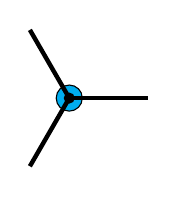
\begin{tikzpicture}
        \node at (0,0) [circle,draw,fill=cyan] (a) {};
        \fill (0,0) circle [radius=2pt,fill=black];
        \draw [ultra thick] (0,0) -- +(0:1cm);
        \draw [ultra thick] (0,0) -- +(120:1cm);
        \draw [ultra thick] (0,0) -- +(240:1cm);
    \end{tikzpicture}
    \caption{Three surface sides}
  \end{subfigure}
  \begin{subfigure}[c]{0.3\textwidth}
    \centering
    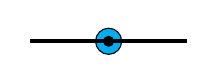
\begin{tikzpicture}
        \node at (0,0) [circle,draw,fill=cyan] (a) {};
        \fill (0,0) circle [radius=2pt,fill=black];
        \draw [ultra thick] (0,0) -- +(0:1cm);
        \draw [ultra thick] (0,0) -- +(180:1cm);
    \end{tikzpicture}
    \caption{Two surface sides}
  \end{subfigure}
  \caption{Examples of surface cardinality}
\end{figure}

For one of the sets surface cardinality of~$a$ is $3$ and for
another it is~$2$.

Now define \emph{shift special points}.

Let $I$ be an interval on~$\mathbb{R}$ (containing zero?)

A point~$a$ is \emph{shift special} if there exists a transformation
(that is a continuous function $f:I\times\mu\to\mu$ such that:
\begin{enumerate}
  \item $f(0)$ is identity. \fxwarning{Is this condition needed?}
  \item for every sufficiently small~$\epsilon>0$ we have $f(\epsilon,a)\in T$;
  \item there is $\epsilon>0$ such that for every $0<\epsilon'<\epsilon$ we have
    $f(\epsilon')$ being not continuous at~$a$ regarding complete funcoid
    defined by the function $x\mapsto\rsupfun{\mu}\{x\}\setminus T$.
\end{enumerate}

We may consider to additonally require that every~$f(\epsilon)$ is isomorphism
of funcoids.

\begin{example}
$T$~is disk $\setcond{(x,y,0)}{x^2+y^2\leq 1}$. $f$~is the contraction
$(\epsilon,v)\mapsto\frac{1}{1+\epsilon}v$. $a=(1,0,0)$.

In the usual topology~$f$ is continuous. In
$x\mapsto\rsupfun{\mu}\{x\}\setminus T$ we have the function
$\epsilon\mapsto f(\epsilon)$ not continuous at zero.
So~$a$ is a shift special point.
\end{example}

\begin{proof}
$f (0) (v) = v$. Thus $\langle f (0) \rangle (\rsupfun{\mu} \{ a
\} \setminus T) = \rsupfun{\mu} \{ a \} \setminus T$ intersects
the plane $Z = 0$. But $f (0, a)$

??
\end{proof}

\begin{question}
Can we exclude real numbers from the play?
\end{question}

\begin{question}
How cardinality special points, isomorphism special points and shift
special points are related with each others?
\end{question}

\begin{question}
How the number of surface sides is related with usual surface sides for
manifolds?
\url{https://en.wikipedia.org/wiki/Orientability#Orientability_of_manifolds}
\end{question}

\begin{rem}
Manifolds have no special points. (Prove!)
\end{rem}

Prove that $2$-manifold image which special points removed has the same number
of sides as the defined above.

Another way to define special points: A special point is a point
such that $T\sqcap\supfun{\mu}\{a\}$ is not isomorphic to
$T\sqcap\supfun{\mu}\{x\}$ for nearby points~$x$. Consider replacement
of isomorphism with injection, surjection, etc. here and above.

How many sides has in $\mathbb{R}^3$ a plane without one point?

Easy way to spot special points: They are boundary points in the
topology (or funcoid) induced on~$T$. Alternatively we can consider
points whose neighborhood in~$T$ is different (as non-isomorphic or
maybe non-injective or non-surjective or like this) than of nearby
points. Thus another way to remove special points: use interior funcoid.

\url{https://math.stackexchange.com/q/2836833/4876}


% \printindex{}

\bibliographystyle{plain}
\bibliography{refs}

\end{document}
